%% bare_conf.tex
%% V1.3
%% 2007/01/11
%% by Michael Shell
%% See:
%% http://www.michaelshell.org/
%% for current contact information.
%%
%% This is a skeleton file demonstrating the use of IEEEtran.cls
%% (requires IEEEtran.cls version 1.7 or later) with an IEEE conference paper.
%%
%% Support sites:
%% http://www.michaelshell.org/tex/ieeetran/
%% http://www.ctan.org/tex-archive/macros/latex/contrib/IEEEtran/
%% and
%% http://www.ieee.org/

%%*************************************************************************
%% Legal Notice:
%% This code is offered as-is without any warranty either expressed or
%% implied; without even the implied warranty of MERCHANTABILITY or
%% FITNESS FOR A PARTICULAR PURPOSE! 
%% User assumes all risk.
%% In no event shall IEEE or any contributor to this code be liable for
%% any damages or losses, including, but not limited to, incidental,
%% consequential, or any other damages, resulting from the use or misuse
%% of any information contained here.
%%
%% All comments are the opinions of their respective authors and are not
%% necessarily endorsed by the IEEE.
%%
%% This work is distributed under the LaTeX Project Public License (LPPL)
%% ( http://www.latex-project.org/ ) version 1.3, and may be freely used,
%% distributed and modified. A copy of the LPPL, version 1.3, is included
%% in the base LaTeX documentation of all distributions of LaTeX released
%% 2003/12/01 or later.
%% Retain all contribution notices and credits.
%% ** Modified files should be clearly indicated as such, including  **
%% ** renaming them and changing author support contact information. **
%%
%% File list of work: IEEEtran.cls, IEEEtran_HOWTO.pdf, bare_adv.tex,
%%                    bare_conf.tex, bare_jrnl.tex, bare_jrnl_compsoc.tex
%%*************************************************************************

% *** Authors should verify (and, if needed, correct) their LaTeX system  ***
% *** with the testflow diagnostic prior to trusting their LaTeX platform ***
% *** with production work. IEEE's font choices can trigger bugs that do  ***
% *** not appear when using other class files.                            ***
% The testflow support page is at:
% http://www.michaelshell.org/tex/testflow/



% Note that the a4paper option is mainly intended so that authors in
% countries using A4 can easily print to A4 and see how their papers will
% look in print - the typesetting of the document will not typically be
% affected with changes in paper size (but the bottom and side margins will).
% Use the testflow package mentioned above to verify correct handling of
% both paper sizes by the user's LaTeX system.
%
% Also note that the "draftcls" or "draftclsnofoot", not "draft", option
% should be used if it is desired that the figures are to be displayed in
% draft mode.
%
% \documentclass[draftcls]{IEEEtran}
\documentclass[journal]{IEEEtran}
% Add the compsoc option for Computer Society conferences.
%
% If IEEEtran.cls has not been installed into the LaTeX system files,
% manually specify the path to it like:
% \documentclass[conference]{../sty/IEEEtran}





% Some very useful LaTeX packages include:
% (uncomment the ones you want to load)


% *** MISC UTILITY PACKAGES ***
%
%\usepackage{ifpdf}
% Heiko Oberdiek's ifpdf.sty is very useful if you need conditional
% compilation based on whether the output is pdf or dvi.
% usage:
% \ifpdf
%   % pdf code
% \else
%   % dvi code
% \fi
% The latest version of ifpdf.sty can be obtained from:
% http://www.ctan.org/tex-archive/macros/latex/contrib/oberdiek/
% Also, note that IEEEtran.cls V1.7 and later provides a builtin
% \ifCLASSINFOpdf conditional that works the same way.
% When switching from latex to pdflatex and vice-versa, the compiler may
% have to be run twice to clear warning/error messages.






% *** CITATION PACKAGES ***
%
%\usepackage{cite}
% cite.sty was written by Donald Arseneau
% V1.6 and later of IEEEtran pre-defines the format of the cite.sty package
% \cite{} output to follow that of IEEE. Loading the cite package will
% result in citation numbers being automatically sorted and properly
% "compressed/ranged". e.g., [1], [9], [2], [7], [5], [6] without using
% cite.sty will become [1], [2], [5]--[7], [9] using cite.sty. cite.sty's
% \cite will automatically add leading space, if needed. Use cite.sty's
% noadjust option (cite.sty V3.8 and later) if you want to turn this off.
% cite.sty is already installed on most LaTeX systems. Be sure and use
% version 4.0 (2003-05-27) and later if using hyperref.sty. cite.sty does
% not currently provide for hyperlinked citations.
% The latest version can be obtained at:
% http://www.ctan.org/tex-archive/macros/latex/contrib/cite/
% The documentation is contained in the cite.sty file itself.






% *** GRAPHICS RELATED PACKAGES ***
%
\ifCLASSINFOpdf
  % \usepackage[pdftex]{graphicx}
  % declare the path(s) where your graphic files are
  % \graphicspath{{../pdf/}{../jpeg/}}
  % and their extensions so you won't have to specify these with
  % every instance of \includegraphics
  % \DeclareGraphicsExtensions{.pdf,.jpeg,.png}
\else
  % or other class option (dvipsone, dvipdf, if not using dvips). graphicx
  % will default to the driver specified in the system graphics.cfg if no
  % driver is specified.
  % \usepackage[dvips]{graphicx}
  % declare the path(s) where your graphic files are
  % \graphicspath{{../eps/}}
  % and their extensions so you won't have to specify these with
  % every instance of \includegraphics
  % \DeclareGraphicsExtensions{.eps}
\fi
% graphicx was written by David Carlisle and Sebastian Rahtz. It is
% required if you want graphics, photos, etc. graphicx.sty is already
% installed on most LaTeX systems. The latest version and documentation can
% be obtained at: 
% http://www.ctan.org/tex-archive/macros/latex/required/graphics/
% Another good source of documentation is "Using Imported Graphics in
% LaTeX2e" by Keith Reckdahl which can be found as epslatex.ps or
% epslatex.pdf at: http://www.ctan.org/tex-archive/info/
%
% latex, and pdflatex in dvi mode, support graphics in encapsulated
% postscript (.eps) format. pdflatex in pdf mode supports graphics
% in .pdf, .jpeg, .png and .mps (metapost) formats. Users should ensure
% that all non-photo figures use a vector format (.eps, .pdf, .mps) and
% not a bitmapped formats (.jpeg, .png). IEEE frowns on bitmapped formats
% which can result in "jaggedy"/blurry rendering of lines and letters as
% well as large increases in file sizes.
%
% You can find documentation about the pdfTeX application at:
% http://www.tug.org/applications/pdftex




\usepackage{bbm}
\usepackage{verbatim}
\usepackage{graphicx}
\usepackage{cite}
\usepackage{url}
\usepackage[cmex10]{amsmath}
\usepackage{amssymb}
\usepackage{amsmath}
% \usepackage{algorithm,algorithmic}
\usepackage{algorithm, algorithmicx, algpseudocode}
%\usepackage{algpseudocode}
% \usepackage{cases}
\usepackage[caption=false,font=footnotesize]{subfig}
\usepackage{color}
\usepackage{cite}
\usepackage{epstopdf}
\usepackage{calc}
\usepackage{array}
% \usepackage{accents}
\usepackage{multirow}
% \usepackage{subfigure}


\newtheorem{proposition}{Proposition}

\DeclareMathOperator*{\argmax}{arg\,max} % Jan Hlavacek
\DeclareMathOperator{\cov}{cov}
\DeclareMathOperator{\diag}{\mathrm{diag}}

\newcommand{\vw}[1]{\mathbf{w}_{#1}}
\newcommand{\vy}[1]{\mathbf{y}_{#1}}
\newcommand{\vs}[1]{\mathbf{s}_{#1}}
\newcommand{\vn}[1]{\mathbf{n}_{#1}}
\newcommand{\vH}[1]{\mathbf{H}_{#1}}
\newcommand{\vr}[0]{\mathbf{r}}
\newcommand{\vR}[0]{\mathbf{R}}
\newcommand{\vW}[1]{\mathbf{W}_{#1}}

\newcommand{\sub}[0]{\text{s}}

\newcommand{\va}[1]{\mathbf{a}_{#1}}
\newcommand{\vA}[1]{\mathbf{A}_{#1}}

\newcommand{\tx}[0]{\text{T}}
\newcommand{\rx}[0]{\text{R}}


\newcommand{\hermitian}[0]{\text{H}}
\newcommand{\transpose}[0]{\text{T}}
\newcommand{\fro}[0]{\text{F}}
\newcommand{\ie}[0]{\textit{i.e.}}
\newcommand{\veta}[0]{\boldsymbol{\eta}}
\newcommand{\CFO}[0]{\epsilon_{\text{F}}}
\newcommand{\STO}[0]{\epsilon_{\text{T}}}
\newcommand{\Ts}[0]{T_{\text{s}}}
\newcommand{\Tb}[0]{T_{\text{B}}}
\newcommand{\Nb}[0]{N_{\text{B}}}
\newcommand{\Nc}[0]{N_{\text{c}}}
\newcommand{\Ncp}[0]{N_{\text{cp}}}
\newcommand{\sigman}[0]{\sigma_{\text{n}}}
\newcommand{\TSS}[0]{T_{\text{F}}}
\newcommand{\var}[0]{\mathrm{var}}
\newcommand{\Q}[0]{\mathrm{Q}}
\newcommand{\Qinv}[0]{\mathrm{Q}^{-1}}
\newcommand{\SNR}[0]{\mathrm{SNR}}
\newcommand{\Gr}[0]{G_{\text{R}}}
\newcommand{\Gt}[0]{G_{\text{T}}}
\newcommand{\Gd}[0]{G_{\text{D}}}
\newcommand{\prob}[0]{\mathrm{Pr}}
\newcommand{\NUE}[0]{N_{\text{U}}}



% correct bad hyphenation here
\hyphenation{op-tical net-works semi-conduc-tor}


\begin{document}
% \onecolumn
%
% paper title
% can use linebreaks \\ within to get better formatting as desired
\title{Compressive Initial Access and Beamforming Training in Millimeter-Wave Networks}


% author names and affiliations
% use a multiple column layout for up to three different
% affiliations
\author{Han~Yan,~\IEEEmembership{Student~Member,~IEEE},~and~Danijela~Cabric,~\IEEEmembership{Senior~Member,~IEEE}%
% \thanks{Manuscript received xxx; revised xxx. This work was supported by the xxx.}%
\thanks{Han Yan and Danijela Cabric are with the Electrical and Computer Engineering Department, University of California, Los Angeles, Los Angeles, CA 90095 (e-mail: yhaddint@ucla.edu; danijela@ee.ucla.edu).}
\thanks{Part of work was presented in IEEE GlobalSIP 2016 \cite{hyan_mmWave_CFO}}
\thanks{This work was supported by part under NSF grant 1718742.}
}

% conference papers do not typically use \thanks and this command
% is locked out in conference mode. If really needed, such as for
% the acknowledgment of grants, issue a \IEEEoverridecommandlockouts
% after \documentclass



% use for special paper notices
% \IEEEspecialpapernotice{(Invited Paper)
% \vspace{-8mm}
% }



% make the title area
\maketitle

%%%%%%%%%%%%%%%%%%%%%%%%%%%%%%%%%%%%%%%%%%%%%%%%%%%%%%%%%%%%%%%%%%%%%%%%%%%%%%%
%%%%%%%%%%%%%%%%%%%%%%%%%%%%%%%%%%%%%%%%%%%%%%%%%%%%%%%%%%%%%%%%%%%%%%%%%%%%%%%

\begin{abstract}
Initial access (IA) is a fundamental physical layer procedure in cellular systems where user equipment (UE) detect nearby base station (BS) as well as acquire synchronization. Due to the necessity of using antenna array in millimeter wave (mmW) IA, the spatial information of channel can also be inferred. The state-of-the-art directional IA (DIA) uses sector sounding beams which fails to provide decent angular resolution and therefore beam training with dedicated radio resources are required. To avoid the extra access latency and overhead, this work proposes to use a quasi-omni pseudorandom sounding beam in IA. In particular, we develop a novel algorithm where the UE can jointly achieve initial access and precise initial beam training without extra radio resources. We study the miss detection rate of the proposed algorithm under synchronization error, and further derive  Cram\'er-Rao lower bound of direction estimation under frequency offset. Using QuaDRiGa simulator with mmMAGIC model, the numerical results show that the proposed approach is advantageous to DIA paired with hierarchy beam training. It offers up to two order of magnitude access latency saving when the same discovery, post training SNR, and overhead performance are targeted and such conclusion holds true in various propagation environment and 3D locations with a mmW pico-cell with up to 140 m radius. 
\end{abstract}


% Index: a
% \end{keywords}

%%%%%%%%%%%%%%%%%%%%%%%%%%%%%%%%%%%%%%%%%%%%%%%%%%%%%%%%%%%%%%%%%%%%%%%%%%%%%%%
%%%%%%%%%%%%%%%%%%%%%%%%%%%%%%%%%%%%%%%%%%%%%%%%%%%%%%%%%%%%%%%%%%%%%%%%%%%%%%%
\section{Introduction}
\label{sec:Introduction}

% common ground: millimeter wave & beam training
% \subsection{Motivation}
Millimeter-wave (mmW) communication is a promising technology for the future cellular network including 5G New Radio (5G-NR) \cite{Andrew:what5Gbe}. The mmW network supports ultra-fast data rate due to the abundant bandwidth. As shown in both theory and prototypes, mmW system requires beamforming (BF) with large antenna arrays at both base station (BS) and user equipment (UE) to combat severe propagation loss \cite{Rappaport:mmWavewillwork}. 
% The nature of large antenna in higher frequency band make people rethink the tranceivers architecture and new array architecture including hybrid analog and digital beamforming using digital processor together with analog phased shifter [ref]. 
Significant change in propagation characteristic and hardware architecture in mmW band require different signal processing techniques \cite{7400949} and physical layer procedure \cite{3GPP_PHY_study}.

Initial access (IA) is one of the fundamental physical layer procedure that is expected to be changed in mmW networks as compared to sub-6GHz band networks. IA allows UE to discover and synchronize with nearby BS before further communication. 
% Conventionally, the base station periodically broadcast a special synchronization beacon. When not currently associated with BS, a UE would actively search for such signal and reaches synchronization with BS. 
In mmW system, conventional omni-directionally broadcast IA with single antenna may not be reliable enough. It is the consensus that IA also needs to use transmitter and receiver antenna array \cite{7161389,Giordani_beam_turotial_arxiv_1804}. A key challenge is the sounding beam design during IA for reliable discovery.
% This feature makes initial BF training a crucial and challenging task: mmW system requires aligned transmission and reception beams to meets link budget, but BF training itself is carried out with low SNR and poor synchronization. Besides, the time and hardware cost becomes prohibitively high if BF training methods in current microwave system are directly applied to the mmW system with larger antenna arrays. 
Meanwhile, beam training is an equally important procedure in order to reap the BF gain from large arrays. A key challenge in beam training is to avoid the excessive access latency and signaling overhead during channel probing. 
% In the conventional sub-6GHz band, beamforming training is completely independent with IA. In fact, it uses dedicated time slot where dedicated pilot sequence is used to estimate channel from each antenna pair from transmitter and receiver and orthogonal time slots is used for additional antennas \cite{6798744}.

% It is expected that in mmW mobile networks, the functionality between initial access and beamforming training are more vague. 

 % is expected to be aligned with initial access procedure [directional discovery from NYU].

% this procedure is after initial access and it uses dedicated time slot where dedicated pilot sequence is used to estimate channel from each antenna pair from transmitter and receiver and orthogonal time slots is used for additional antennas [massive MIMO channel estimation paper]. However, the requires overhead scales linearly with antenna size and may not efficient enough for massive array regime [sub-6GHz massive MIMO channel estimation paper]. More importantly, it does not directly applicable to mmW array where fully digital architecture is not available. Due to the sparse scattering nature, mmW signal propagates between transmitter and receiver through a few directions [ref]. Such sparse channel implies that once dominant propagation directions are estimated, channel capacity can be approached. 

% Therefore, novel signal processing algorithms are needed in mmW initial BF training, especially algorithms exploiting sparsity of the mmW channel \cite{7400949}.

% Channel estimation is another important topic. Conventionally in sub-6GHz band, this procedure is after initial access and it uses dedicated time slot where dedicated pilot sequence is used to estimate channel from each antenna pair from transmitter and receiver and orthogonal time slots is used for additional antennas [massive MIMO channel estimation paper]. However, the requires overhead scales linearly with antenna size and may not efficient enough for massive array regime [sub-6GHz massive MIMO channel estimation paper]. More importantly, it does not directly applicable to mmW array where fully digital architecture is not available. Due to the sparse scattering nature, mmW signal propagates between transmitter and receiver through a few directions [ref]. Such sparse channel implies that once dominant propagation directions are estimated, channel capacity can be approached. 

 

% related works
\subsection{Related works}

A number of works investigate sounding beam and processing algorithm design in mmW IA and beam training.

Using directional beam in IA and beam training is investigated in \cite{7161389,Caire_DIA_arxiv_1709,UTA_stocha_geo_IA_TCOM_18,KTH_stoch_geo_IA_arxiv_1802,Meng_OIA_TCOM_1803,Zorzi_IA_MCOM_1611,UTA_IA_TWC_1705,Giordani_beam_turotial_arxiv_1804,6847111,7914759}. Directional IA (DIA) is first studied in \cite{7161389} and a General Likelihood Ratio Test (GLRT) is proposed to the solve the cell discovery problem with unknown channel and synchronization parameters. The authors also conclude that the directionally beamformed IA signal improves discovery range as compared to omni-directional IA. The DIA is further investigated in \cite{Caire_DIA_arxiv_1709} where overhead and access latency are analyzed. Work \cite{UTA_stocha_geo_IA_TCOM_18} and \cite{KTH_stoch_geo_IA_arxiv_1802} study DIA in large networks, and access latency is studied using stochastic geometry. Impact of beam-width of sounding beams in DIA is researched in \cite{UTA_IA_TWC_1705}. The comparison between omni-directional and DIA is also discussed in \cite{Meng_OIA_TCOM_1803}. IA using non-in-band information, e.g., location, sub-6GHz measurement, are discussed in \cite{Zorzi_IA_MCOM_1611,Giordani_beam_turotial_arxiv_1804}. The above works mostly focus on the overhead and latency for the cell discovery while beam training is not discussed or with coarse resolution \cite{Caire_DIA_arxiv_1709}. Part of the reasons are that DIA commonly pair with directional beam training \cite{6847111,7914759} where hierarchical sounding beams are used in multiple stages for precise training. However, the user-specific hierarchy sounding beam adaptation introduces latency when the BS is connected with large number of UEs.

The alternative beam training is via the parametric channel estimation \cite{7390019,7178503,8306126,7472310,8356247,8488662,8323164,7914742}. Exploiting the mmW sparse scattering nature, compressive sensing (CS) can effectively estimate channel parameters using channel observations through sounding beams. Works \cite{7390019,7178503} propose a CS-based narrowband BF training use pseudo-random noise (PN) sounding beams in the downlink, and \cite{8306126} extends into wideband channel. Other notable works include channel covariance estimation \cite{7472310,8356247,8488662} which requires periodic channel observations, and UE centric uplink training \cite{8323164,7914742}. The above works focus on channel estimation in the dedicated training slots and assume perfect cell discovery and synchronization. The 5G-NR frame structure is rarely considered and thus the feasibility of joint initial access and CS-based beam training are not investigated. 


% A CS-based BF training hardware prototype is reported in \cite{7146023} and it demonstrates the training efficacy when synchronization is resolved by cabled reference clock. 
To address the issues of frequency synchronization in narrowband mmW beam training, novel algorithms are proposed in \cite{hyan_mmWave_CFO,Myers_CFO_SPAWC_1707,8309152,Myers_CFO_arxiv_1803}. Meanwhile, hardware prototypes that use received signal strength (RSS) in CS-based beam training are reported and the signal processing tools include RSS matching pursuit \cite{Rasekh_noncoherentCS_ACM_2017}, Hashing table \cite{Hassanieh:2018:FMW:3230543.3230581}, and sparse phase retrieval \cite{UCSB_noncoherentCS_arxiv_1801}. However, such phase free measurement is a testbed dependent constraint and does not necessarily apply to all mmW systems. Moreover, the theoretical accuracy limits and practical signal processing algorithm tailored for initial discovery, synchronization, and BF training in mmW frequency selective channel are not yet fully addressed. 


% A CS-based BF training hardware prototype is reported in \cite{7146023}. However, the cabled reference clock setting in \cite{7146023} raises concern of phase measurement accuracy during beam training, which leads to the recent studies of the joint carrier synchronization and narrowband BF training \cite{Myers_CFO_SPAWC_1707,8309152,Myers_CFO_arxiv_1803} as well as the early version of this work \cite{hyan_mmWave_CFO}. Meanwhile, 


% Works \cite{Rasekh_noncoherentCS_ACM_2017,UCSB_noncoherentCS_arxiv_1801} use magnitude information from compressive channel sounding and it avoids phase synchronization errors. 
% Compensation phase error in this procedure is investigated in the early presentation of this work \cite{hyan_mmWave_CFO} as well as \cite{Myers_CFO_SPAWC_1707,8309152} using hybrid array architecture and \cite{Myers_CFO_arxiv_1803} using 1-bit quantization array architecture. However, an comprehensive theoretical analysis was not available in the literature.

% Works \cite{7390019,7178503} proposed to use random precoding and combining matrices for BF training. This CS-based method allows multiple UEs to estimate channel and align their beams simultaneously. Using the adaptive compressive sensing, the training duration can be further shortened since BS and UE adapt their BF training vectors based on results from previous training slots \cite{6847111}. But those works all assume perfect synchronization between BS and UE. A prototype of CS-based BF training developed in \cite{7146023} avoids synchronization issue by connecting transmitter and receiver with same external clock.

%%%%%%%%%%%%%%%%%%%%%%%%%%%%%%%%%%%%%%%%%%%%%%%%%%%%%%%%%%%%%%%%%%%%%%%%%%%%%%%
%%%%%%%%%%%%%%%%%%%%%%%%%%%%%%%%%%%%%%%%%%%%%%%%%%%%%%%%%%%%%%%%%%%%%%%%%%%%%%%
% contributions
\subsection{Contributions}
In this work, we propose to use PN sounding beams and novel signal processing algorithm to jointly achieves initial cell discovery, synchronization, and accurate beam training. The contributions are answers to the following questions.
% \begin{itemize}

\textit{How to use PN sounding beam for IA?} We propose an energy detection algorithm for initial discovery and it is tailored for PN sounding beams. We derive the optimal detection threshold, analyze the miss detection probability and the impact of synchronization error, i.e., carrier frequency offset (CFO) and timing offset (TO).

\textit{How to reuse received IA signal for beam training?} We propose algorithm that re-processes the received IA signal for initial beam training and synchronization once cell detection occurs. We derive the Cram\'er-Rao lower bound (CRLB) of training performance in line-of-sight (LOS). A CS-based algorithm is proposed that is effective in non-LOS (NLOS) environments and reaches CRLB in LOS.
% We reveal that the proposed algorithm facilitates near perfect BF training performance so long as UE can discover the BS.

\textit{What are the benefits of compressive IA?} We compare the proposed approach with DIA paired by hierarchy beam training. Performance indicators of both approaches are numerically compared, including discovery rate, post beam training SNR, overhead and access latency. The simulation with 5G-NR frame structure and measurement-endorsed 3D mmW channel shows that the proposed approach is advantageous to DIA for UE in various locations of a small cell.


%%%%%%%%%%%%%%%%%%%%%%%%%%%%%%%%%%%%%%%%%%%%%%%%%%%%%%%%%%%%%%%%%%%%%%%%%%%%%%%

%paper organization

%%%%%%%%%%%%%%%%%%%%%%%%%%%%%%%%%%%%%%%%%%%%%%%%%%%%%%%%%%%%%%%%%%%%%%%%%%%%%%%
\subsection{Organizations and notations}
The rest of the paper is organized as follows. We start with a brief introduction of 5G-NR frame structure, IA and beam training in Section~\ref{sec:preliminary}. In Section~\ref{sec:system_model}, we present the system model and problem statement. Section~\ref{sec:cell_discovery} includes the proposed algorithm for cell discovery and timing acquisition followed by associated performance analysis. In Section~\ref{sec:CS_based_training} we present the algorithm and analysis for initial beam training under CFO. The access latency, overhead, and complexity analysis is included in Section~\ref{sec:comparison_analysis}. The numerical results are presented in Section~\ref{sec:simulation results}. Open research issues are summarized in Section~\ref{sec:discussion}. Finally, Section~\ref{sec:Conclusion} concludes the paper.

%%%%%%%%%%%%%%%%%%%%%%%%%%%%%%%%%%%%%%%%%%%%%%%%%%%%%%%%%%%%%%%%%%%%%%%%%%%%%%%
%%%%%%%%%%%%%%%%%%%%%%%%%%%%%%%%%%%%%%%%%%%%%%%%%%%%%%%%%%%%%%%%%%%%%%%%%%%%%%%

\textit{Notations:} Scalars, vectors, and matrices are denoted by non-bold, bold lower-case, and bold upper-case letters, respectively, e.g. $h$, $\mathbf{h}$ and $\mathbf{H}$. The $(i,j)$-th element of $\mathbf{H}$ is denoted by $[\mathbf{H}]_{i,j}$. Conjugate, transpose, Hermitian transpose, and Moore-Penrose pseudoinverse are denoted by $(.)^{*}$, $(.)^{\transpose}$, $(.)^{\hermitian}$, and $(.)^{\dagger}$ respectively. The inner product is $\langle \mathbf{a},\mathbf{b}\rangle  \triangleq  \mathbf{a}^{\hermitian}\mathbf{b}$. The $l_2$-norm of $\mathbf{h}$ is denoted by $||\mathbf{h}||$. $\diag(\mathbf{A})$ aligns diagonal elements of $\mathbf{A}$ into a vector and $\diag(\mathbf{a})$ aligns vector $\mathbf{a}$ into a diagonal matrix. Kronecker and Hadamard product are denoted as $\otimes$ and $\circ$, respectively. $\Re(x)$ and $\Im(x)$ are the real and imaginary parts of a complex element $x$, respectively.

% organizations
% This paper is organized as follows. In Sect.~II, the system model of mmWave system is described. Sect.~III introduces compressive sensing based alignment training and its delay is analyzed. In Sect.~III, double-stage training method is presented. In Sect.~IV, we numerical evaluate and compare the performance of single-stage and two. We conclude the results in Sect.~VI.

%%%%%%%%%%%%%%%%%%%%%%%%%%%%%%%%%%%%%%%%%%%%%%%%%%%%%%%%%%%%%
\section{Preliminary: initial access and beam training}
\label{sec:preliminary}
In this section, we introduce the mmW physical layer frame structure and procedure in 5G-NR cellular network. We briefly review the frame structure, synchronization sequences, and directional IA scheme as well as beam training. Reader are referred to work \cite{Giordani_beam_turotial_arxiv_1804} for a more detailed survey.
\begin{figure}
\begin{center}
\includegraphics[width=0.48\textwidth]{figures/5GNR_farme_structure}
\end{center}
\vspace{-4mm}
\caption{The 5G-NR mmW frame structure with emphasis in beam management function and the illustration for directional initial access.}
\vspace{-4mm}
\label{fig:frame_structure}
\end{figure}

%%%%%%%%%%%%%%%%%%%%%%%%%%%%%%%%%%%%%%%%%%%%%%%%%%%%%%%%%%%%%
\textit{Frame Structure:} Fig.~\ref{fig:frame_structure} shows the frame structure of 5G-NR mmW, and we focus on two functional block, synchronization sequence (SS) burst and channel state information reference signal (CSI-RS). 5G-NR uses orthogonal frequency division multiplexing (OFDM), and the subcarrier spacing is either $120 \text{ or } 240$ KHz for mmW band. The SS signal is transmitted by a BS with period $\TSS$, typically 20 ms. The SS consists of up to $M=64$ burst blocks. In each one of the burst block with duration $T_{\text{B}}$, a specific sounding beam pair is used by BS and UE. The CSI-RS block with duration $T_{\text{r}}$ is dedicated resource for specific UE(s) for beam training and tracking and CSI-RS has periodicity $T_{\text{R}}$, whose value is implementation dependent.
% A fixed number of CSI-RS are available within $\TSS$ and we denote it as $K_{\text{R}}$. 
% Note that when large number of UEs are connected with BS, CSI-RS resources need to be scheduled among them.

\textit{Synchronization Sequence:}
Refer to Fig.~\ref{fig:frame_structure}, each SS burst has 4 OFDM symbols, i.e., primary synchronization signal (PSS), physical broadcast channel (PBCH), and secondary synchronization signal (SSS). PSS is used in cell detection and synchronization and they are assigned to the middle $P=128$ subcarriers of the first OFDM symbols. \color{black} The PSS is Zadoff-Chu (ZC) sequences in 4G-LTE due to their perfect cyclic-autocorrelation property \cite{4373412}, and becomes Maximum Length Sequences (M-sequences) in 5G-NR \cite{3GPP_modulation}. There are 3 and 336 unique sequences of PSS and SSS, respectively, and these 1008 combination defines the cell identifiers (ID) of BS. PBCH carries control information, e.g., channel bandwidth. \color{black}

%%%%%%%%%%%%%%%%%%%%%%%%%%%%%%%%%%%%%%%%%%%%%%%%%%%%%%%%%%%%%
\textit{Beamformed Initial Access:}
The BS periodically transmits IA blocks and such signals are processed by UEs which desire to establish the initial access, reconnects after beam misalignment, and search for additional BS for potential handover. The sounding beams in SS bursts intend to facilitate multi-antenna processing in BS and UE when no-priori channel information is available. In the DIA scheme, BS and UE use $M_{\tx}$ and $M_{\rx}$ transmitter and receiver beams to cover angular space in both ends and one T/Rx beam is used at a time in the $M=M_{\tx}M_{\rx}$ SS bursts. Example of such beam sweeping is shown in Fig.~\ref{fig:frame_structure}.

 % of 2D DIA is to cover angle range $\theta^{(d)}_{m_{\tx}}$ in BS and $\phi^{(d)}_{m_{\rx}}$ in UE during the $[(m_{\rx}-1)M_{\tx} + m_{\tx}]$-th SS burst. Sector beams cover the entire angular plane as
% \begin{align}
% \begin{split}
% \theta^{\text{(d)}}_{m_{\tx}} = &[-\frac{\pi}{2} + \frac{\pi(m_{\tx}-1)}{M_{\tx}+1}, -\frac{\pi}{2} + \frac{\pi m_{\tx}}{M_{\tx}+1}],\quad m_{\tx}\in [1,M_{\tx}],\\
% \phi^{\text{(d)}}_{m_{\rx}} = &-\frac{\pi}{2} + \frac{\pi(m_{\rx}-1)}{M_{\rx}-1},\quad m_{\rx}\in [1,M_{\rx}].
% \end{split}
% \label{eq:dir_pointing_angle}
% \end{align}

%%%%%%%%%%%%%%%%%%%%%%%%%%%%%%%%%%%%%%%%%%%%%%%%%%%%%%%%%%%%%

\textit{Beam Training:} 
The sounding beams in DIA typically have large beam-width and flat response inside angular sectors \cite{7845674}. Such design covers the angular space of BS and UE within $M$ bursts, but allows coarse propagation directions estimation \cite{Caire_DIA_arxiv_1709}. Beam training facilitates higher angular resolution where BS and UE steer narrow sounding beams within the sectors of interest. This procedure requires CSI-RS as radio resource.



% \textit{Omnidirectional IA in 4G-LTE:}
% This cell search procedure is performed both by UEs in idle mode, either seeking to establish an initial access to a base station or to find an eNB cell to “camp on” for paging, or UEs that are already connected to a base station, aka, evolved Node B (eNB), and need to look for other eNBs for potential handover targets. After detecting an eNB through the cell search, UEs in idle mode can initiate a random access procedure to the cell to establish a connection to the eNB, should a transition to active mode be necessary. UEs that are already connected to a serving eNB can report the signal strengths of the detected cell IDs to the network, which can then command the UE to perform a handover to that cell.

%%%%%%%%%%%%%%%%%%%%%%%%%%%%%%%%%%%%%%%%%%%%%%%%%%%%%%%%%%%%%%
%
% 							Section 2: System Model and Algorithm
%
%%%%%%%%%%%%%%%%%%%%%%%%%%%%%%%%%%%%%%%%%%%%%%%%%%%%%%%%%%%%%
\section{System Model}
\label{sec:system_model}
% In this section, we first introduce the preliminary of initial access in 5G-NR including frame structure and IA protocol. Then we describe the system model for the proposed compressive IA scheme, which has two major stage: initial discovery and initial beamforming training.

This section introduces the system model that adopts the above 5G-NR frame structure and problem formulation of the compressive initial access and beam training. \color{black}All important notations are summarized in Table~\ref{tab:notation}. \color{black}
\begin{table}
\caption{Nomenclature}
\centering
\begin{tabular}{|c|c|}
\hline 
Symbol &Explanations\tabularnewline
\hline 
\hline 
% Carrier Frequency & $f_c = 28$ GHz\tabularnewline
% \hline 
$p$, $P$ &  Index and total number of subcarriers\tabularnewline
$m$, $M$ &  Index and total number of SS bursts\tabularnewline
$l, L$  & Index and total number of multipaths \tabularnewline
\hline 
$N_{\tx}$, $N_{\rx}$  & Number of antenna in BS and UE\tabularnewline
$\Ts$ &  Sample duration of IA signal\tabularnewline 
$\Tb,\Nb$ &  Duration and sample number in each SS burst\tabularnewline
$\TSS$ &  Period of SS bursts\tabularnewline
$T_{\text{R}}$,$T_{\text{r}}$ &  Period and duration of CSI-RS\tabularnewline
$\Nc$, $\Ncp$ &  Max. excess delay taps and length of CP\tabularnewline
$N_{\text{train}},N_{\text{U}}$ &  Required CSI-RS and UE number\tabularnewline
\hline 
$\Delta f$, $\epsilon_{\text{F}}$ &  CFO in [Hz] and normalized in [rad/samp.] \tabularnewline
% $\epsilon_{\text{F}}$ &  Initial CFO in UE (normalized with $\Ts$)\tabularnewline
$\epsilon_{\text{T}}$ &  Initial TO in UE (number of sample) \tabularnewline
\hline 
$\mathbf{H}[d]$ & MIMO channel at $d$-th delay sample\tabularnewline
$\mathbf{a}_{\tx}\left(\theta\right)$, $\mathbf{a}_{\rx}\left(\phi\right)$   & Spatial responses of BS and UE\tabularnewline
% $\mathbf{a}_{\rx}\left(\phi\right)$  & Spatial responses of UE ULA\tabularnewline
$\phi_l,\theta_l$, $g_l$, $\tau_l$  &Gain/AoA/AoD/delay of $l$-th multipath  \tabularnewline
% $g_l$  & Complex channel gain of $l$-th multipath  \tabularnewline
$\alpha_l, \beta_l$  & Real and imaginary parts of $g_l$  \tabularnewline
% $\tau_l$  & Exces. Delay of $l$-th multipath  \tabularnewline
\hline 
$\mathbf{s}, \tilde{\mathbf{s}}$, $\tilde{s}[n]$ & F/T domain PSS vector and sequence\tabularnewline
% $\tilde{s}[n]$ &  T-domain. PSS sequence\tabularnewline
$\mathbf{v}_m, \mathbf{w}_m$ & RF precoder/combiner of the $m$-th burst\tabularnewline
$z[n]$, $\mathbf{z}_m$, $\sigman^2$ & AWGN sequence, vector, and power\tabularnewline
% $\mathbf{z}_m$  & AWGN vector at $m$-th burst \tabularnewline
% $\sigman^2$  & AWGN power \tabularnewline
\hline 
\multicolumn{2}{|c|}{Initial discovery (detection)}\tabularnewline
\hline
$P^{\star}_{\text{FA}}$ & Target FA prob. in initial discovery \tabularnewline
$P_{\text{MD,PT}}$, $P_{\text{MD,NT}}$ & MD prob. w/ and w/o perfect timing  \tabularnewline
% $P_{\text{MD,NT}}$ & MD prob when timing is unknown \tabularnewline
$\gamma_{\text{PT}}, \eta_{\text{PT}}$ & Detection stat. and TH w/ perfect timing\tabularnewline
$\gamma_{\text{NT}}, \eta_{\text{NT}}$ & Detection stat. and TH w/ unknown timing\tabularnewline
% $P_{\text{TO}}$ & Prob. of acquisiting perfect timing \tabularnewline
\hline 
\multicolumn{2}{|c|}{Initial beamforming traning (estimation)}\tabularnewline
\hline
$\boldsymbol{\xi}$ & Parameters to estimate in BF training \tabularnewline
% $\Gd$ &  Parameter grid in delay est. \tabularnewline
$\mathbf{y}_m$  & Received OFDM symbols at $m$-th burst \tabularnewline
$\mathbf{d}$, $\mathbf{t}$, $\mathbf{r}$ & Vectors with candidates delay/AoA/AoD \tabularnewline
$\Gd$, $\Gt$, $\Gr$ & Parameter grid in delay/AoA/AoD est. \tabularnewline
$\mathbf{Q}$, $\mathbf{F}$ & ICI matrix and DFT matrix \tabularnewline

\hline
% \multicolumn{2}{|c|}{Latency and Overhead}\tabularnewline
% \hline
% $\text{OH}$  & Overhead ratio of IA signals \tabularnewline
% \hline 
\end{tabular}
\label{tab:notation}
\end{table}


%%%%%%%%%%%%%%%%%%%%%%%%%%%%%%%%%%%%%%%%%%%%%%%%%%%%%%%%%%%%%%
%
%               subsection received signal model
%
%%%%%%%%%%%%%%%%%%%%%%%%%%%%%%%%%%%%%%%%%%%%%%%%%%%%%%%%%%%%%
\subsection{Received signal model before timing acquisition}
\label{sec:signal_model_before_timing}
Consider a single cell system with a BS with $N_{\tx}$ antennas and it transmits IA signal through mmW sparse multipath channel to UEs. We focus on the BF training procedure of a single UE, and it is straightforward to extend it to multiple UEs since there is no UE-specified adaptive processing. The UE uses analog array architecture, i.e., phased array, with $N_{\rx}$ antennas, and the single stream of IA signal is transmitted by the BS regardless of its array architecture.
\begin{figure}
\begin{center}
\includegraphics[width=0.48\textwidth]{figures/system_model}
\end{center}
\vspace{-5mm}
\caption{Illustration of the received signal model as time sequence.}
\vspace{-5mm}
\label{fig:system_mode}
\end{figure}


We first consider the received signal model when a UE searches the BS to initialize the connection. In this procedure, UE would assume a periodic SS burst structure and use predefined receiver beamformers to capture signals according to \cite{Giordani_beam_turotial_arxiv_1804}. As illustrated in Fig.~\ref{fig:system_mode}, when the signal is present, the received sequences with sampling duration $\Ts$ is denoted as
% in a SS cycle 
% (with interval $T_{\text{CYC}}$ or equivalently $N_{\text{CYC}} = T_{\text{CYC}}/\Ts$ samples) are
\begin{align}
\begin{split}
y[n] =  &\sum_{d=0}^{\Nc-1}e^{j(\CFO n+\psi[n])}\mathbf{w}^{\hermitian}[n]\mathbf{H}[d]\mathbf{v}[n-d-\epsilon_{\text{T}}]s[n-d-\epsilon_{\text{T}}]\\
&+ \mathbf{w}^{\hermitian}[n]\mathbf{z}[n],\quad  n\in [0,N_{\text{F}}-1].
\end{split}
\label{eq:rx_signal_raw}
\end{align}
In the above equation, $\STO$ is the unknown integer sample TO within range\footnote{We assume coarse timing synchronization is available with 10 $\mu$s level accuracy that corresponds to current LTE-A. Practically it is achievable via GPS clock or non-standalone mmW network \cite{Giordani_beam_turotial_arxiv_1804}.} $0\leq \STO \leq \epsilon_{\text{T,max}} \leq \Nb$, where $\epsilon_{\text{T,max}}$ is the largest offset known to the system and $\Nb$ is the number of samples in one SS burst, i.e., $N_{\text{B}}=\Tb/\Ts$. The phase measurement error $e^{j(\CFO n+\psi[n])}$ comes from two parts. $\CFO$ is the normalized initial CFO, i.e., $\CFO = 2\pi\Ts \Delta f$ where $\Delta f$ is absolute CFO in Hz between BS and UE. $\psi[n]$ is the phase noise process in the UE.
% $\psi$ is the initial phase offset, 
$\Nc$ is the maximum excessive multipath delay in discrete time which known to the system in designing cyclic prefix (CP) $\Ncp>\Nc$ of OFDM symbols, and $s[n]$ is the time domain signals in the SS bursts.
% \footnote{Before timing synchronization, frequency domain processing is not available. Note that the time domain signal of ZC sequence in OFDM also have perfect autocorrelation property \cite{4373412}.}.
\color{black} We focus on the signal processing of PSS which is mainly used in initial cell discovery and synchronization, and treat other symbols as zero \cite{7161389}, i.e., $s[n]=0,n\notin \mathcal{S}$, where \color{black}
% \begin{align*}
$\mathcal{S}\triangleq [0,N-1]\cup \cdots \cup [(M-1)\Nb,(M-1)\Nb+N-1]$
% \end{align*}
is the set with sample index corresponding to PSS. \color{black} Also, we assume a known ZC sequences is used in PSS for mathematical tractability. \color{black} Specifically, $N=P+\Ncp$ is the number of samples of PSS including CP.
$\mathbf{z}[n]$ is the additive White Gaussian noise (AWGN) and $\mathbf{z}[n]\sim \mathcal{CN}(0,\sigman^2\mathbf{I}_{N_{\rx}})$. Vector time sequences $\mathbf{v}[n]$ and $\mathbf{w}[n]$ are beamformer used by BS and UE at instance $n$, respectively, and they are from a predefined set of IA beam codebook as part of protocol, i.e., $\mathbf{w}[n] \in \mathcal{W}\triangleq \{\mathbf{w}_1,\cdots,\mathbf{w}_M\}$ and $\mathbf{v}[n] \in \mathcal{V}\triangleq \{\mathbf{v}_1,\cdots,\mathbf{v}_M\}$. BS and UE sequentially uses a beamformer for an interval of $\Nb$ samples and switch to the next one in $\mathcal{W}$ and $\mathcal{V}$, i.e.,
% \begin{align}
% \begin{split}
$\mathbf{w}[n] =  \mathbf{w}_m, \text{ if }\lfloor n/\Nb\rfloor = m$ and $\mathbf{v}[n] =  \mathbf{v}_m, \text{ if }\lfloor n/\Nb\rfloor = m.$ Sounding beam switching is assumed not to introduce latency or phase offset in the transmission and reception.
% \end{split}
% \end{align}
In this work, we focus on the system where each element of $\mathbf{v}_m$ and $\mathbf{w}_m$ is randomly and independently chosen from a set\footnote{The approach and analysis in this work can be extended to other random beamformer design of $\mathcal{S}$, e.g., \cite{7400949,8323164}.} 
% \begin{align*}
% \begin{split}
$\mathcal{S}_{\tx} = \left\{\pm 1/\sqrt{N_{\tx}},\pm j\sqrt{N_{\tx}}\right\},$ and
$\mathcal{S}_{\rx} = \left\{\pm 1\sqrt{N_{\rx}},\pm j\sqrt{N_{\rx}}\right\}.$
% \end{split}
% \end{align*}
Such sounding beams require only 2 bits phase quantization and have randomized quasi-omnidirectional beam pattern.
 % as opposite to the directional beams of DIA. 
% Due to its periodicity in each of the SS burst, it follows
% \begin{align}
% \text{support}(s_m[n]) \in \mathcal{I}_m: \triangleq \{n|[(m-1)N+1 \leq n \leq mN\}
% \end{align}

The discrete time MIMO channel at delay $d$ ($d<N_{\text{c}}$) is denoted as $\mathbf{H}[d]\in \mathbb{C}^{N_{\rx}\times N_{\tx}}$. 
% ith sampling rate $1/T_s$ at UE, the baseband signal at time $n$ is 
% \begin{align}
% y[n] = \sum_{m=1}^{M}\sqrt{P}g_{m}s_m\left[n\right]e^{j\psi[n]} + z[n].
% \end{align}
% In the above expression, $m$ is the index of BF training slots. $P$ is the power of the transmitted signal. $s_m[n]$ is the transmitted baseband pilot sequence with unit amplitude and length $N$. It has finite time support, \ie, $\text{support}(s_m[n]) \in \mathcal{I}_m: \triangleq \{n|[(m-1)N+1 \leq n \leq mN\}$, similar as \cite{7161389}. $g_m$ is the effective channel response in the $m^{th}$ training duration as explained in detail later. $z[n] \sim \mathcal{CN}(0,\sigma^2)$ is the additive white Gaussian noise (AWGN) in the receiver. The phase error $\psi[n] = \psi[n-1] + 2\pi\Delta fT_sn+\Delta \psi[n]$ is due to the carrier frequency offset $\Delta f$, which introduces phase rotation for each sample, and phase noise. The phase noise from local oscillator is modeled as a discrete Brownian process with Gaussian increment $\Delta \psi[n] \sim \mathcal{N}(0,4\pi^2cf_c^2T_s)$, where $f_c$ is the carrier frequency and parameter $c$ depends on specific circuit design \cite{6483353}. 
% The effective channel response is expressed as 
% \begin{align}
% g_m = \mathbf{w}_{m}^{\hermitian} \mathbf{H} \mathbf{v}_{m},
% \label{eq:gm_expression}
% \end{align}
% where $\mathbf{H} \in \mathbb{C}^{N_{\rx} \times N_{\tx}}$ is the channel matrix and it is assumed to be time-invariant during training. $\mathbf{v}_{m} \in \mathbb{C}^{N_{\tx} \times 1}$ and $\mathbf{w}_{m} \in \mathbb{C}^{N_{\rx} \times 1}$ are the BF training vectors at slot $m$ used by BS and UE, respectively. We consider mmW systems where BF is implemented by phase shifters, and thus all components in $\mathbf{v}_m$ and $\mathbf{w}_m$ have unit amplitude. Particularly, we focus on two kinds of probe beams: 1) sector beams [ref] used by DIA; 2) PN beams where the element in steering vector is randomly chosen from $\{\pm 1 \pm 1j\}$ This beam is used by CSIA.
% \ie, $|\{\vw{m}^{tx}\}_i|=1$ and $|\{\vw{m}^{rx}\}_i|=1,\forall i$.
%%%%%%%%%%%%%%%%%%%%%%%%%%%%%%%%%%%%%%%%%%%%%%%%%%%%%%%%%%%%%%
%
% 							Section 2.2: channel model
%
%%%%%%%%%%%%%%%%%%%%%%%%%%%%%%%%%%%%%%%%%%%%%%%%%%%%%%%%%%%%%
% Specifically, due to the fact that mmW channel has limited scattering even in dense urban environment, the channel matrix consists of $L$ ($L\leq 4$) resolvable clusters \cite{7109864}. 
Following the extended Saleh Valenzuela (SV) model in \cite{7400949}, we express $\mathbf{H}[d]$ as 
\begin{align}
\begin{split}
\mathbf{H}[d] = &\frac{1}{\sqrt{N_{\tx}N_{\rx}}}\sum_{l=1}^{L}\sum_{r=1}^{R} g_{l,r} p_{\text{c}}(d\Ts-\tau_{l,r})\va{\rx}(\phi_{l,r}) \va{\tx}^{\hermitian}(\theta_{l,r}),
\end{split}
\label{eq:channel_model}
\end{align}
where $L$ and $R$ are the number of multipath clusters (typically small, $L\leq 4$ \cite{7109864}) and sub-paths (rays), respectively. Scalar $g_{l,r}$, $\tau_{l,r}$, $\theta_{l,r}$ and $\phi_{l,r}$ are the complex gain, excessive delay, angle of departure (AoD) and angle of arrival (AoA) of the $r$-th sub-path within the $l$-th cluster, respectively. \color{black}Function $p_{\text{c}}(t)$ is the time domain response filter due to limited temporal resolution $\Ts$. \color{black} 
% \footnote{When such limitation is not considered, $p_{\text{c}}(t)=u(t)-u(t-1)$ with $u(t)$ stands for unit step function. As such, (\ref{eq:channel_model}) reduces to model in [refs].}.
With half wavelength antenna spacing, the angular response vectors in the BS and UE are denoted as $\va{\tx}(\theta)\in\mathbb{C}^{N_{\tx}}$ and $\va{\rx}(\phi)\in\mathbb{C}^{N_{\rx}}$. They are defined by the $k$-th element as 
 % as function of the AoDs and AoAs. In this work, we focus on system where both BS and UE use uniform linear array and antenna spacing is half the wavelength. The specific expression of channel response vectors $\mathbf{a}_{\rx}(\phi_l)$ and $\mathbf{a}_{\tx}(\theta_l)$ 
% \begin{align*} 
% \begin{split}
$[\mathbf{a}_{\rx}(\phi)]_{k}  = \text{exp}[j\pi(k-1)\sin(\phi)]$ and $[\mathbf{a}_{\tx}(\theta)]_{k}  = \text{exp}[j\pi(k-1)\sin(\theta)]$.
% \triangleq&\left[1,e^{j\pi\sin(\phi_l)},\cdots,e^{j\pi (N_{\rx}-1)\sin(\phi_l)} \right]^{\transpose} \text{ and}\\
% \mathbf{a}_{\tx}(\theta_l) \triangleq&\left[1,e^{j\pi\sin(\theta_l)},\cdots,e^{j\pi (N_{\tx}-1)\sin(\theta_l)} \right]^{\transpose},
% \end{split}
% \end{align*}
% Without loss of generality, the path indecies $l$ is sorted with ascending order of excessive delay, i.e, $\tau_1<\cdots\tau_l<\cdots<\tau_L$. Besides, the excessive delay is defined as reference to the first path. \footnote{The absolute delay of the first path is non-zero; In this work, we absorb this common part in $\STO$.}, i.e., $\tau_1 = 0$. 

\color{black}Note that the above model aligns with measurement-endorsed mmMAGIC channel model \cite{mmMAGIC_model} and is used for the system performance evaluation in Section~\ref{sec:simulation results}. However, for the sake of tractable algorithm design and analysis, the following assumptions and definitions are made.\color{black}
% \begin{itemize}
  % \textit{Assumption 1:} A single cell with a typical BS and UE pair.

\textit{Assumption 1:} BS and UE have ULA with omni-directional element pattern in 2D environment. Intra-cluster AoA, AoD, and delay offsets are zero, i.e., $\phi_{l,r} = \phi_{l}$, $\theta_{l,r}=\theta_{l}$, $\tau_{l,r} =\tau_{l}, \forall r$. Index $r$ is omitted in the rest of paper for clarity. The phase error process is solely from CFO i.e., phase noise process is $\psi[n]=0,\forall n$ in (\ref{eq:rx_signal_raw}). The complex path gain $g_l$ is deterministic complex value, i.e., $\sum_{l=1}^{L}|g_l|^2=\sigma^2_{\text{g}}$. The pre-BF signal to noise ratio (SNR) is defined as $\SNR \triangleq\sigma^2_{\text{g}}/\sigman^2$.

% $g_l\sim\mathcal{CN}(0,\sigma_{\text{g}}^2)$ is assumed to be mutually independently and independent of $\tau_l$ for mathematical tractability. 
% \end{itemize}



% Therefore we can re-write the time domain channel matrix as
% \begin{align}
% \mathbf{H} = \mathbf{A}^{\hermitian}_{\rx} \mathbf{D}\mathbf{A}_{\tx}
% \end{align}
% where 
% \begin{align}
% \mathbf{A}_{\rx} = &[\mathbf{a}_{\rx}(\phi_1),\cdots,\mathbf{a}_{\rx}(\phi_L)]\\
% \mathbf{A}_{\tx} = &[\mathbf{a}_{\tx}(\theta_1),\cdots,\mathbf{a}_{\tx}(\theta_L)]\\
% \mathbf{D} = &\frac{1}{\sqrt{LN_{\tx}N_{\rx}}}\text{diag}\left([g_1(t-\tau_1),\cdots,g_L\delta(t-\tau_l)]^{\transpose}\right)
% \end{align}

%%%%%%%%%%%%%%%%%%%%%%%%%%%%%%%%%%%%%%%%%%%%%%%%%%%%%%%%%%%%%%%%%%%%
%
%                            Problem Formulation
%
%%%%%%%%%%%%%%%%%%%%%%%%%%%%%%%%%%%%%%%%%%%%%%%%%%%%%%%%%%%%%%%%%%%%
\subsection{Problem formulations}
% The objective of BF training in mmW system is to estimate the AOA and AOD. The sparsity (\ref{eq:channel_decomposition}) implies that UE can estimate angle by identifying the non-zero elements in $\mathbf{\tilde{H}}$ using observation $y[n]$, knowledge of the pilot sequence $s_m[n]$, and training vectors $\mathbf{v}_{m}, \mathbf{w}_{m}$. 


Two objectives of initial access are considered in this work.

\textit{Problem 1 (Initial Discovery and Timing Acquisition):} The UE needs to detect the SS burst from BS in mmW band via the received in-band observation (\ref{eq:rx_signal_raw}). This problem is formulated as binary hypothesis testing with unknown channel $\mathbf{H}[d]$ and synchronization errors\footnote{We focus on regime where CFO is much smaller than OFDM subcarrier spacing, which is up to $240$ KHz in 5G mmW.} $\STO$ and $\CFO$.
% \begin{figure*}
% \begin{align}
% \begin{split}
% \mathcal{H}_0: \quad & y[n] = \mathbf{w}[n]^{\hermitian}\mathbf{z}[n],\\
% \mathcal{H}_1:\quad & y[n] =  \sum_{d=1}^{N_\text{c}-1}\mathbf{w}[n]^{\hermitian}\mathbf{H}_d\mathbf{v}[n-d+\epsilon_{\text{T}}]s[n-d+\epsilon_{\text{T}}]+ \mathbf{w}[n]^{\hermitian}\mathbf{z}[n].
% \end{split}
% \end{align}
% for $n \in [0,N_{\text{SS}}-1]$ where $\mathbf{w}[n] = \mathbf{w}_m, \text{floor}(n,N_{\text{b}}) = m$ and $\mathbf{v}[n] = \mathbf{v}_m, \text{floor}[\text{mod}(n,N_{\text{SS}}),N_{\text{b}}] = m$.
% \hrule
% \end{figure*}

\begin{align}
\begin{split}
\mathcal{H}_0: \quad & y[n] = \mathbf{w}^{\hermitian}[n]\mathbf{z}[n],\\
\mathcal{H}_1:\quad & y[n] =  \sum_{d=0}^{N_\text{c}-1}\bigg(e^{j\CFO n}\mathbf{w}^{\hermitian}[n]\mathbf{H}[d]\mathbf{v}[n-d-\epsilon_{\text{T}}]\\
&\quad\quad\quad \cdot s[n-d-\epsilon_{\text{T}}]\bigg)+ \mathbf{w}^{\hermitian}[n]\mathbf{z}[n].
\end{split}
\end{align}
The TO $\STO$ also needs to be estimated in this problem. 
% We are particular interested in detection sensitivity, i.e., lowest $\text{SNR} \triangleq \sigma_{\text{g}}^2/\sigman^2$ that provides target false alarm and miss detection performance.

\textit{Problem 2 (Initial BF Training):} The BF training occurs once UE has detected IA signals. In this problem, the UE re-uses the received SS bursts (\ref{eq:rx_signal_raw}) to estimate the unknown parameter vector $\boldsymbol{\xi} \triangleq [\epsilon_{\text{F}},\theta_1,\phi_1,\tau_1,\alpha_1,\beta_1,\cdots,\theta_L,\phi_L,\tau_L,\alpha_L,\beta_L]^\transpose$, where $\alpha_l = \Re(g_l)$ and $\beta_l = \Im(g_l)$.
% \footnote{\color{red}It is feasible to estimate all parameters in $\boldsymbol{\xi}$. In fact, since the subcarrier used by SS bursts are different and much narrower as compared to data communication, excessive delay or complex multipath gain estimates from SS bursts measurement are not helpful for data communications.\color{black}} which is used for BF steering in the data communication.\color{black}

Note that cell ID recognition and PBCH decoding are equally important but are left as future works. \color{black} Moreover, we focus on the AoA/AoD estimation of the most significant path as opposite to the beam training in \cite{8306126,8323164} which intend to estimate entire parametric MIMO channel. This limitation is intrinsic in 5G-NR frame structure where IA sounding use different subcarriers as data communication \cite{Giordani_beam_turotial_arxiv_1804}, and thus only angular information probed from IA signal are used. 
% \begin{align}
% r[n] =  \mathbf{w}[n]^{\hermitian}\mathbf{H}^{(\text{t})}\mathbf{v}[n]s[n]e^{j\CFO n}+ \mathbf{w}[n]^{\hermitian}\mathbf{z}[n].
% \end{align}

%%%%%%%%%%%%%%%%%%%%%%%%%%%%%%%%%%%%%%%%%%%%%%%%%%%%%%%%%%%%%%
% 
% 							Section: Cell discovery and Timing synchronization
%
%%%%%%%%%%%%%%%%%%%%%%%%%%%%%%%%%%%%%%%%%%%%%%%%%%%%%%%%%%%%%
\section{Initial Discovery and Timing synchronization}
\label{sec:cell_discovery}
In this section, we introduces the proposed initial discovery algorithm using SS burst with PN beams. We also provide theoretical analysis on optimal detection threshold, miss detection rate, and the impact of synchronization errors. 
\subsection{Initial discovery and timing synchronization algorithm}
Using the correlation filter with known ZC sequence, the UE gets the following signal to design detection statistics.
\begin{align}
\tilde{y}[n] = \sum_{k=0}^{K-1}y[n+k]s^*[k].
\label{eq:ZC_correlation}
\end{align}
% \begin{align}
% \begin{split}
% \mathcal{H}_0: \quad & y[n] = \tilde{z}[n],\\
% \mathcal{H}_1:\quad & y[n] =  \sum_{p=0}^{P-1}\sum_{d=0}^{N_\text{c}-1}\bigg(e^{j\CFO (n+p)}\mathbf{w}^{\hermitian}[n+p]\mathbf{H}_d\mathbf{v}[n+p-d-\epsilon_{\text{T}}]\\
% &\quad\quad\quad s[n+p-d-\epsilon_{\text{T}}]s^{*}[p]\bigg)+ \tilde{z}[n].
% \end{split}
% \end{align}
% where the post correlation AWGN is defined as 
% \begin{align}
% \tilde{z}[n] = \sum_{n=0}^{P-1}\left(\mathbf{w}^{\hermitian}[n+p]\mathbf{z}[n+p]\right)s^{*}[p].
% \end{align}
Intuitively, there are $M$ ZC correlation peaks across $M$ SS bursts. The magnitude of the $m$-th peaks depend on the array gain of the $m$-th sounding beamformer, CFO, and TO. We propose to use the detector that takes account the sum energy of all energy across $M$ SS burst. Also, different from previous works \cite{7161389,KTH_stoch_geo_IA_arxiv_1802,UTA_stocha_geo_IA_TCOM_18} where threshold is fixed constant, the optimal detection threshold is used from Neyman-Pearson criterion and it meets target false alarm (FA) rate $P^{\star}_{\text{FA}}$.

To understand the impact of timing synchronization error, we first consider a \textit{Genie} scenario where the UE has perfect timing (PT) information of BS. In other words, the system effectively operates at $\STO = 0$. The proposed mmW PSS detection scheme is an energy detector over all $M$ bursts and therefore a sample time window with $\Nc$ is used to collect energy from all multipaths. Specifically, the proposed hypothesis testing scheme is expressed as
\begin{align}
\gamma_{\text{PT}} \triangleq \frac{1}{M}\sum_{m=0}^{M-1}\sum_{k=0}^{\Nc-1}\left|\tilde{y}[k+mN_{\text{b}}]\right|^2 \underset{\mathcal{H}_0}{\overset{\mathcal{H}_1}{\gtrless}} \eta_{\text{PT}}
\label{eq:ED_wo_STO}
\end{align}
where the detection threshold $\eta_{\text{PT}}$ is used to reach false alarm rate constraint such that $\prob(\gamma_{\text{PT}} > \eta_{\text{PT}}|\mathcal{H}_0) = P^{\star}_{\text{FA}}$.
 % The algorithm is summarized in Algorithm I.

When there is no timing information (NT) available to BS and UE, the proposed mmW PSS detection searches all possible instances within TO window $\STO \in [0,\epsilon_{\text{T,max}}]$ and uses the highest energy collected for energy detection. 
\begin{align}
\gamma_{\text{NT}} \triangleq \max_{0\leq n < \epsilon_{\text{T,max}}} \frac{1}{M}\sum_{m=0}^{M-1}\sum_{k=0}^{\Nc -1}\left|\tilde{y}[n+k+mN_{\text{b}}]\right|^2 \underset{\mathcal{H}_0}{\overset{\mathcal{H}_1}{\gtrless}}  \eta_{\text{NT}}
\label{eq:ED_w_STO}
\end{align}
% where the detection threshold in $\eta_{\text{NT}}$ is used guarantee false alarm rate constraint such that $\text{Prob}(\gamma_{\text{NT}} > \eta_{\text{NT}}|\mathcal{H}_0) = P^{\star}_{\text{FA}}$. 
The sample indices corresponding to highest energy in (\ref{eq:ED_w_STO}) is used as TO estimation, namely
\begin{align}
\hat{\epsilon}_{\text{T}} = \argmax_{0\leq n<\epsilon_{\text{T,max}}} \frac{1}{M}\sum_{m=0}^{M-1}\sum_{k=0}^{N_{\text{c}-1}}\left|\tilde{y}[n+k+mN_{\text{b}}]\right|^2.
\label{eq:timing_acquisition}
\end{align}



% The algorithm is summarized in Algorithm I.

% \begin{algorithm}
% \caption{Initial Cell Discovery and Timing Acquisition}
% \begin{algorithmic}[1]
% \Statex \textbf{Input:} Frequency domain channel $\tilde{\mathbf{h}}$ and steering angle $\bar{\phi}_1$, $\bar{\theta}_1$ via baseline channel estimation.
% \Statex \textbf{Output:} Channel parameter estimation $\{\hat{\alpha}_{1,r_1}, \hat{\tau}^{(0)}_{1,r_1}, \hat{\phi}^{(0)}_{1,r_1}, \hat{\theta}_{1,r_1}\}$
%   \State Set $\mathbf{h}_{\text{res}} = \tilde{\mathbf{h}}$
%   \State Compute initial guess of channel parameters
%     \begin{align}
%     \hat{\mathbf{t}}^{[0]} = \Delta \tau [\mathcal{T}_1,\cdots, \mathcal{T}_R]^{\transpose}, \hat{\mathbf{p}}^{[0]} = \bar{\phi}\mathbf{1}
%     \end{align}
%   \State Use elements of $\hat{\mathbf{t}}^{[N]}$, $\hat{\mathbf{a}}^{[N]}$ and $\hat{\mathbf{p}}^{[N]}$ as $\hat{\alpha}^{(0)}_{1,r_l}$, $\hat{\tau}^{(0)}_{1,r_1}$ and $\hat{\phi}^{(0)}_{1,r_1}$. Use $\hat{\theta}_{1,r_1} = \bar{\theta}_1$.
% \end{algorithmic}
% \end{algorithm}

%%%%%%%%%%%%%%%%%%%%%%%%%%%%%%%%%%%%%%%%%%%%%%%%%%%%%%%%%%%%%%
% 
%               secSection: detection performance
%
%%%%%%%%%%%%%%%%%%%%%%%%%%%%%%%%%%%%%%%%%%%%%%%%%%%%%%%%%%%%%
\subsection{Performance of initial discovery and timing acquisition}
In this subsection, we provide performance analysis of miss detection rate using the PN IA beam and proposed discovery algorithm, 
% \begin{proposition}
% \label{proposition:MD_wo_STO}
%  With perfect frequency and timing synchronization, the optimal detection threshold in (\ref{eq:ED_wo_STO}) that reaches target false alarm rate $\text{Prob}(\gamma_{\text{PT}} \geq \eta^{\star}_{\text{PT}}|\mathcal{H}_0) = P^{\star}_{\text{FA}}$ is 
% \begin{align}
% \eta^{\star}_{\text{PT}} = \sigman^2\left[\frac{\Nc}{P} +\sqrt{\frac{\Nc}{MP^2}}\Qinv\left(P^{\star}_{\text{FA}}\right)\right].
% \label{eq:TH_wo_STO}
% \end{align}
% The associated MD rate $P_{\text{MD,PT}} \triangleq \text{Prob}\left(\gamma_{\text{PT}} < \eta^{\star}_{\text{PT}}|\mathcal{H}_1\right)$ is 
% \begin{align}
% \begin{split}
% P_{\text{MD,PT}}
% % \triangleq &\text{Prob}\left(\gamma_{\text{PT}} < \eta^{\star}_{\text{PT}}|\mathcal{H}_1\right)\\
% =& \Q\left(\frac{\mathrm{SNR} -\sqrt{\frac{\Nc}{MP^2}}\Qinv\left(P^{\star}_{\text{FA}}\right)}{\sqrt{\frac{2\SNR^2}{M} + \frac{\Nc}{P^2M}}}\right)
% \label{eq:PMD_wo_STO}
% \end{split}
% \end{align}
% where the Q-function $\Q(.)$ and the inverse Q-function $\Qinv(.)$ are the tail distribution function and its inverse function of the standard Gaussian distribution. 
% \end{proposition}
% \begin{IEEEproof}
% See Appendix \ref{appendix:detection_derivation_wo_STO}.
% \end{IEEEproof}
as well as the impact of initial synchronization error $\CFO$ and $\STO$ in discovery and timing acquisition. The exact expression is challenging and tedious, if not impossible and therefore we provide a tight closed-form approximation in the following proposition. To be concise, the subscript of $\gamma$ and $\eta$ that indicates the timing information assumption is denoted as binary variable $\text{z} = \{\text{NT},\text{PT}\}$.

\begin{proposition}
\label{proposition:MD_w_STO}
% With non-zero CFO $\CFO$ and STO $\STO$, 
The optimal threshold of (\ref{eq:ED_w_STO}) that reaches target FA rate $\prob(\gamma_{\text{z}} \geq \eta^{\star}_{\text{z}}|\mathcal{H}_0) = P^{\star}_{\text{FA}}$ is approximately\footnote{Approximation is tight when TO search window size $\epsilon_{\text{T,max}}\geq 100$.}
\begin{align}
\begin{split}
&\eta^{\star}_{\text{z}} = \sigman^2\left[\frac{\Nc}{P}+\sqrt{\frac{\Nc}{MP^2}}\xi_{\text{z}}\left(\epsilon_{\text{T,max}},P^{\star}_{\text{FA}}\right)\right],
\end{split}
\label{eq:TH_w_STO}
\end{align}
where $\xi_{\text{z}}(\epsilon_{\text{T,max}},P^{\star}_{\text{FA}})$ is the threshold adjustment factor defined differently with and without perfect synchronization as
\begin{align}
&\xi_{\text{z}} = \begin{cases}
\Qinv\left(P^{\star}_{\text{FA}}\right),& \text{z}=\text{PT}\\
\Qinv\left(\frac{1}{\epsilon_{\text{T,max}}}\right) - \frac{0.78\ln\left(-\ln\left(1-P^{\star}_{\text{FA}}\right)\right)}{\Qinv\left(\frac{1}{\epsilon_{\text{T,max}}}\right)},& \text{z}=\text{NT}
\end{cases},
\label{eq:xi_threshold_adjust}
\end{align} 
where $\Q(.)$ and $\Qinv(.)$ are Q-function and inverse Q-function, respectively. The associated miss detection (MD) rate $P_{\text{MD},\text{z}} \triangleq \prob\left(\gamma_{\text{z}} < \eta^{\star}_{\text{z}}|\mathcal{H}_1\right)$ using the optimal threshold $\eta^{\star}_{\text{z}}$ is
% \begin{figure}
\begin{align}
\begin{split}
&P_{\text{MD},\text{z}} =
% \triangleq \text{Prob}\left(\gamma_{\text{NT}} < \eta^{\star}_{\text{NT}}|\mathcal{H}_1\right)
 \Q \left(\frac{\kappa(\STO,\CFO) \SNR -\sqrt{\frac{\Nc}{MP^2}}\xi_{\text{z}}\left(\epsilon_{\text{T,max}},P^{\star}_{\text{FA}}\right)}{\sqrt{\frac{2\kappa^2(\STO,\CFO)\SNR^2}{M}+ \frac{\Nc}{P^2M}}}\right),
\end{split}
\label{eq:PMD_w_STO}
\end{align}
% \hrule
% \end{figure}
where the SNR degradation factor $\kappa(\STO,\CFO)$ is defined as
\begin{align}
\kappa(\STO,\CFO) = \frac{2-\Re\left(e^{jK(\STO)\CFO}\right)-\Re\left(e^{j[P-K(\STO)]\CFO}\right)}{P^2\left[1-\Re\left(e^{j\CFO}\right)\right]},
\label{eq:kappa_SNR_degradation}
\end{align}
where $K(\STO)$ the number of samples during PSS reception that UE switches beamformer  due to TO. 
\begin{align}
K(\STO)=
\begin{cases}
\Nb-\STO, &\text{if } \Nb-P \leq \STO < \Nb\\
0,     &\text{otherwise}
\end{cases}.
\label{eq:define_gain_split_K}
\end{align}

\end{proposition}
\begin{IEEEproof}
See Appendix \ref{appendix:detection_derivation_wo_STO}.
\end{IEEEproof}

There are two key components in MD expressions (\ref{eq:PMD_w_STO}), namely threshold adjustment factor $\xi_{\text{z}}(\epsilon_{\text{T,max}},P^{\star}_{\text{FA}})$ and SNR degradation factor $\kappa(\CFO,\STO)$. We have the following observations. Firstly, the CFO affects MD performance by effectively reducing SNR via term $\kappa(\CFO,\STO)$. With maximum CFO at UE to be $\pm 5$ppm and typical frame parameters $P,M,\Nc$ in Section~\ref{sec:simulation results}, the SNR degradation is bounded by 4 dB, i.e., $10\log_{10}[\kappa(\CFO,\STO)]\geq-4\text{dB},\forall \STO$. 
% It indicates that practical initial CFO has noncritical impact on (\ref{eq:PMD_w_STO}) as compared to (\ref{eq:PMD_wo_STO}). 
Secondly, the TO has impact in both factors. As seen in (\ref{eq:kappa_SNR_degradation}), the SNR in detection degrades when severe TO exists. In fact, it models phenomenon that receiver sounding beam switches during the reception of PSS, i.e., $K(\STO)\neq 0$. In addition, the presence of TO forces system to use peak detection scheme (\ref{eq:ED_w_STO}) where system searches peak location over a sample window with length $\epsilon_{\text{T,max}}$, i.e., the maximum operation in (\ref{eq:ED_w_STO}). In $\mathcal{H}_0$, the algorithm picks strongest noise realization over $\epsilon_{\text{T,max}}$ samples and thus system needs to use higher threshold than in PT scenario, as seen in (\ref{eq:TH_w_STO}) and (\ref{eq:xi_threshold_adjust}). Note that such degradation does not depend on the value of $\STO$, and the degradation in (\ref{eq:PMD_w_STO}) is not critical with practical maximum TO uncertainty $\epsilon_{\text{T,max}}\leq \Nb$. In summary, synchronization offset does not severely affect discovery performance of the proposed scheme.
%%%%%%%%%%%%%%%%%%%%%%%%%%%%%%%%%%%%%%%%%%%%%%%%%%%%%%%%%%%%%%
% 
%               secSection: timing estimation performance
%
%%%%%%%%%%%%%%%%%%%%%%%%%%%%%%%%%%%%%%%%%%%%%%%%%%%%%%%%%%%%%

% \color{red}The analytical expression of estimation accuracy $\hat{\epsilon}_{\text{T}}$ is challenging and left as future work. In this work, we rely on simulation to evaluate. \color{black} The timing offset is estimated by adjust local sample index with cross-correlation peak. In order to analyze the timing offset estimation accuracy, we use the following fact: timing offset is incorrectly estimated when the cross-correlation peak correponding to true offset is lower tha other spikes.


% \begin{proposition}
% \label{proposition:Miss_timing_acquisition}
% The timing offset is perfectly estimated with probability 
% \begin{align}
% \begin{split}
% P_{\text{TO}} \triangleq &\text{Prob}(y[\STO]<y_{\text{max}}|\mathcal{H}_1)\\
% =&\frac{xx}{xx}.
% \end{split}
% \end{align}
% where $y_{\text{max}}[n]\triangleq \max y[n],n\neq \STO$ represents the highest output except the one corresponding to the true one.
% \end{proposition}
% \begin{IEEEproof}
% See Appendix \ref{appendix:timing_sync_derivation}.
% \end{IEEEproof}

%%%%%%%%%%%%%%%%%%%%%%%%%%%%%%%%%%%%%%%%%%%%%%%%%%%%%%%%%%%%%%
% 
%               Section: Benchmark approach
%
%%%%%%%%%%%%%%%%%%%%%%%%%%%%%%%%%%%%%%%%%%%%%%%%%%%%%%%%%%%%%
\subsection{Benchmark approach: directional initial discovery}
For completeness, we briefly introduce the benchmark approach using directional sounding beam in initial discovery \cite{7161389}. The system model of DIA is similar to Section~\ref{sec:system_model}, except the sounding beamformers $\mathcal{W}$ and $\mathcal{V}$ are codebooks that steer directional sector beams, e.g., \cite{6847111,array_textbook}. Adapting the approach in \cite{7161389} for the wideband channel and known PSS in SS burst, the cell discovery in DIA uses the following detector
\begin{align}
\gamma_{\text{DIA}} \triangleq \max_n \left|\tilde{y}[n]\right|^2 \underset{\mathcal{H}_0}{\overset{\mathcal{H}_1}{\gtrless}} \eta_{\text{DIA}}
\label{eq:DIA}
\end{align}
where $\gamma_{\text{DIA}}$ and $\gamma_{\text{DIA}}$ are the detection statistic and threshold in DIA. Sequence $\tilde{y}[n]$ is the correlation out in (\ref{eq:ZC_correlation}) that corresponding to directional sounding beams. We denote $m_{\text{DIA}}^{\star}$ as the SS burst index associated with the maximum augment in (\ref{eq:DIA}) and it is used for hierarchy beam training.
%%%%%%%%%%%%%%%%%%%%%%%%%%%%%%%%%%%%%%%%%%%%%%%%%%%%%%%%%%%%%%
% 
% 							Section: Beamforming training using SS beacon
%
%%%%%%%%%%%%%%%%%%%%%%%%%%%%%%%%%%%%%%%%%%%%%%%%%%%%%%%%%%%%%
% \vspace{-4mm}
\section{Compressive Initial beam training}
% \vspace{-4mm}
\label{sec:CS_based_training}
In this section, we present to initial BF training algorithm where the UE reprocesses the received SS burst signal to extract addition information of the propagation direction. We start with signal rearrangement after successful cell discovery and timing acquisition. Then, we present the compressive sensing formulation followed by the proposed algorithm. Finally, the CRLB and existing approaches, DIA with hierarchy beam refinement, are presented as performance benchmark.

\subsection{Signal rearrangement after timing acquisition}
\label{sec:signal_rearrangement}

% Note that correctly estimated timing offset facilitates adjust beamforming burst such that there is no mismatch in SS burst index $m$ from UE and BS. Besides, the timing offset estimation facilitates applies frequency domain processing in the UE since FFT window could be aligned in time with true OFDM symbols. In the following section which relies on the successful cell discovery and timing offset adjustment, we assume perfect sample timing.
The further processing requires correct detection and CP removal and therefore we made further assumption 

\textit{Assumption 2:} The received IA signal (\ref{eq:rx_signal_raw}) is correctly detected and TO $\STO$ is correctly estimated. 

Note that such assumption is valid as presented in Section~\ref{sec:realistic_sim}. Following assumption, the UE first collects $P$ PSS samples (without CPs) in each of $M$ bursts period from $y[n]$ and rearrange them into vector $\mathbf{y}\in\mathbb{C}^{PM}$, i.e.,
\begin{align}
\begin{split}
\mathbf{y} = &[\mathbf{y}^{\transpose}_1,\cdots,\mathbf{y}^{\transpose}_m,\cdots,\mathbf{y}^{\transpose}_M]^{\transpose},\\
\{\mathbf{y}_m\}_p = &y[\hat{\epsilon}_{\text{T}}+(p-1)+(m-1)\Nb], p\leq P.
\end{split}
\label{eq:rearrangement}
\end{align}

For notational convenience of the rest of section, we restate the received signal after CP-removal at the $m$-th SS burst $\mathbf{y}_m$ according to the system model in Section~\ref{sec:system_model},
% \begin{align}
% \mathbf{y}_m
%  = 
%  \underbrace{
% \mathbf{Q}_m\mathbf{F}^{\hermitian}(\mathbf{T}\mathbf{\tilde{g}}_m \circ \mathbf{s})
% }_{\mathbf{x}_m}
% +\mathbf{z}_m
% \label{eq:received_signal_for_est}
% \end{align}
\begin{align}
\begin{split}
\mathbf{y}_m =\underbrace{\sum_{l=1}^{L} \tilde{g}_{m,l}\mathbf{Q}(\CFO)\mathbf{F}^{\hermitian}\left[\mathbf{f}(\tau_l)\circ \mathbf{s}\right]}_{\mathbf{x}_m(\boldsymbol{\xi})}+\mathbf{z}_m,
\end{split}
\label{eq:received_signal_for_est}
\end{align}
where $\mathbf{x}_m(\boldsymbol{\xi})$ is deterministic vector with the parameter of interest $\boldsymbol{\xi}$ and $\mathbf{z}_m\in\mathbb{C}^{P}$ is the vectorized random noise. 
%
Specifically, in (\ref{eq:received_signal_for_est}) vector $\mathbf{s}\in \mathbb{C}^{P}$ is the PSS symbols assigned in $P$ subcarriers. Vector $\mathbf{f}(\tau_l)\in\mathbb{C}^{P}$ is the frequency response
% \footnote{The received time domain PSS after removing CP is $\mathbf{y}_m = \mathbf{Q}\mathbf{D}_l\mathbf{F}^{\hermitian}\mathbf{s}$ where matrix $\mathbf{D}_l$ is the cyclic matrix $\{\mathbf{D}_l\}_{i,j} = p_{\text{c}}[(i-j-1)\Ts-\tau_l]$. After straightforward manipulation, i.e., taking singular value decomposition (SVD) such that  $\mathbf{D}_l = \mathbf{F}^{\hermitian}\mathbf{\Sigma}\mathbf{F}$ and $\mathbf{f}(\tau_l)$ is the diagonalized version of diagonal matrix $\boldsymbol{\Sigma}$ and using property of cyclic matrix we can show $\text{diag}(\boldsymbol{\Sigma}) = \mathbf{F}\mathbf{d}_l$.}
of PSS corresponding to the excessive delay $\tau_l$ of a multipath, i.e.,
 % $\mathbf{f}(\tau_l) = \mathbf{F}\mathbf{d}_l$ where $\mathbf{F}$ is DFT matrix and $\mathbf{d}_l$ is the sample domain impulse response of the $l$-th path
% \begin{align}
% \begin{split}
% $\{\mathbf{d}_l\}_{i} = p_{\text{c}}[(i-1)\Ts-\tau_l]$.
% \end{split}
% \end{align}
In other words, the contribution of channel in the $p$-th subcarrier is
\begin{align}
[\mathbf{f}(\tau_l)]_p = g_l\mathrm{exp}\left[(-j2\pi (p-1)\tau_l)/(P\Ts)\right].
\label{eq:vector_f}
\end{align}
Matrix $\mathbf{F}\in\mathbb{C}^{P\times P}$ is discrete Fourier transform (DFT) matrix. The effective channel gain is defined as $\tilde{g}_{m,l} = e^{j\CFO\Nb(m-1)}g_l\mathbf{w}_m^{\hermitian}\mathbf{a}_{\rx}(\phi_l)\mathbf{a}^{\hermitian}_{\tx}(\theta_l)\mathbf{v}_m$, and it absorbs the phase offset and IA beamformer $\mathbf{v}_m$ and $\mathbf{w}_m$. Diagonal matrix $\mathbf{Q}\in \mathbb{C}^{P}$ is the frequency offset matrix defined as
\begin{align}
\mathbf{Q}(\CFO) = \mathrm{diag}\left(\left[1,e^{j\CFO},\cdots,e^{j(P-1)\CFO}\right]^{\transpose}\right).
\label{eq:Q_matrix}
\end{align}

Directly estimating $\boldsymbol{\xi}$ from (\ref{eq:received_signal_for_est}) via maximum likelihood (ML) in (\ref{eq:received_signal_for_est}) is conceptually feasible. However, the complexity can be prohibitive due to large number of parameters. 
%%%%%%%%%%%%%%%%%%%%%%%%%%%%%%%%%%%%%%%%%%%%%%%%%%%%%%%%%%%
%
%      High level explaination
%
%%%%%%%%%%%%%%%%%%%%%%%%%%%%%%%%%%%%%%%%%%%%%%%%%%%%%%%%%%%%
\subsection{Baseline CS formulation}

In this subsection, we describe the CS formulation of $\textit{Problem 2}$ and state the intuition of the proposed algorithm.

With straightforward extension of the derivation in \cite[Sec. V]{7400949}, the vector $[\tilde{\mathbf{g}}_l]_m = \tilde{g}_{m,l}$ in (\ref{eq:received_signal_for_est}) can be re-formulated as 
\begin{align}
\tilde{\mathbf{g}}_l = \tilde{\mathbf{Q}}(\CFO)\tilde{\mathbf{A}}^{\hermitian}\mathrm{vec}(\tilde{\mathbf{H}}_l),
\label{eq:CS_formulation}
\end{align}
where $\tilde{\mathbf{A}}\in \mathbb{C}^{G_{\tx}G_{\rx} \times M}$ is defined by the Hermitian conjugate of its $m$-th column as $([\tilde{\mathbf{A}}]_m)^{\hermitian}= (\mathbf{v}_m^{\transpose}\otimes \mathbf{w}_m^{\hermitian} )(\mathbf{A}^{*}_{\tx}\otimes\mathbf{A}_{\rx})$. Note that the above equation is different to \cite[Sec. V]{7400949} which requires $M^2$ sounding beam pairs. The matrix $\tilde{\mathbf{Q}}(\CFO)\in\mathbb{C}^{M\times M}$ contains the phase rotation in each SS burst due to CFO. 
\begin{align}
\tilde{\mathbf{Q}}(\CFO) = \mathrm{diag}\left(\left[1,e^{jN_{\text{B}}\CFO},\cdots,e^{jN_{\text{B}}(M-1)\CFO}\right]^{\transpose}\right).
\label{eq:Q_tilde_matrix}
\end{align}
In fact, matrix $\mathbf{A}_{\tx} \in \mathbb{C}^{N_{\tx} \times G_{\tx}}$ and $\mathbf{A}_{\rx}\in \mathbb{C}^{N_{\rx} \times G_{\rx}}$ are the dictionary of angular response with AoA and AoD from grids with $\Gt$ and $\Gr$ uniform steps from $-\pi/2$ to $\pi/2$. In order words, the $k$-th column in $\mathbf{A}_{\tx}$ and $\mathbf{A}_{\rx}$ are $[\vA{\rx}]_k = \va{\rx}([\mathbf{r}]_k)$ and $[\vA{\tx}]_k = \va{\tx}([\mathbf{t}]_k)$, respectively, where $\{\mathbf{r}\}_k$ are the vectors that contain angle candidates.
\begin{align}
[\mathbf{r}]_k = -\frac{\pi}{2}+(k-1)\Delta\phi, \quad [\mathbf{t}]_k = -\frac{\pi}{2}+(k-1)\Delta\theta.
\label{eq:angle_dictionary}
\end{align}
Also note that the steps $\Delta\theta$ and $\Delta\phi$ depend on the target resolution. In this work, $G_{\tx}$ and $G_{\rx}$ are used as number of steps and namely $\Delta\theta = 2\pi/G_{\tx}$ and $\Delta\phi = 2\pi/G_{\rx}$. 
% The channel $\mathbf{H}$ can be alternatively expressed as $\mathbf{H}  = \sum_{l=1}^{L}\mathbf{A}_{\rx} \tilde{\mathbf{H}}_l \vA{\tx}^{\hermitian}$ where $\vA{\rx}\in \mathbb{C}^{N_{\rx}\times \Gr}$ and $\vA{\tx} \in \mathbb{C}^{N_{\tx} \times \Gt}$ are defined by their $k$-th column as, and $\tilde{\mathbf{H}}\in\mathbb{C}^{G_{\rx}\times G_{\tx}}$ has only one nonzero element whose position indicates the AoA and AoD of the $l$-th path.
% \begin{align}
% \begin{split}
% \end{split}
% \end{align}
Matrix $\tilde{\mathbf{H}}_l \in \mathbb{C}^{\Gr \times \Gt}$ contains the complex path gain of the $l$-th path, i.e., it has $1$ non-zero element whose location depends on the AoA and AoD of the $l$-th cluster in the angular grids.

When $\tilde{\mathbf{g}}_l$ is directly observable and $\tilde{\mathbf{Q}}(\CFO)$ is identity matrix, (\ref{eq:CS_formulation}) reduces to the baseline CS-based beam training problem in \cite[Sec. V]{7400949}, which can be solved by matching pursuit. The proposed approach estimates $\boldsymbol{\xi}$ from (\ref{eq:received_signal_for_est}) by moving forward with three heuristics presented in the following subsections.


\subsection{Delay estimation}

In the first step of the proposed algorithm, $\mathbf{Q}(\CFO)$ in (\ref{eq:received_signal_for_est}) is treated as identity matrix. Delay of dominant path, say $\tau_l$, with unknown $\tilde{g}_{m,l}$ is estimated by ML approach.
Actually, the proposed algorithm uses sparse impulse support $[\mathbf{d}
]_q = q\Delta\tau$ to construct a dictionary, where $\Delta \tau = \Nc\Ts/\Gd$ is the step-size of delay candidates. Based on the knowledge of the model (\ref{eq:vector_f}) and PSS $\mathbf{s}$, the delay estimation is implemented as 
\begin{align}
\begin{split}
\hat{q} = & \argmax_{1\leq q \leq G_{\text{D}}}\langle \mathbf{p}_q,\bar{\mathbf{y}}\rangle /\|\mathbf{p}_q\|^2\text{ and }\hat{\tau}_l = [\mathbf{d}]_{\hat{q}},
\end{split}
\label{eq:delay_est_start}
\end{align}
where $\bar{\mathbf{y}} = \sum_{m=1}^{M}\mathbf{y}_m/M$ is the received PSS samples averaged over $M$ SS burst. The vector $\mathbf{p}_q$ is the PSS samples when the true delay of dominant path is $[\mathbf{d}]_q$, i.e.,
\begin{align}
\mathbf{p}_q \triangleq  \mathbf{F}^{\hermitian}\left[\mathbf{f}\left([\mathbf{d}]_q\right)\circ \mathbf{s}\right],
\label{eq:delay_vec_dictionary}
\end{align}
where $\mathbf{f}([\mathbf{d}]_q)$ is by plugin $[\mathbf{d}]_q$ into (\ref{eq:vector_f}). The estimated delay tap $\hat{\tau}$ facilitates estimation of effective channel gain $\tilde{\mathbf{g}}_l$, 
\begin{align}
\hat{\mathbf{g}}_l = \left(\mathbf{p}_{\hat{q}}^{\hermitian} \otimes \mathbf{I}_M \right)\mathbf{y},
\label{eq:adjust_from_delay_est}
\end{align}
where $\mathbf{I}_M$ is the $M\times M$ identity matrix.


\subsection{Joint AoA, AoD, and CFO estimation}

The second step uses a modified matching pursuit to solve CS problem (\ref{eq:CS_formulation}) from $\hat{\mathbf{g}}_l$ and it incorporates the existence of CFO in $\tilde{\mathbf{Q}}$. Specifically, the matching pursuit is proposed where in each of the $k$ matching step, the anticipated effective channel response corresponding to an AoA and AoD pair, i.e., $\tilde{\mathbf{A}}_k$, is used evaluate inner product with $\mathbf{g}$. Note that in this step, delay, AoA, and AoD are treated as known and therefore the CFO can be estimated with closed form. Mathematically it is expressed as
\begin{align}
\begin{split}
\hat{k} = \argmax_{1\leq k \leq G_{\text{R}}G_{\text{T}}}\langle \mathbf{Q}(\hat{\epsilon}_{\text{F},k})\tilde{\mathbf{a}}_k,\hat{\mathbf{g}}_l\rangle /\|\tilde{\mathbf{a}}_k\|^2,
\end{split}
\label{eq:AoA_AoD_est_start}
\end{align}
where $\tilde{\mathbf{a}}_k \triangleq [\tilde{\mathbf{A}}]_k$ from (\ref{eq:CS_formulation}). The matrix $\mathbf{Q}(\hat{\epsilon}_{\text{F},k})$ has structure as (\ref{eq:Q_matrix}). The input $\hat{\epsilon}_{\text{F},k}$ is the ML CFO estimator corresponding to this AoA/AoD matching step. Specifically, the design relies on the estimator in \cite{Kay_single_tone} and $\bar{\mathbf{y}}_{k} = \tilde{\mathbf{a}}^{*}_k \circ \hat{\mathbf{g}}_l$ is treated as a tone with frequency $\CFO$. 
\begin{align}
\begin{split}
% \hat{\mathbf{Q}} = &\text{diag}\left([1,\cdots,e^{j \hat{\epsilon}_{\text{F}} (P-1)}]^{\transpose}\right)\\
\hat{\epsilon}_{\text{F},k} = &\frac{1}{N_{\text{B}}}\angle\left(\frac{1}{M-1}\sum_{m=1}^{M-1}\left[\bar{\mathbf{y}}_k\right]^{*}_{m}\left[\bar{\mathbf{y}}_k\right]_{m+1}\right).
\end{split}
\label{eq:CFO_est}
\end{align}
Operation $\angle(x) = \tan^{-1}[\Im(x)/\Re(x)]$ evaluate angle of complex samples. 
% The estimator used as delay estimator. 
To get the AoA, AoD, and CFO estimator, index $\hat{k}$ are used in the candidates grids (\ref{eq:angle_dictionary}) after the following manipulation $\hat{k}_{\rx} = \lfloor (\hat{k}-1)/\Gt \rfloor+1$ and $\hat{k}_{\tx} = \hat{k} - (\hat{k}_{\rx}-1)\Gt$,
\begin{align}
\hat{\phi}_l = [\mathbf{r}]_{\hat{k}_{\rx}}, \quad \hat{\theta}_l = [\mathbf{t}]_{\hat{k}_{\tx}},\quad \hat{\epsilon}_{\text{F}} = \hat{\epsilon}_{\text{F},\hat{k}}.
\label{eq:get_est_from_dictionary}
\end{align}







% and therefore we can use ML estimator for these $2L+1$ parameters $\mathbf{\rho}_m = [\CFO,\tilde{g}_{m,1},\cdots,\tilde{g}_{m,L},\tau_1,\cdots,\tau_L]^{\transpose}.$ 


% $\tilde{\mathbf{g}}_m\in\mathbb{C}^{L}$ is the post-beamforming gain corresponding $m$-th SS burst beamformer $\mathbf{v}_m$ and $\mathbf{w}_m$, i.e., $\{\tilde{\mathbf{g}}_m\}_l = g_1\mathbf{w}^{\hermitian}_m\mathbf{a}_{\rx}(\phi_l)\mathbf{a}^{\hermitian}_{\tx}(\theta_l)\mathbf{v}_m$.
% \begin{align*}
% &\tilde{\mathbf{g}}_m = \\
% &[g_1\mathbf{w}^{\hermitian}_m\mathbf{a}_{\rx}(\phi_1)\mathbf{a}^{\hermitian}_{\tx}(\theta_1)\mathbf{v}_m,\cdots,g_L\mathbf{w}^{\hermitian}_m\mathbf{a}_{\rx}(\phi_L)\mathbf{a}^{\hermitian}_{\tx}(\theta_L)\mathbf{v}_m,]^{\transpose}
% \end{align*}
% \begin{align}
% \begin{split}
% \mathbf{y}_m = &\mathbf{Q}_m\sum_{l=1}^{L}g_l\left[\mathbf{w}^{\hermitian}_m\mathbf{a}_{\rx}(\phi_l)\mathbf{a}^{\hermitian}_{\tx}(\theta_l)\mathbf{v}_m\right]\mathbf{D}_l\mathbf{F}^{\hermitian}\mathbf{s}+\mathbf{z}_m\\
% % =&\tilde{g}_{m,l}\sum_{l=1}^{L}\mathbf{Q}_m\mathbf{F}^{\hermitian}\underbrace{\mathbf{F}\mathbf{D}_l\mathbf{F}^{\hermitian}}_{\text{FFT of }\mathbf{d}_{l}}\mathbf{s}+\mathbf{z}_m\\
% =&\tilde{g}_{m,l}\sum_{l=1}^{L}\mathbf{Q}_m\mathbf{F}^{\hermitian}\left[\mathbf{f}(\tau_l) \circ \mathbf{s}\right]+\mathbf{z}_m
% \end{split}
% \end{align}
% where the complex scalar $\tilde{g}_{m,l}$ is defined as 
% \begin{align}
% \tilde{g}_{m,l} = g_l\left[\mathbf{w}^{\hermitian}_m\mathbf{a}_{\rx}(\phi_l)\mathbf{a}^{\hermitian}_{\tx}(\theta_l)\mathbf{v}_m\right],
% \end{align}

% and as a consequence the frequency response corresponding to the $l$-th path is

% After organizing the above equation, the received signal is expressed as

% \begin{align}
% \mathbf{D}_l = 
% \begin{bmatrix}
% h_{l,1} & h_{l,2} & \cdots &h_{l,P}\\
% h_{l,2} & h_{l,3} & \cdots &h_{l,P}\\
% \vdots & \vdots & \ddots & \vdots\\
% h_{l,P} & h_{l,1} & \cdots &h_{l,P-1}
% \end{bmatrix}
% \end{align}
% For simplicity, the ZC symbol is treated as ones. The above matrix can be rewritten as
% \begin{align}
% \underbrace{
% \begin{bmatrix}
% \mathbf{y}_1\\
% \vdots\\
% \mathbf{y}_m\\
% \vdots\\
% \mathbf{y}_M
% \end{bmatrix}
% }_{\mathbf{y}}
%  = 
%  \underbrace{
%  \begin{bmatrix}
% \mathbf{Q}\mathbf{F}^{\hermitian}(\mathbf{T}\mathbf{\tilde{g}}_1 \circ \mathbf{s})\\
% \vdots\\
% \mathbf{Q}\mathbf{F}^{\hermitian}(\mathbf{T}\mathbf{\tilde{g}}_m \circ \mathbf{s})\\
% \vdots\\
% \mathbf{Q}\mathbf{F}^{\hermitian}(\mathbf{T}\mathbf{\tilde{g}}_M \circ \mathbf{s})\\
% \end{bmatrix}
% }_{\mathbf{x}}
% +\underbrace{
% \begin{bmatrix}
% \mathbf{z}_1\\
% \vdots\\
% \mathbf{z}_m\\
% \vdots\\
% \mathbf{z}_M
% \end{bmatrix}
% }_{\mathbf{z}}
% \label{eq:received_signal_for_est}
% \end{align}
% \begin{align}
% \underbrace{
% \begin{bmatrix}
% \mathbf{y}_1\\
% \vdots\\
% \mathbf{y}_m\\
% \vdots\\
% \mathbf{y}_M
% \end{bmatrix}
% }_{\mathbf{y}}
%  = 
%  \underbrace{
%  \begin{bmatrix}
% \mathbf{Q}(\mathbf{h}_1\circ \mathbf{s})\\
% \vdots\\
% e^{j(m-1)\CFO \Tb}\mathbf{Q}(\mathbf{h}_m\circ \mathbf{s})\\
% \vdots\\
% e^{j(M-1)\CFO \Tb}\mathbf{Q}(\mathbf{h}_M\circ \mathbf{s})
% \end{bmatrix}
% }_{\mathbf{x}}
% +\underbrace{
% \begin{bmatrix}
% \mathbf{z}_1\\
% \vdots\\
% \mathbf{z}_m\\
% \vdots\\
% \mathbf{z}_M
% \end{bmatrix}
% }_{\mathbf{z}}
% \end{align}

% and $\mathbf{y}_m\in\mathbb{C}^{P}$ and $\mathbf{z}_m\in\mathbb{C}^{P}$ are the received OFDM symbols of $P$ subcarrier of PSS in the $m$-th SS bursts and the associated AWGN. The post-beamforming wideband channel $\mathbf{h}_m$ in $m$-th burst is denoted by $\mathbf{h}_m$ and its $p$-th subcarrier is
% \begin{align}
% \{\mathbf{h}_m\}_p = \mathbf{w}_m^{\hermitian}\mathbf{H}[p]\mathbf{v}_m.
% \end{align}

% Symbols $\mathbf{s}$ is ZC sequence and perfectly known to system. The consequence of CFO in IA are in two parts. The first part is common phase rotate, which is denoted as $e^{j\CFO T_{\text{b}}}(m-1)$ in the $m$-th SS bursts. Thus 
% The CFO also introduces inter-carrier interference (ICI) and it is represented by matrix $\mathbf{Q}$, a term that does not change in different SS burst. Its $m$-th row and $n$-th column is denoted as
% \begin{align}
% \{\mathbf{Q}\}_{m,n} = \sum_{p=0}^{P-1}e^{j\frac{2\pi (m-n)p}{P}}e^{j\CFO \Ts p},
% \end{align}
% since it comes from 
% \begin{align}
% \tilde{\mathbf{Q}} = \mathbf{F}\underbrace{\text{diag}\left(\left[1,\cdots,e^{j(p-1) \CFO },\cdots,e^{j(P-1)\CFO }\right]^{\transpose}\right)}_{\mathbf{\mathbf{Q}}}\mathbf{F}^{\hermitian}
% \label{eq:CFO_matrix}
% \end{align}
% where $\mathbf{F}$ is the DFT matrix with size $P$.

% such that the impact of common phase error due to CFO in burst duration $\Tb$ is considered.




% The frequency channel at $p$-th subcarrier is written as
% \begin{align}
% \mathbf{H}[p] = \mathbf{H}[d]e^{j2\pi pd/P}
% \end{align}


% \begin{align}
% \begin{split}
% \{\vA{r}\}_k = &\va{r}\left(-\frac{\pi}{2}+\frac{(k-1)\pi}{G_r-1}\right),\\
% \{\vA{t}\}_k = &\va{t}\left(-\frac{\pi}{2}+\frac{(k-1)\pi}{G_t-1}\right).
% \end{split}
% \end{align}
% \begin{align}
% \vA{r} = &\left[\va{r}\left(-\frac{\pi}{2}\right),\va{r}\left(-\frac{\pi}{2}+\frac{(k-1)\pi}{G_r-1}\right),\cdots,\va{r}\left(\frac{\pi}{2}\right)\right]\nonumber\\
% \vA{t} = &\left[\va{t}\left(-\frac{\pi}{2}\right),\va{t}\left(-\frac{\pi}{2}+\frac{\pi}{G_t-1}\right),\cdots,\va{t}\left(\frac{\pi}{2}\right)\right]
% \end{align}



%%%%%%%%%%%%%%%%%%%%%%%%%%%%%%%%%%%%%%%%%%%%%%%%%%%%%%%%%%%%%%
% 
%               Section: New Algorithm
%
%%%%%%%%%%%%%%%%%%%%%%%%%%%%%%%%%%%%%%%%%%%%%%%%%%%%%%%%%%%%%
% \subsection{Initial BF training algorithm}
% In this subsection, we state the mathematical expressions for the proposed compressive initial BF training algorithm.

% We notice the frequency flat beamformer and propogation directional can be written as effective channel gain. As a consequence, in each of the burst the received signal in (ref) can be adapted into model into
% \begin{align}
% \begin{split}
% \mathbf{y}_m 
% =&\sum_{l=1}^{L}\left[g_l\mathbf{w}_m^{\hermitian}\mathbf{a}_{\rx}(\phi_l)\mathbf{a}^{\hermitian}_{\tx}(\theta_l)\mathbf{v}_m\right]\mathbf{Q}_m\mathbf{F}\left[\mathbf{f}(\tau_l)\circ \mathbf{s}\right]+\mathbf{z}_m\\
% =&\sum_{l=1}^{L} \tilde{g}_{m,l}\mathbf{Q}\mathbf{F}^{\hermitian}\left[\mathbf{f}(\tau_l)\circ \mathbf{s}\right]+\mathbf{z}_m
% \end{split}
% \end{align}
% where we introduce intermediate parameters $\tilde{g}_{m,l} = e^{j\CFO\Tb(m-1)}g_l\mathbf{w}_m^{\hermitian}\mathbf{a}_{\rx}(\phi_l)\mathbf{a}^{\hermitian}_{\tx}(\theta_l)\mathbf{v}_m$
% and therefore we can use ML estimator for these $2L+1$ parameters $\mathbf{\rho}_m = [\CFO,\tilde{g}_{m,1},\cdots,\tilde{g}_{m,L},\tau_1,\cdots,\tau_L]^{\transpose}.$ 

% \textit{Delay estimation:} 

% \textit{Joint AoA/AoD estimation:} 
% \end{split}
% \end{align}


\subsection{Gradient refinement}
The above steps gives delay, AoA, and AoD estimator are restricted in the grid, i.e., elements of $\mathbf{d},\mathbf{r}$ and $\mathbf{t}$. Grid refinement is a technique to provide off-grid estimation accuracy and approaches include multi-resolution refinement \cite{1468495}, gradient refinement \cite{4494458}, and the Newtonized gradient refinement \cite{7491265}. In this work, we propose to use first order descent approach. As initialization of refinement, the estimator from previous steps are packed into $\hat{\boldsymbol{\xi}}^{(k)}$ for $k=1$. In the $k$-th iteration, the following error vector is evaluated
\begin{align}
\mathbf{e}^{(k)} = \mathbf{y} - \mathbf{x}\left(\hat{\boldsymbol{\xi}}^{(k)}\right),
\label{eq:residual_error}
\end{align}
where $\mathbf{y}$ is the received signal after rearrangement as (\ref{eq:rearrangement}). The second term in the above equation is to plug-in $\hat{\boldsymbol{\xi}}^{(k)}$ into parametric model of $\mathbf{x}(\boldsymbol\xi)$ in (\ref{eq:received_signal_for_est}). In other words, the error vector $\mathbf{e}^{(k)}$ contains the difference between observed signal sequence and received signal model using current estimated parameters. The complex gain in iteration $k$ is computed as
\begin{align}
\hat{g}^{(k+1)} = (\boldsymbol{\nabla}\mathbf{x}_{g})^{\dagger}\mathbf{y},
\label{eq:gain_refinement}
\end{align}
where $\boldsymbol{\nabla}\mathbf{x}_{g} = (\partial \mathbf{x}(\boldsymbol{\xi})/\partial g)|_{\boldsymbol{\xi} = \hat{\boldsymbol{\xi}}^{(k)}}$ is the partial derivative of $\mathbf{x}(\boldsymbol{\xi})$ over parameter $g$ in (\ref{eq:received_signal_for_est}) and plug-in other parameter with $\hat{\boldsymbol{\xi}}^{(k)}$. The refinement steps for delay, CFO, AoA, and AoD are moving towards the gradient on their estimators in the previous iterations. For concise, in the following equation and paragraph we use $x$ to denote the parameter to be refined, i.e., $x=\{\tau, \CFO,\theta,\phi\}$. The refinement steps are

\begin{align}
\begin{split}
\hat{x}^{(k+1)} = \hat{x}^{(k)}+ \mu_{x}\Re\left[(\boldsymbol{\nabla}\mathbf{x}_{x})^{\dagger}\mathbf{e}^{(k)}\right], x=\{\tau, \CFO,\theta,\phi\},
% &\hat{\epsilon}_{\text{F}}^{(k+1)} = \hat{\epsilon}_{\text{F}}^{(k)}+ \mu_{\text{F}}\boldsymbol{\nabla}\mathbf{x}_{\CFO}^{\dagger}\mathbf{e}^{(k)},\\
% \hat{\theta}^{(k+1)} = \hat{\theta}^{(k)}+ \mu_{\theta}\boldsymbol{\nabla}\mathbf{x}_{\theta}^{\dagger}\mathbf{e}^{(k)},\quad
% &\hat{\phi}^{(k+1)} = \hat{\phi}^{(k)}+ \mu_{\phi}\boldsymbol{\nabla}\mathbf{x}_{\phi}^{\dagger}\mathbf{e}^{(k)}.
\end{split}
\label{eq:refinement}
\end{align}
where $\mu_{x}$ is the step-size, vector $\boldsymbol{\nabla}\mathbf{x}_{x} = (\partial \mathbf{x}(\boldsymbol{\xi})/\partial x)|_{\boldsymbol{\xi} = \hat{\boldsymbol{\xi}}^{(k)}}$ are the the partial derivative of $\mathbf{x}(\boldsymbol{\xi})$ in (\ref{eq:received_signal_for_est}) over parameter of interest. The above approach iteratively runs by packing updated parameter into $\mathbf{x}(\hat{\boldsymbol{\xi}}^{(k+1)})$ for the next iteration until the error $\|\mathbf{e}^{(k)}\|^2$
% \begin{align}
% \epsilon^{(k)} = \|\tilde{\mathbf{y}}-\tilde{\mathbf{x}}^{(k)}\|^2
% \label{eq:residual_error}
% \end{align}
converges or below threshold $\epsilon_0$.

It is worth noting that the proposed approach can be extended to support multi-path training which have been covered by a variety of works in CS-based approaches \cite{7390019,8306126,8356247,8488662,8323164,Myers_CFO_SPAWC_1707,8309152,Myers_CFO_arxiv_1803}. However, the main motivation of this work is to showcase and analyze pseudorandom sounding beam in the initial access and initial beam training. Thus only metric direct comparable to its counterpart \cite{7161389,Caire_DIA_arxiv_1709,UTA_stocha_geo_IA_TCOM_18,KTH_stoch_geo_IA_arxiv_1802,Meng_OIA_TCOM_1803,Zorzi_IA_MCOM_1611,UTA_IA_TWC_1705,Giordani_beam_turotial_arxiv_1804}, namely single path training, is emphasized. 

The entire algorithm is summarized in Algorithm I.
\begin{algorithm}
\caption{Compressive Initial Discovery and BF Training}
\begin{algorithmic}[1]
\Statex \textbf{Input:} Received signal sequence $y[n]$.
\Statex \textbf{Output:} Discovery decision; Channel parameters $\{\hat{\phi}_{l}, \hat{\theta}_{l}\}$.
  \Statex $\mathrm{\%}$\quad\quad\quad--------- \quad  Initial Discovery \quad ---------\quad\quad
  \State PSS correlation (\ref{eq:ZC_correlation}).
  \State Energy detection (\ref{eq:ED_w_STO}) and timing acquisition (\ref{eq:timing_acquisition}).
  \If{$\mathrm{Positive Decision}$}
  \Statex $\mathrm{\%}$\quad\quad\quad------ \quad  Initial BF Training (Coarse) \quad ------\quad\quad
  \State Arrange sequence $y[n]$ into vector $\mathbf{y}$ as (\ref{eq:rearrangement})
  % \For{$q=1:\Gd$}
  \State{Estimate excessive delay as (\ref{eq:delay_est_start})}.
  % \EndFor
  \State{Estimate effective channel gain $\tilde{\mathbf{g}}_l$ as (\ref{eq:adjust_from_delay_est})}
  % \For{$k=1:\Gt\Gr$}
  \State Matching pursuit (\ref{eq:AoA_AoD_est_start}) with CFO estimation (\ref{eq:CFO_est})
  % \EndFor
  \State Get AoA, AoD, and CFO estimators in (\ref{eq:get_est_from_dictionary}).
  \Statex $\mathrm{\%}$\quad\quad------ \quad  Initial BF Training (Fine) \quad ------\quad
  \While{$\|\mathbf{e}^{(k)}\| > \epsilon_0$ in (\ref{eq:residual_error})} %\Comment{We have the answer if r is 0}
  \State{Use refinement steps (\ref{eq:gain_refinement}) and (\ref{eq:refinement}); $k=k+1$}
  \EndWhile\label{euclidendwhile}
  \State{Use $\phi_l^{(k)}$ and $\theta_l^{(k)}$ as BF training results $\hat{\theta}_l$ and $\hat{\phi}_l$}
  \Else 
  \State Wait $\TSS$ and restart.
  \EndIf
\end{algorithmic}
\end{algorithm}


%%%%%%%%%%%%%%%%%%%%%%%%%%%%%%%%%%%%%%%%%%%%%%%%%%%%%%%%%%%%%%
% 
%               Section: CRLB
%
%%%%%%%%%%%%%%%%%%%%%%%%%%%%%%%%%%%%%%%%%%%%%%%%%%%%%%%%%%%%%
\subsection{Performance bound of initial BF training in LOS}
In this subsection, we provide performance bound analysis of how accurate can UE joint estimate parameter in $\boldsymbol{\xi}$. In this work we focus on the CRLB when channel has $L=1$ path which corresponding to pure LOS scenario.
% \footnote{Our analysis is based on assumption 1 which is strictly valid only in LOS. Model of intra-cluster spread is requires to analyze NLOS environment [ref].}. 

Based on (\ref{eq:received_signal_for_est}), the likelihood function is 
\begin{align}
\prob(\mathbf{y};\boldsymbol{\xi}) = \frac{1}{2\pi\sigman^{2MP}}\text{exp}\left(-\frac{\|\mathbf{y}-\mathbf{x}(\boldsymbol{\xi})\|^2}{\sigman^2}\right),
\end{align}
where $\mathbf{x}(\boldsymbol{\xi}) = [\mathbf{x}^\transpose_1(\boldsymbol{\xi}),\cdots, \mathbf{x}^\transpose_M(\boldsymbol{\xi})]^\transpose$ as introduced in (\ref{eq:received_signal_for_est}) and the log-likelihood function is $L(\mathbf{y};\boldsymbol{\xi}) \triangleq \ln [\prob(\mathbf{y};\boldsymbol{\xi})]$. The lower bound of estimation variance is given in the following proposition.
% with expression
% \begin{align}
% \begin{split}
% L(\mathbf{y};\mathbf{\xi}) = &-\frac{1}{\sigman^2}\left[(\mathbf{y}-\mathbf{x})^{\hermitian}(\mathbf{y}-\mathbf{x})\right] + C\\
% =& -\frac{1}{\sigman^2}\left[\Re(\mathbf{y}^{\hermitian}\mathbf{x}) + \mathbf{x}^{\hermitian}\mathbf{x}\right]
% \end{split}
% \end{align}


\begin{proposition}
\label{proposition:CRLB}
 The CRLB of AoA/AoD estimation in the compressive initial BF training stage in LOS environment is 
 \begin{align}
 \begin{split}
 \mathrm{var}(\hat{\phi}_1) \geq &\mathrm{CRLB}(\hat{\phi}_1) = [\mathbf{J}^{-1}]_{2,2},\\
 \mathrm{var}(\hat{\theta}_1) \geq &\mathrm{CRLB}(\hat{\theta}_1) = [\mathbf{J}^{-1}]_{3,3}
 \end{split}
 \end{align}
 where $\mathbf{J}\triangleq \partial^2 L(\mathbf{y};\boldsymbol{\xi})/\partial\boldsymbol{\xi}^2$ is the Fisher Information Matrix (FIM) whose expressions are listed in (\ref{eq:FIM}) of Appendix~\ref{app:CRLB}
\end{proposition}
\begin{IEEEproof}
See Appendix~\ref{app:CRLB}.
\end{IEEEproof}
\subsection{Benchmark approach: hierarchy directional BF training}
The directional beam in SS burst facilitates the system to coarse estimate the propagation directions \cite{8323183}. Although approaches in the existing literatures are not tailored for wideband channel with synchronization offset. The approach is intrinsically robust. Using to the SS burst index that corresponds to the maximum received power and the knowledge of steering angle in directional IA in DIA. In other words, the BF training results are exactly from the center of the $\hat{m}_{\rx}$ and $\hat{m}_{\rx}$ of sector beam in BS and UE \cite{8323183}, respectively. Note that $\hat{m}_{\rx}$ and $\hat{m}_{\rx}$ are the estimated angle sector index, which are converted from the SS burst index $m_{\text{DIA}}^{\star}$ in (\ref{eq:DIA}), i.e., $\hat{m}_{\rx} = \lfloor (m_{\text{DIA}}^{\star}-1)/M_{\tx} \rfloor+1$, and $\hat{m}_{\tx} = m_{\text{DIA}}^{\star}-(\hat{m}_{\rx}-1)M_{\tx}$. 

Refer to Fig.~\ref{fig:frame_structure}, the large width of sector beam indicates the poor training resolution in DIA. In order to improve the resolution, hierarchy directional beam with narrower beam width are steered within the sector of interest when radio resource CSI-RS is assigned to a particular UE. Multiple CSI-RS can be sequentially used to improve training resolution.

%%%%%%%%%%%%%%%%%%%%%%%%%%%%%%%%%%%%%%%%%%%%%%%%%%%%%%%%%%%%%%
% 
%               Section: Complexity
%
%%%%%%%%%%%%%%%%%%%%%%%%%%%%%%%%%%%%%%%%%%%%%%%%%%%%%%%%%%%%%

%%%%%%%%%%%%%%%%%%%%%%%%%%%%%%%%%%%%%%%%%%%%%%%%%%%%%%%%%%%%%%
% 
%               Section: Old Algorithm
%
%%%%%%%%%%%%%%%%%%%%%%%%%%%%%%%%%%%%%%%%%%%%%%%%%%%%%%%%%%%%%
% \subsection{GlobalSIP training algorithm}
% When phase error does not exist, \ie, $\psi[n] = 0$, as assumed in \cite{7390019,7178503}, the receiver can use $\tilde{y}[n] = s_m^*[n]y[n]$ as an estimator of the effective channel in the corresponding training slot. By averaging $N$ samples $g_m$ can be estimated with higher accuracy due to reduced AWGN as
% \begin{align}
% \hat{g}_m = &\frac{1}{N}\sum_{n \in \mathcal{I}_m} \tilde{y}[n]= g_m+\sum_{n \in \mathcal{I}_m}\frac{z[n]s^*[n]}{N}.
% \label{eq:gm}
% \end{align}

% Using (\ref{eq:gm_expression}) and (\ref{eq:channel_decomposition}), we can express (\ref{eq:gm}) as
% \begin{align}
% \mathbf{g} = \mathbf{\Psi}\mathbf{h}+\mathbf{n},
% \label{eq:CS_formulation_noPE}
% \end{align}
% where $\mathbf{g} \in \mathbb{C}^{M}$ consists of $\hat{g}_m$ for $1\leq m \leq M$, $\mathbf{\Psi} \in \mathbb{C}^{M\times G_tG_r}$ has its $m^{th}$ row from the $(m-1)M+m^{th}$ row of matrix $(\mathbf{V}^{\transpose}\vA{t}^*) \otimes (\mathbf{W}^{\hermitian}\vA{r})$ where $\mathbf{V} = [\mathbf{v}_1,\cdots,\mathbf{v}_M]$, $\mathbf{W}_{\rx} = [\mathbf{w}_1,\cdots,\mathbf{w}_M]$ and $\otimes$ is the Kronecker product. The unknown $\mathbf{h} = \text{vec}(\mathbf{\tilde{H}})$ has length $G_tG_r$, but only $L$ elements are non-zero. $\mathbf{n} \sim \mathcal{CN}(\mathbf{0},\frac{\sigma^2}{N}\mathbf{I}_M)$ is the noise. 

% The sparse linear system (\ref{eq:CS_formulation_noPE}) allows reconstructing $\mathbf{h}$ from $M \ll G_tG_r$ training with high probability. Reconstruction can be implemented by convex optimization or greedy algorithm \cite{7390019}. We focus on matching pursuit, a greedy algorithm, due to its low computational complexity. When $L=1$, it first finds the best match between $\mathbf{g}$ and items in dictionary $\mathbf{\Psi}$ as
% \begin{align}
% \hat{k} = \arg\mathop{\max}_{k} \frac{\langle \mathbf{\Psi}_k,\mathbf{g}\rangle}{\|\mathbf{\Psi}_k\|},
% \label{eq:OMP}
% \end{align}
% where $\langle . \rangle$ is the inner product operation, $\mathbf{\Psi}_k$ is the $k^{th}$ column of $\mathbf{\Psi}$. Then we can compute the AOD and AOA as
% \begin{align}
% \begin{split}
% \hat{\theta}_1 =& -\frac{\pi}{2}+\left\lfloor \frac{\hat{k}-1}{G_t}\right\rfloor \frac{\pi}{G_t},\\
% \hat{\phi}_1 =& -\frac{\pi}{2}+\text{mod}\left[(\hat{k}-1),G_t\right]\frac{\pi}{G_r},
% \end{split}
% \label{eq:index_mapping}
% \end{align}
% where $\lfloor x \rfloor$ is the largest integer smaller than $x$ and $\text{mod}(x,y)$ 
% returns the remainder after division of $x$ by $y$.


% %%%%%%%%%%%%%%%%%%%%%%%%%%%%%%%%%%%%%%%%%%%%%%%%%%%%%%%%%%%%%%
% % 
% % 							subSection: with phase error
% % 
% %%%%%%%%%%%%%%%%%%%%%%%%%%%%%%%%%%%%%%%%%%%%%%%%%%%%%%%%%%%%%
% % \subsection{CS measurement with phase error}
% With phase error occurring in each observations $y[n]$, the estimated effective channel response becomes
% \begin{align}
% \hat{g}_m = g_m\sum_{n \in \mathcal{I}_m}\frac{e^{j\psi[n]}}{N}+\sum_{n \in \mathcal{I}_m}\frac{z[n]s^*[n]}{N},
% \end{align}
% Accordingly, the sparse linear system becomes
% \begin{align}
% \mathbf{g} = \mathbf{\Theta}\mathbf{\Psi}\mathbf{h}+\mathbf{n},
% \label{eq:CS_formulation_PE}
% \end{align}
% where $\mathbf{\Theta}$ is a diagonal matrix with $m^{th}$ element being $\sum_{n \in \mathcal{I}_m}\frac{e^{j\psi[n]}}{N}$. Increasing length of training sequence can no longer improve the SNR of this linear system. More importantly, $\mathbf{\Theta}$ introduces severe distortion in CS measurement $\hat{g}_m$ and degrades training performance.
% %%%%%%%%%%%%%%%%%%%%%%%%%%%%%%%%%%%%%%%%%%%%%%%%%%%%%%%%%%%%%%
% % 
% % 							subSection: Delay analysis of CS beam training
% % 
% %%%%%%%%%%%%%%%%%%%%%%%%%%%%%%%%%%%%%%%%%%%%%%%%%%%%%%%%%%%%%
% % \subsection{Proposed phase error aware beamforming training}
% % \label{sec:proposed method}
% In order to compensate the phase drift during each training slot, we propose to track the phase process using extended Kalman filter (EKF) to and compensate them from CS measurements. We model the unknown phase and frequency offset as states $\mathbf{x_n} = [\psi[n], \Delta f]^T$. Therefore the state updates function is
% \begin{align}
% \mathbf{x}_{n} =& \mathbf{F}\mathbf{x}_{n-1}+\mathbf{w}_n
% \label{eq:stateupdate_model}
% \end{align}
% where $\mathbf{w}_n = [\Delta \psi[n],0]^T$ has known covariance $\mathbf{Q}$ and
% \begin{equation}
% \mathbf{F} = 
% \begin{bmatrix}
%     1 & 2\pi T_s  \\
%     0       & 1  
% \end{bmatrix}.
% \end{equation}

% At each time instance, the UE can observe a complex sample $\tilde{y}[n]$ which contains the real and imaginary part of the noisy states. Therefore the observed vector $\mathbf{z}_n$ is approximately an nonlinear function of $\mathbf{x}_{n}$ by
% % \begin{align}
% % \mathbf{z}_n = &\left[\frac{\mathcal{R}e \left(\tilde{y}[n]\right)}{|\tilde{y}[n]|},\frac{\mathcal{I}m \left(\tilde{y}[n]\right)}{|\tilde{y}[n]|},\frac{\angle \tilde{y}[n] - \angle \tilde{y}[n-1]}{2\pi T_s})\right]^T\nonumber\\
% % = & \underbrace{\left[\cos(\{\mathbf{x}_{n}\}_1), \sin(\{\mathbf{x}_{n}\}_1), \{\mathbf{x}_{n}\}_2\right]^T}_{h(\mathbf{x}_n)}+\mathbf{v}_n,
% % \label{eq:observation_model_detail}
% % \end{align}
% where $h(\mathbf{x}_n)$ is the nonlinear mapping from $\mathbf{x}_n$ to $\mathbf{z}_n$. $\mathbf{v}_n$ is the observation noise with covariance matrix $\mathbf{R}$.


%  % \begin{algorithm}
%  % \label{algorithm:EKF}
%  % \caption{Phase Error Aware BF Training}
%  % \begin{algorithmic}[1]
%  % \renewcommand{\algorithmicrequire}{\textbf{Input:}}
%  % \renewcommand{\algorithmicensure}{\textbf{Output:}}
%  % \REQUIRE $MN$ samples of baseband BF training signal $y[n]$
%  % \ENSURE  Estimated AOD $\hat{\theta}_1$ and AOA $\hat{\phi}_1$
%  %  \STATE{Initialize $\mathbf{\hat{x}}_{0|0} = \mathbf{0}$, $\mathbf{P}_{0|0} = \mathbf{I}_2$. }
%  %  \FOR{$n = 1: NM$}
%  %  \STATE{(1) EKF prediction steps: 
%  %  \begin{align}
%  %  \begin{split}
%  %  \mathbf{\hat{x}}_{n|n-1} =& \mathbf{F}\mathbf{\hat{x}}_{n-1|n-1}\\
%  %  \mathbf{P}_{n|n-1} =& \mathbf{F}\mathbf{P}_{n-1|n-1}\mathbf{F}^T
%  %  \end{split}
%  %  \label{eq:EKF_updating}
%  %  \end{align}
%  %  (2) EKF updating steps:
%  %  \begin{align}
%  %  \begin{split}
%  %  \mathbf{\tilde{y}}_n = & \mathbf{z}_n -h(\mathbf{\hat{x}}_{n|n-1})\\
%  %  \mathbf{S}_n = & \mathbf{H}_n\mathbf{P}_{n|n-1}\mathbf{H}_n^T+\mathbf{R}\\
%  %  \mathbf{K}_n = & \mathbf{P}_{n|n-1}\mathbf{H}_n^T\mathbf{S}_n^{-1}\\
%  %  \mathbf{\hat{x}}_{n|n} =& \mathbf{\hat{x}}_{n|n-1}+\mathbf{K}_n\mathbf{\tilde{y}}_n\\
%  %  \mathbf{P}_{n|n} =& \left(\mathbf{I}_2-\mathbf{K}_n\mathbf{H}_n\right)\mathbf{P}_{n|n-1}
%  %  \end{split}
%  %  \end{align}
%  %  }
%  %  \ENDFOR
%  %  \STATE{Compensate phase from $y[n]$ by
%  %  \begin{align}
%  %  \tilde{y}_{\text{comp}}[n] = s_m^*[n]y[n]e^{-j\{\mathbf{x_n}\}_1}
%  %  \label{eq:y_comp}
%  %  \end{align}
%  %  and align $\tilde{y}_{\text{comp}}[mN+1]$ into $\mathbf{\tilde{g}}$ for $m\in [0, M-1]$ .
%  %  }
%  %  \STATE{Adjust dictionary matrix $\mathbf{\Psi}$ by 
%  %   \begin{align}
% 	% \{\mathbf{\tilde{\Psi}}\}_{m,n} = 
% 	% \begin{cases}
% 	% \{\mathbf{\Psi}\}_{m,n}, &m  = 1,\\
% 	% \{\mathbf{\Psi}\}_{m,n}e^{j\angle\{\mathbf{\Psi}\}_{m-1,n}}, &m  > 1.
% 	% \end{cases}
% 	% \label{eq:modify_disctionary}
%  % 	\end{align}
%  %  }
%  %  \STATE{Use matching pursuit (\ref{eq:OMP}) to calculate index $\hat{k}$ with $\mathbf{\tilde{\Psi}}$, $\mathbf{\tilde{g}}$.}
%  %  \STATE{Use equation (\ref{eq:index_mapping}) to calculate angle estimation $\hat{\theta}_1$ and $\hat{\phi}_1$.}
%  %  \RETURN{$\hat{\theta}_1$ and $\hat{\phi}_1$}
%  % \end{algorithmic}
%  % \end{algorithm}

% The EKF algorithm is described in step~3 of Algorithm.~1. Note that in (xx), matrix $\mathbf{H}_n = \partial h(\mathbf{x})/\partial \mathbf{x}|_{\mathbf{x} = \mathbf{x}_n}$ is the Jacobian matrix of observation equation.

% Note that EKF tracks $\angle g_m + \psi[n], n\in \mathcal{I}_m$ rather than the phase error process. Therefore most compensated samples in (x) cannot be used for channel estimation since they do not contain phase information of $g_m$ any more. Exception occurs for those at time instance $mN+1$, because at those instances the EKF predicts phase of $g_{m-1}e^{j\psi[(m-1)N+1]}$, while uncompensated sample is $g_me^{j\psi[(m-1)N+1]}$. The compensated sample is a noisy version of $g_m e^{-j\angle g_{m-1}}$. Although it implies we are not able to acquire the processing gain $N$ any more, such error-free samples allow reconstruction of $\mathbf{h}$. We modify the matrix $\mathbf{\Psi}$ accordingly to (x), in order to use matching pursuit.
% \begin{algorithm}
% \caption{Initial Synchronization and Beamforming Training }
% \begin{algorithmic}[1]
% \Statex \textbf{Input:} Frequency domain channel $\tilde{\mathbf{h}}$ and steering angle $\bar{\phi}_1$, $\bar{\theta}_1$ via baseline channel estimation.
% \Statex \textbf{Output:} Channel parameter estimation $\{\hat{\alpha}_{1,r_1}, \hat{\tau}^{(0)}_{1,r_1}, \hat{\phi}^{(0)}_{1,r_1}, \hat{\theta}_{1,r_1}\}$
%   \State Set $\mathbf{h}_{\text{res}} = \tilde{\mathbf{h}}$
%   \State Compute initial guess of channel parameters
%     \begin{align}
%     \hat{\mathbf{t}}^{[0]} = \Delta \tau [\mathcal{T}_1,\cdots, \mathcal{T}_R]^{\transpose}, \hat{\mathbf{p}}^{[0]} = \bar{\phi}\mathbf{1}
%     \end{align}
%   \State Use elements of $\hat{\mathbf{t}}^{[N]}$, $\hat{\mathbf{a}}^{[N]}$ and $\hat{\mathbf{p}}^{[N]}$ as $\hat{\alpha}^{(0)}_{1,r_l}$, $\hat{\tau}^{(0)}_{1,r_1}$ and $\hat{\phi}^{(0)}_{1,r_1}$. Use $\hat{\theta}_{1,r_1} = \bar{\theta}_1$.
% \end{algorithmic}
% \end{algorithm}
%%%%%%%%%%%%%%%%%%%%%%%%%%%%%%%%%%%%%%%%%%%%%%%%%%%%%%%%%%%%%%
% 
%               Section: Benchmark Approach
%
%%%%%%%%%%%%%%%%%%%%%%%%%%%%%%%%%%%%%%%%%%%%%%%%%%%%%%%%%%%%%
% \subsection{Benchmark beamforming training approaches}
% \color{red} Need more work here.
% \color{black}

% In order for completeness, we briefly introduce the benchmark approach using directional beamformer in initial discovery \cite{7161389}. 
% \begin{itemize}
% \item \textit{Beamforming training with directional beams:} When directional beam () are used in the initial access, the beamforming training stage is as follows: the UEs measures RSS of received signal in each burst, and use the indecies to determine the center of sector beams and use them as estimated propogation direction [refs], namely
% \begin{align}
% \{\theta_l,\phi_l\} = xxx
% \end{align}
% \item \textit{Beamforming training with PN beams:} Using PN beams, an alternative approach for channel propagation direction estimation is via noncoherent compressive sensing \cite{UCSB_noncoherentCS_arxiv_1801,Rasekh_noncoherentCS_ACM_2017}. We briefly states this approach and adapt it into our system model in the remaining of subsection
% \end{itemize}

% The key idea is to formulate an phase retrival problem as in RSS measuerment of each burst. 
% \begin{align}
% \mathbf{y} \approx \boldsymbol{\Psi} \boldsymbol{\Phi} \mathbf{g} 
% \end{align}
% where $\mathbf{y} = \sum_{n=1}^{\Nb}|\mathbf{y[n]}|$ is a $M$ by 1 vector contains RSS in each burst. It solve this problem in two stage: 1) a phase retrival stage where 
% \begin{align}
% \mathbf{y} = \boldsymbol{\Psi}\mathbf{b}
% \end{align}
% via convex optimization problem
% \begin{align}
% \begin{split}
% \text{min } & \text{tr}\left(xxx\right)\\
% \text{s.t. } & \mathbf{y} = \boldsymbol{\Psi}\mathbf{b}
% \end{split}
% \label{eq:phase_retrival_problem}
% \end{align}
% For completeness, we re-state the algorithm here in Algorithm III.
% \begin{algorithm}
% \caption{Noncoherent Initial Beamforming Training (adapted from \cite{UCSB_noncoherentCS_arxiv_1801})}
% \begin{algorithmic}[1]
% \Statex \textbf{Input:} Received signal $\mathbf{y}$.
% \Statex \textbf{Output:} Channel parameters $\{\hat{\phi}_{l}, \hat{\theta}_{l}\}$.
%   \State Measure RSS in each burst ()
%   \State Solve for $\mathbf{b}$ from phase retrival problem (\ref{eq:phase_retrival_problem})
%   \State Solve for $\{\theta_l,\phi_l\}$ from compressive sensing problem ()
% \end{algorithmic}
% \end{algorithm}



%%%%%%%%%%%%%%%%%%%%%%%%%%%%%%%%%%%%%%%%%%%%%%%%%%%%%%%%%%%%%%
% 
%               Section: Analytical Comparison
%
%%%%%%%%%%%%%%%%%%%%%%%%%%%%%%%%%%%%%%%%%%%%%%%%%%%%%%%%%%%%%
\section{Access latency, overhead and DSP complexity}
\label{sec:comparison_analysis}



In this section, we provide analysis of benefit of using the proposed initial discovery and BF training as compared to DIA in term system access latency and overhead.

\begin{figure}
\begin{center}
\includegraphics[width=0.5\textwidth]{figures/latency_model_proposed}
% \includegraphics[width=0.5\textwidth]{figures/varingPN_for_NeTS}
\end{center}
\vspace{-2mm}
\caption{Initial access latency model for directional IA and the proposed compressive IA. The associated latency in each steps are shown in the bracket.}
\vspace{-2mm}
\label{fig:latency_model}
\end{figure}
% \subsection{Required access latency}
% Existing work in initial access define access latency as expected time to successfully detect synchronization signal from mmW BS. However, such procedure not necessarily provide precise beam alignment due to probing beam-width. Therefore, this definition fails to consider additional latency for fine angle alignment. 




% \begin{align}
% P_{\text{MA}} = 1-\text{Prob}\left(\gamma\geq \eta, \hat{\theta}\in\mathcal{A}_{\theta},\hat{\phi}\in\mathcal{A}_{\phi}|\mathcal{H}_1\right)
% \label{eq:alignment_prob}
% \end{align}
% where $\gamma$ and $\eta$ are the detection statistic and threshold that corresponds to (\ref{eq:PMD_w_STO}), or (\ref{eq:DIA}). The set $\mathcal{A}_{\theta} = [\theta_1-\epsilon_{\theta},\theta_1+\epsilon_{\theta}]\cup\cdots\cup[\theta_L-\epsilon_{\theta},\theta_L+\epsilon_{\theta}]$ and $\mathcal{A}_{\phi} = [\phi_1-\epsilon_{\phi},\phi_1+\epsilon_{\phi}]\cup\cdots\cup[\phi_L-\epsilon_{\phi},\phi_L+\epsilon_{\phi}]$ contains adequate AoA/AoD estimation accuracy. Specifically, the critical angle $\epsilon_{\phi}$ and $\epsilon_{\theta}$ varies in different design. In this work, the proposed approach intend to facilitate full beamforming gain and $\epsilon_{\phi},\epsilon_{\theta}$ corresponds to single-sided 3 dB beam-width of the ULA [ref], i.e., $\epsilon_{\phi} = 0.29\pi/N_{\rx}$ and $\epsilon_{\theta}= 0.29\pi/N_{\tx}$. In the directional IA approach, the accurate requirement is within sector beam size therefore  $\epsilon_{\phi} = 0.29\pi/M_{\rx}$ and $\epsilon_{\theta}= 0.29\pi/M_{\tx}$.
Extending \cite{Giordani_beam_turotial_arxiv_1804}, we propose to use latency model for both SS burst and CSI-RS as shown in Fig.~\ref{fig:latency_model}. In both IA scheme, the failure of cell discovery introduce penalty of $\TSS$ for a new IA block. When cell discovery occurs, the additional latency is required for scheduled CSI-RS according to the required number $N_{\text{train}}$. Thus the access latency is  
\begin{align}
T_{\text{latency}} = \sum_{k=0}^{+\infty}P^{k}_{\text{MD}}(1-P_{\text{MD}})k\TSS + \tilde{T}_{\text{R}}N_{\text{Train}}
\label{eq:latency}
\end{align}
where the first term takes account latency for cell discovery. In the second term, $\tilde{T}_{\text{R}}$ is the average time for the UE to get the scheduled CSI-RS for beam training and it is expressed as
\begin{align*}
% \begin{split} 
\tilde{T}_{\text{R}} = \frac{1}{\NUE}\left[\sum_{k=0}^{K_{\text{F}}}\sum_{q=1}^{K_{\text{R}}}((k-1)\TSS+qT_{\text{R}})+ \sum_{q=1}^{K_{\text{res}}}(K_{\text{F}}\TSS+qT_{\text{R}})\right]
% = & \frac{2K_{\text{res}}K_{\text{cyc}}+N_{\text{RS}}K_{\text{cyc}}(K_{\text{cyc}}-1)}{2N_{\text{UE}}}\TSS+  \frac{K_{\text{res}}(K_{\text{res}}+1)+(K_{\text{cyc}}-1)N_{\text{RS}}(N_{\text{RS}}+1)}{2N_{\text{UE}}}T_{\text{RS}}
% \end{split} 
\end{align*}
In the above equation, $\NUE$ denotes the number of UEs in the network. They share available CSI-RS in a time division manner to combat channel dynamic. Due to the limited number of CSI-RS $K_{\text{R}} = \lfloor(\TSS-MT_{\text{B}})/T_{\text{R}}\rfloor$ within one IA period, more than one frame duration is required to meet scheduling to large number of UE $\NUE$. Therefore, in (\ref{eq:latency}) the symbol $K_{\text{F}} = \lfloor (\NUE-1)/K_{\text{R}}\rfloor$ is the required number of frame to assign all CSI-RS to UEs and $K_{\text{res}} = \NUE - K_{\text{cyc}}K_{\text{R}}$ is the residual delay in the last frame. Note that DIA requires larger $N_{\text{train}}$ for more demanding angular resolution while the proposed approach has $N_{\text{train}} = 0$.



% When there are $N_{\text{UE}}$ UEs that connect with mmW BS, system need to schedule RS to UEs for fine beam alignment and tracking in case propagation directions vary. The specific latency in this procedure depends on resource allocation scheme of assigning reference signal. For simplicity, we use the average latency in this work following the framework of \cite{Giordani_beam_turotial_arxiv_1804}. When $N_{\text{UE}}$ are connected with the mmW BS and a fixed $N_{\text{TS}}$ resource blocks are in one frame duration $\TSS$ (with period $T_{\text{TS}} = \TSS/N_{\text{RS}}$), the expected latency for a newly joined UE to receive such resource for beam alignment is 
% \begin{figure*}

% \hrule
% \end{figure*}


%%%%%%%%%%%%%%%%%%%%%%%%%%%%%%%%%%%%%%%%%%%%%%%%%%%%%%%%%%%%%%
% 
%               Section: Analytical Comparison
%
%%%%%%%%%%%%%%%%%%%%%%%%%%%%%%%%%%%%%%%%%%%%%%%%%%%%%%%%%%%%%
% \subsection{Required signaling overhead}
The overhead (OH) ratio of IA signals is modeled as follows by counting the time-frequency resource in IA and CSI-RS \cite{Giordani_beam_turotial_arxiv_1804}
\begin{align}
\text{OH} = \frac{MB_{\text{IA}}\Tb + K_{\text{R}}B_{\text{RS}}T_{\text{r}}}{B_{\text{tot}}\TSS} \times 100\%
\label{eq:overhead}
\end{align}
where $B_{\text{IA}} = 1/T_{\text{s}}$ is the total bandwidth in IA signals and the channel usage is $M\Ts$ every SS burst period, $\TSS$, and $B_{\text{tot}}$ is the total available bandwidth. Particularly, we are interested in the impact of $T_{\text{R}}$ on the system performance. Using a reduced period of CSI-RS $T_{\text{R}}$ (increased $K_{\text{R}}$) in the frame effectively reduces latency in (\ref{eq:latency}) but increases signaling overhead (\ref{eq:overhead}).

% We are particularly interested in the impact of parameter $M$ and $\TSS$ on access latency and overhead. Therefore we treat the rest as constance and use typical values from 3GPP 5G-NR specification. 

% Using smaller $\TSS$ reduces latency penalty of miss detection in burst, but it increases latency to acquire fine alignment resources if not detection is reached in IA as well as increasing the overhead. Using large burst size $M$ reduces miss detection rate and therefore reduce associated penalty latency but increases number of RS signals and increases latency due to waiting for reference signal, it also increases overhead.


% \subsection{Required digital baseband operations}
% The proposed approach is implemented in the UE side. 
The required baseband operations of the proposed algorithm is summarized in Table~\ref{tab:operations}, where only the complex multiplications are taken into account as they dominate complexity. 
% The initial discovery algorithm needs to be turned on for every SS burst period $T_{\text{CYC}}$ when the UE is not connected in mmW or intend to re-establish link due to loss of synchronization or alignment. This complexity of this part is dominated by PSS correlation FIR filter (\ref{eq:ZC_correlation}) while the additional energy collection, detection, and timing acquisition in (\ref{tab:operations}) and are marginal. The initial BF training is triggered by positive detection decision. For parameter estimation of each multipath, the baseband requires $P^2\Gd$ operations for CFO estimation, $P\Gd$ for delay estimation, and $M\Gt\Gr$ for propagation direction estimation. 
As shown in later sections, refinement steps provides CRLB reaching accuracy but is commonly unnecessarily in practical BF training. As a consequence, we do not include the required complexity here. It is worth noting that the above analysis assume the an off-line pre-computation of all required dictionary in matching pursuit, i.e., $\mathbf{p}_q$ in (\ref{eq:delay_est_start}), $\tilde{\mathbf{a}_k}$ in (\ref{eq:AoA_AoD_est_start}). On the other hand, the directional IA requires the PSS correlation FIR filter and power evaluations. 

\begin{table}
\caption{Digital Baseband Operations (complex multiplications)}
\centering
\begin{tabular}{|c|c|c|}
\hline 
\textbf{Function Block} & \textbf{Equation}&\textbf{Operations}\tabularnewline
\hline 
\hline 
% Carrier Frequency & $f_c = 28$ GHz\tabularnewline
% \hline 
\multicolumn{3}{|c|}{Initial Discovery} \tabularnewline
\hline
PSS FIR corr. & (\ref{eq:ZC_correlation}) & $PM\Nb$ \tabularnewline
\hline
Detection and time sync. & (\ref{eq:ED_wo_STO}) or (\ref{eq:ED_w_STO}) & $M\Nb$ \tabularnewline
\hline
\multicolumn{3}{|c|}{Initial BF training} \tabularnewline
\hline
Excess. delay est. & (\ref{eq:delay_est_start}) and (\ref{eq:adjust_from_delay_est}) & $P\Gd +PM$ \tabularnewline
\hline
AoA/AoD est. & (\ref{eq:AoA_AoD_est_start}) & $PM+M\Gt\Gr$ \tabularnewline
\hline
CFO est. & (\ref{eq:CFO_est}) & $2M\Gt\Gr$ \tabularnewline
\hline
\end{tabular}
\vspace{-1mm}
\label{tab:operations}
\end{table}

%%%%%%%%%%%%%%%%%%%%%%%%%%%%%%%%%%%%%%%%%%%%%%%%%%%%%%%%%%%%%%
% 
% 							Section: Numerical results
%
%%%%%%%%%%%%%%%%%%%%%%%%%%%%%%%%%%%%%%%%%%%%%%%%%%%%%%%%%%%%%
\section{Numerical results}
\label{sec:simulation results}
In this section, we present the numerical results of initial discovery and BF training performance, as well as the associated signaling overhead and access latency. 

%%%%%%%%%%%%%%%%%%%%%%%%%%%%%%%%%%%%%%%%%%%%%%%%%%%%%%%%%%%%%%
% 
%               Section: Numerical results
%
%%%%%%%%%%%%%%%%%%%%%%%%%%%%%%%%%%%%%%%%%%%%%%%%%%%%%%%%%%%%%
\subsection{Simulation settings}

The simulation follows 3GPP specified frame structure in mmW band. For simplicity, the excessive delay is up to $\Nc=4$ sample duration and a variety of array size options are considered. As for the benchmark directional initial access, we use two approaches to design directional sector beams, i.e., least-square based sector beamforming (LS-Sec) codebook \cite{6847111} and frequency sampling method based sector beamforming (FSM-Sec) codebook \cite{array_textbook}. An example of beam patterns\footnote{Sector beam patterns refer to system that has one RF-chain and phase and magnitude control capability in the RF phase shifter \cite{7969017}. It can also be emitted with more RF-chains when phase-only phase shifters are used \cite{7885089}.} are shown in Fig.~\ref{fig:beam_pattern}. In each of the Monte Carlo simulation, independent realization of PN codebook, channel parameter are randomly generated unless otherwise mentioning. 
% \footnote{According to mmW channel measurement in dense urban [ref] and [ref], the 3-sigma worst case NLOS path-loss in a 200m cell is 125dB and 170dB for 28GHz and 73GHz, respectively. Consider typical 46dBm transmission power of BS, 3dBi T/Rx antenna element gain, 57.6MHz noise bandwidth, and 9dB noise figure, the pre-BF SNR is as low as -30dB.}.
Synchronization error in simulation is deterministic as lists for analytical tractability. 
% The simulation parameter are summarized in Table.~\ref{tab:simulation_setting}.

The above evaluation uses the simplified SV channel model as described in Section~\ref{sec:signal_model_before_timing}. To evaluate the efficacy of the proposed approach in a realistic 3D mmW environment, in Section~\ref{sec:realistic_sim} we simulate the system with QuaDRiGa simulator \cite{6758357} with mmMAGIC model \cite{mmMAGIC_model}, in which we remove \textit{Assumptions 1, 2} in Section~\ref{sec:signal_model_before_timing} and \ref{sec:signal_rearrangement}, and use $28$ GHz urban-micro (UMi) environment. Uniform planar array (UPA) $N_{\tx} = 16 \times 4$, $N_{\rx} = 4 \times 4$ are used in BS and UE, respectively, to exploit the higher sparsity in the elevation plane, and the proposed algorithm is extended to 3D accordingly. In the simulation, the transmit signal has $46$ dBm power and pathloss and shadow are both used, and AWGN in the receiver is added with $-170+10\log_{10}(\text{BW})$ dBm, where $\text{BW}=1/\Ts$ and $\text{BW} = 400$ MHz in IA and data stage, respectively. Moreover, the UE phase noise, $\psi[n]$ in (\ref{eq:rx_signal_raw}), is modeled as Weiner process \cite{847872} that corresponds to oscillator with phase noise spectrum $-114$ dBc/Hz at $1$ MHz offset \cite{PTRS_design,7508265}. Frame structure remains as described previously and other detailed simulation setting in QuaDRiGa can be found in the supplementary material \cite{hyan_git}. The benchmark approaches are also extended for 3D environment. Specifically, we using FSM-Sec beam designs in both azimuth and elevation plane.
% Although the performance is not mathematically tractable, the analysis and conclusion drawn from SV channel model still holds true.

% In the simulation of $f_c = 28$ GHz system, the channel matrix with up to $L = 3$ multipaths and AOA/AOD are uniformly distributed from $-\pi/2$ to $\pi/2$. Since the 5G network is believed to be heterogeneous of both macro-cell with microwave system and micro-cell using mmW system, the mmW system does not need to serve a UE if its post-BF achievable rate still falls below a threshold. 

% When PN beamformers are used, probing beamforming is adopted in the training and phase shifters are quantized by 2 bits, \ie, each element in probing beamformer $\mathbf{w}_{m}$ and $\mathbf{v}_m$ are randomly and independently chosen from set $\{\pm \sqrt{2}/2 \pm j \sqrt{2}/2\}$. When the directional beamformer is used, we choose a codebook design from [ref] while the magnitude constraint is relaxed for simplicity. The SNR in the simulation corresponds to pre-beamforming SNR, i.e., $\text{SNR} = \sum_{l=1}^{L}|g_l|^2/\sigman^2$.

Unless otherwise mentioned, the simulation parameters are summarized in Table.~\ref{tab:simulation_setting}.

\begin{table}
\caption{Summary of Simulation settings}
\centering
\begin{tabular}{|l|l|}
\hline 
\textbf{Parameters} & \textbf{Values in Simulations}\tabularnewline
\hline 
\hline 
% Carrier Frequency & $f_c = 28$ GHz\tabularnewline
% \hline 
\multicolumn{2}{|c|}{Frame Structure} \tabularnewline
\hline
Sub-Carrier Spacing  & $240$ KHz \cite{Giordani_beam_turotial_arxiv_1804}\tabularnewline
\hline
SS Signal BW & $1/\Ts = 57.6$ MHz \cite{Giordani_beam_turotial_arxiv_1804}\tabularnewline
\hline 
Carrier and PSS Length & $P = 128$ \cite{Giordani_beam_turotial_arxiv_1804} \tabularnewline
\hline
Max Exces. Delay and CP & $\Nc = \{4,32\}$ and $\Ncp = \{8,32\}$\tabularnewline
\hline 
SS Burst Duration & $\Nb = 1024$ ($\Tb =17.84\mu$s) \cite{Giordani_beam_turotial_arxiv_1804} \tabularnewline
\hline 
SS Burst Num. & $M = 64$\cite{Giordani_beam_turotial_arxiv_1804}; $M_{\text{T}} = 16$, $M_{\text{R}} = 4$ \tabularnewline
\hline
SS Signal Period & $\TSS = 20$ ms \cite{Giordani_beam_turotial_arxiv_1804}\tabularnewline
\hline 
% \hline 
% \multicolumn{2}{|c|}{SV Channel Related Setting} \tabularnewline
% \hline
% Carrier Freq. & $f_{\text{c}} = 28$ GHz\tabularnewline
% \hline
% Antenna ULA& $N_{\tx} \in \{32,128\}, N_{\rx} = \{8,32\}$\tabularnewline
% \hline 
% Multipath Num. & $L=\{1,2\}$\tabularnewline
% \hline
\hline  
% \multicolumn{2}{|c|}{QuaDRiGa Related Setting} \tabularnewline
% \hline 
% Antenna UPA& $N_{\tx} = 16 \times 4$, $N_{\rx} = 4 \times 4$\tabularnewline
% \hline
% \hline
\multicolumn{2}{|c|}{Initial Synchronization Offset} \tabularnewline
\hline
Freq. Offset at UE & Up to $\pm$5 ppm \cite{CFO_IA_spec} \tabularnewline
\hline 
Timing Offset at UE& $\epsilon_{\text{T}} = \{170,960\}$, ($\Delta\tau = 3,17\mu$s) \tabularnewline
\hline
STO Search Window& $\epsilon_{\text{T,max}} = 1024$ \tabularnewline
\hline
\hline
\multicolumn{2}{|c|}{Algorithm Design} \tabularnewline
\hline
Target False Alarm& $P^{\star}_{\text{FA}} = 0.01$ \tabularnewline
\hline
Dictionary Size & $\Gd = 500$, $\Gt = 2N_{\tx}$, $\Gr = 2N_{\rx}$ \tabularnewline
\hline
% Angular Dictionary Size & $\Gt = 2N_{\tx}$, $\Gr = 2N_{\rx}$ \tabularnewline
% \hline 
\end{tabular}
\vspace{-1mm}
\label{tab:simulation_setting}
\end{table}

\begin{figure}
\begin{center}
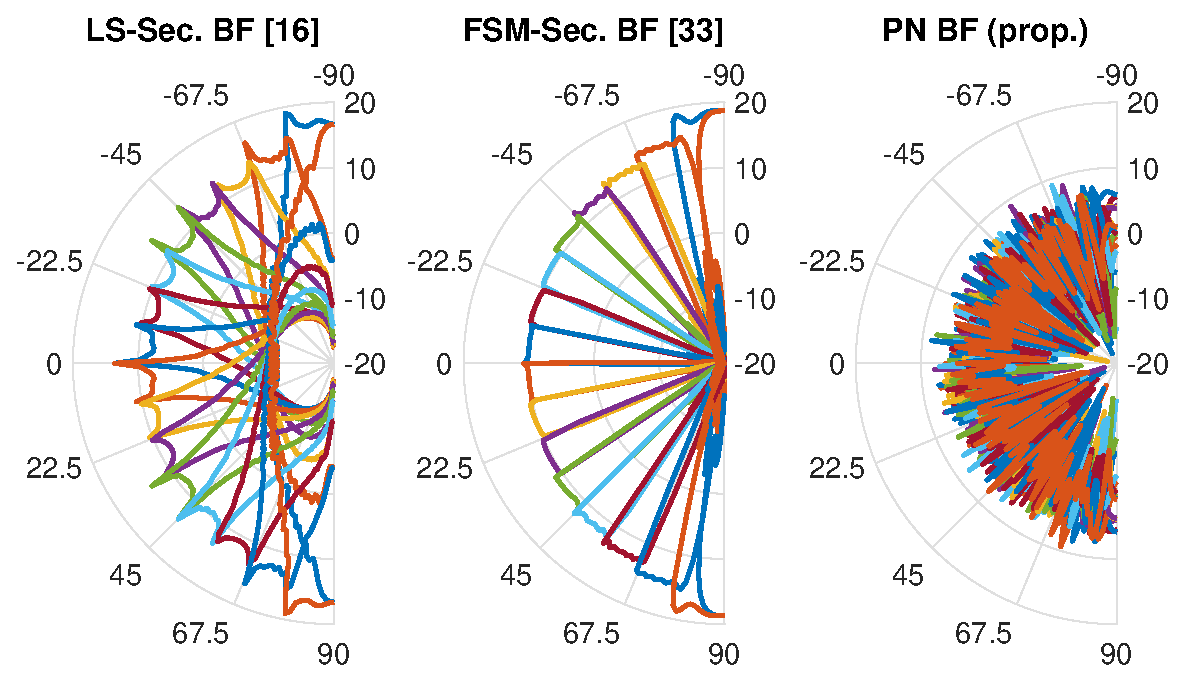
\includegraphics[width=0.45\textwidth]{figures/beam_pattern.eps}
% \includegraphics[width=0.5\textwidth]{figures/varingPN_for_NeTS}
\end{center}
\vspace{-4mm}
\caption{Beam pattern of two sector beam designs \cite{6847111,array_textbook} with $M_{\text{T}}=16$ transmit sectors and one realization of the proposed PN beam. In the polarplot, the $r$-axis refers to the gain in dB and the angular axis refers to steering angle in degree and all pattern refer to $N_{\tx} = 128$ ULA.}
\vspace{-4mm}
\label{fig:beam_pattern}
\end{figure}

%%%%%%%%%%%%%%%%%%%%%%%%%%%%%%%%%%%%%%%%%%%%%%%%%%%%%%%%%%%%%%
% 
%               Section: Numerical results
%
%%%%%%%%%%%%%%%%%%%%%%%%%%%%%%%%%%%%%%%%%%%%%%%%%%%%%%%%%%%%%
\subsection{Performance in simplified SV channel model}
The miss detection rate of the proposed approach in initial discovery is shown in Fig.~\ref{fig:detection_theo_vs_sim} and it verified the theoretical expressions (\ref{eq:PMD_w_STO}). We have the following findings. Firstly, the lack of perfect timing synchronization introduces around 3 dB sensitivity loss as shown between the blue circled curve and red solid curve. However, it is unavoidable in practice systems. Secondly, less than 3 dB sensitivity loss occur when $\pm$5 ppm CFO is present, as shown between the blue dashed curve and green dashed-and-dotted curve. Finally, the practical TO ($\leq10\mu$s) is noncritical as shown in red solid and blue dashed curves. But when TO is large enough to causes transmitter and receiver burst beamforming window mismatch, e.g., 17 $\mu$s TO, severe sensitivity loss is introduces as shown in grey dotted curves. In summary, simulation verifies the conclusions from Section~\ref{sec:cell_discovery} that practical initial synchronization error introduce up to few dB sensitivity loss as compared to ideal scenario. The comparison among proposed and benchmark initial discovery approaches is presented. Although common sense may doubt the efficacy of the proposed approach since there is no significant angular gain in beam pattern, i.e., Fig.~\ref{fig:beam_pattern}, the results show there is marginal difference among the proposed approach and benchmark. This is because the proposed scheme collects spread signal energy over all $M$ SS bursts and gives equivalent measurement as directional approach where energy collection is occur when sector beams align with true propagation directions.

% The comparison among proposed and benchmark initial discovery approaches is shown in Fig.~\ref{fig:detection_comparison}. Note that benchmark approach suffer from synchronization error in a same way as the proposed scheme and the comparison is based on $\pm$5ppm CFO and $10\mu$s timing offset. We have two findings. Firstly, although common sense may doubt the efficacy of the proposed approach since there is no significant angular gain in beam pattern, i.e., Fig.~\ref{fig:beam_pattern}, the results show there is marginal difference among the proposed approach and benchmark. This is because the proposed scheme collects spread signal energy over all $M$ SS bursts and gives equivalent measurement as directional approach where energy collection is occur when sector beams align with true propagation directions. Secondly, the proposed scheme is irrelevant to multipath level $L$ in initial discovery as shown in Section~\ref{sec:cell_discovery}. The directional IA suffers from increased $L$, since with large $L$, the power burst when sector beam is aligned with one propagation direction reduces. In summary, there is marginal difference, if any, in the initial discovery stage, Next, we show the initial BF training performance when system reuses the received SS burst signals for processing.

% cell discovery performance with various initial CFO and array size are shown in . The presence of CFO reduces the cross-correlation output and effectively reduces detection performance. Both PN beam and directional beams degrades according to proposition I and II. However, the cell discovery performance is relatively robust to mild CFO and with practical hardware specification, only marginal coverage loss is observed. When larger number of bursts are used, the covarage is also improved as in proposition I and II.


\begin{figure}
\begin{center}
\includegraphics[width=0.52\textwidth]{figures/alignment_rate_final}
% \includegraphics[width=0.5\textwidth]{figures/varingPN_for_NeTS}
\end{center}
\vspace{-4mm}
\caption{Simulated (Sim.) and theoretical (Theo.) results of the miss detection rate of the proposed initial discovery with various synchronization errors. The discovery rate of the directional initial access is also included as benchmark and both LS-Sec. and FSM-Sec. are used as sector beams. The BS and UE have $N_{\tx} = 128$ and $N_{\rx}=32$ ULA and SV channel has $L=2$ multipaths.}
\vspace{-4mm}
\label{fig:detection_theo_vs_sim}
\end{figure}

% \begin{figure}
% \begin{center}
% 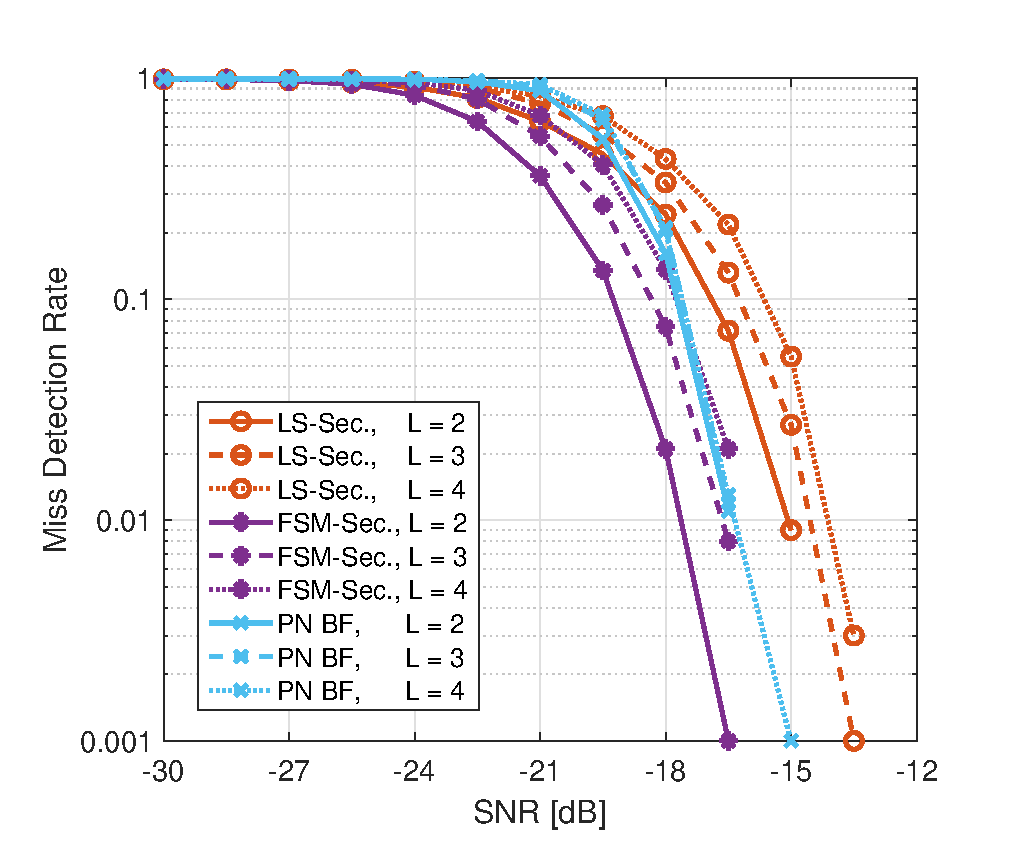
\includegraphics[width=0.5\textwidth]{figures/detection_approach_comp_change_L}
% % \includegraphics[width=0.5\textwidth]{figures/varingPN_for_NeTS}
% \end{center}
% \vspace{-2mm}
% \caption{Simulated results of miss detection rate of the proposed and benchmark initial discovery with two sector beam pattern designs \cite{6847111,array_textbook} in various channel multipaths. The BS has $N_{\tx} = 128$ ULA and UE has $N_{\rx}=32$ ULA. BS and UE have CFO = 5ppm and STO = 10$\mu$s.}
% \vspace{-2mm}
% \label{fig:detection_comparison}
% \end{figure}

%%%%%%%%%%%%%%%%%%%%%%%%%%%%%%%%%%%%%%%%%%%%%%%%%%%%%%%%%%%%%%
% 
%               Section: Numerical results
%
%%%%%%%%%%%%%%%%%%%%%%%%%%%%%%%%%%%%%%%%%%%%%%%%%%%%%%%%%%%%%

The beam training performance of the proposed BF training algorithm in LOS is presented in Fig.~\ref{fig:CRLB}. The simulation is conducted with assumption that SS burst has been detected and ideal timing acquisition is reached. For tractability, the channel parameter the channel parameter and frequency offsets, $\boldsymbol{\xi}$ and PN beamformer $\{\mathbf{v}_m,\mathbf{w}_m\}$ are deterministic in evaluating CRLB. A same pseudorandom setting is used in both simulation has CRLB evaluation. The performance metrics are the residual mean square error defined by $\text{RMSE}_{\text{AoA}} = \sqrt{\mathbb{E}|\hat{\phi}_1-\phi_1|^2}$ and $\text{RMSE}_{\text{AoD}} = \sqrt{\mathbb{E}|\hat{\theta}_1-\theta_1|^2}$. We have the following findings. Firstly, when the refinement steps are used, the proposed algorithm reaches CRLB in high SNR regime. Secondly, the coarse estimation in high SNR has a compromised performance as compared to CRLB. However coarse estimation has accuracy adequate enough for beam steering since RMSE is order of magnitude lower than $3$ dB beam-width, i.e., $0.29\pi/N_{\tx}$ and $0.29\pi/N_{\rx}$ \color{red}[ref]\color{black}. Finally, Fig.~\ref{fig:detection_theo_vs_sim} and \ref{fig:CRLB} reveal that in certain SNR region ($-15$ to $-7.5$ dB) reliable detection occurs but beam training performance is poor. Admittedly, this implies to a compromised experience for UEs in the cell edge which worth further investigation\footnote{It is worth noting that UEs in cell edge are likely to be in NLOS environment, which makes situation more complicated to analyze.}. 


\begin{figure}
\begin{center}
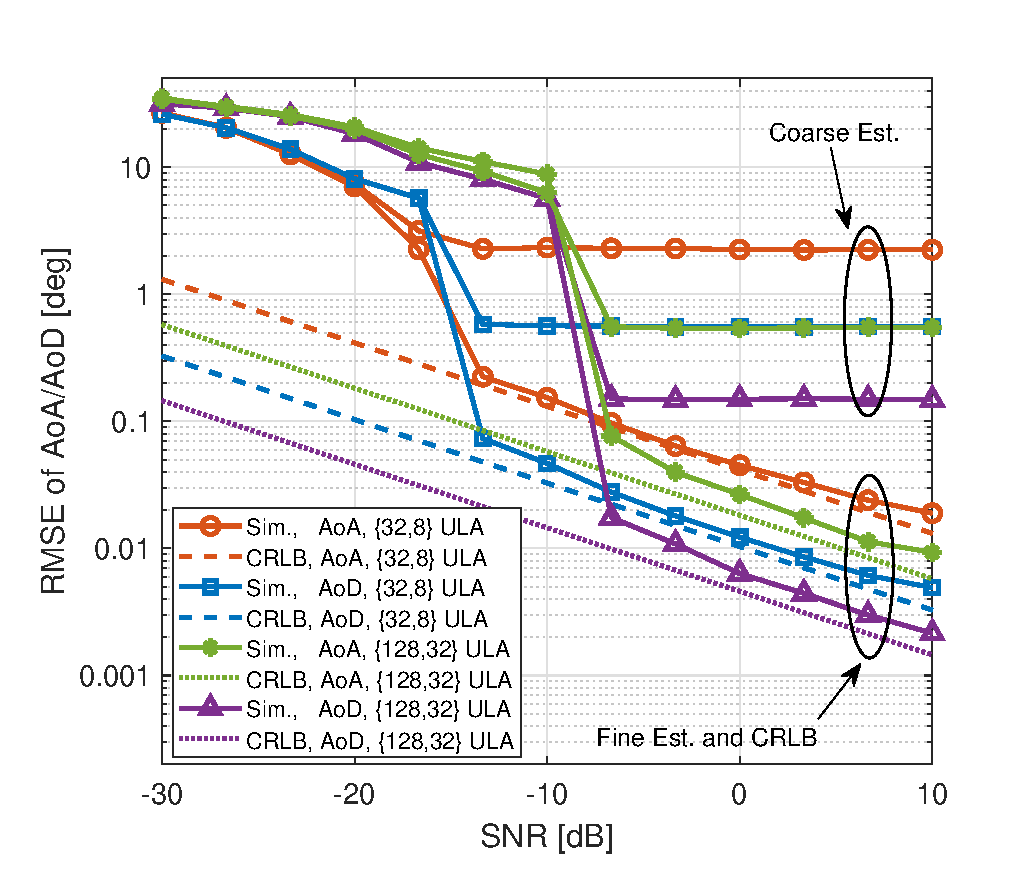
\includegraphics[width=0.48\textwidth]{figures/BF_training_sim_CRLB_new}
% \includegraphics[width=0.5\textwidth]{figures/varingPN_for_NeTS}
\end{center}
\vspace{-4mm}
\caption{Simulated results of the proposed algorithm, with and without refinement steps, and theoretical bound of RMSE of AoA/AoD estimation in LOS. Both array geometry setting, $\{N_{\tx},N_{\rx}\} = \{32,8\}$ ULA and $\{N_{\tx},N_{\rx}\} = \{128,32\}$ ULA are evaluated. System has 5ppm CFO.}
\vspace{-4mm}
\label{fig:CRLB}
\end{figure}


%%%%%%%%%%%%%%%%%%%%%%%%%%%%%%%%%%%%%%%%%%%%%%%%%%%%%%%%%%%%%%
% 
%               Section: Numerical results
%
%%%%%%%%%%%%%%%%%%%%%%%%%%%%%%%%%%%%%%%%%%%%%%%%%%%%%%%%%%%%%
\subsection{Performance in QuaDRiGa channel simulator}
\label{sec:realistic_sim}

Fig.~\ref{fig:overall_evaluation} (a) illustrated the network setting in QuaDRiGa. We consider the performance typical UEs distributed in two planes, one is with moderate distance and the other has larger distance that corresponds to the edge of mmW pico cell. We have the following findings in Fig.~\ref{fig:overall_evaluation} (b) in terms of post training SNR. 
%
Firstly, the proposed approach is comparable with DIA with $N_{\text{train}} = 2$ CSI-RS. In fact, in LOS environment, both approaches are close to beam steering towards true LOS path. Although the SNR seems excessively high in LOS, system designer can simply reduce transmit power to save power.
%
Secondly, DIA with up to $N_{\text{train}} = 2$ CSI-RS has compromised SNR performance. Their drawbacks are intuitive because wide sounding sector beam fails to extract precise angle information. Their SNR degradation versus other curves are more critical in LOS environment since best SNR is captured by perfectly aligning beam with LOS path.
%
Thirdly, although the proposed approach is tailored for sparse channel and phase measurement error due to CFO, it is robust in NLOS scenario when channel sparsity is compromised and practical phase noise occur. Admittedly, it has certain chance to completely fail when NLOS UEs are distributed in the second plane, the counterpart from DIA and CSI-RS cannot do much better jobs. In fact, the proposed approach still have high probability to reach above $0$ dB post-training beam steering SNR than state-of-the-art.

The overhead and initial access latency saving is significant when system does not require CSI-RS as shown in Fig.~\ref{fig:overall_evaluation} (c). As explained in Section~\ref{sec:comparison_analysis}, longer access latency when more UEs are in the network since system need to schedule the CSI-RS resource to those UEs. Increasing the density of CSI-RS effectively reduce latency but it is with the cost of increased overhead. The proposed approach relies on advanced signal processing to digitally conduct beam training and avoids requesting CSI-RS in initial access. It results in a initial access latency saving by two order of magnitudes.



% \begin{figure*}
% \begin{center}
% \includegraphics[width=0.5\textwidth]{figures/alignment_rate_sector}
% % \includegraphics[width=0.5\textwidth]{figures/varingPN_for_NeTS}
% \end{center}
% \vspace{-4mm}
% \caption{Mis-alignment probability after signal processing of SS bursts. System has 5ppm CFO.}
% \vspace{-4mm}
% \label{fig:alignment_prob}
% \end{figure*}

\begin{figure*}[htp]
% \centering
\begin{tabular}{p{6.7cm}p{12.5cm}}
\subfloat[Network illustration where a UE is randomly distributed in the horizontal plane with height of UE within 20 meters. ]{%
  \includegraphics[clip,width=0.65\columnwidth]{figures/network_setting.pdf}%
} &
\multirow{-6}[15]{*}{\subfloat[The CDF of post-training beam steering SNR in the data phase. For the DIA, different number of CSI-RS $N_{\text{train}}$ are considered. The SNR distribution corresponding to beam steering towards true LOS path (when existing) is also included as benchmark. The miss detection rates are included in each plots.]{%
  \includegraphics[clip,width=1.15\columnwidth]{figures/ALL_SNR_CDF}%
}}\\
\subfloat[Access latency versus overhead according to model (\ref{eq:latency}) and (\ref{eq:overhead}) with different number of UEs that share the scheduled CSI-RS. $P_{\text{MD}}$ is 0.04.]{%
  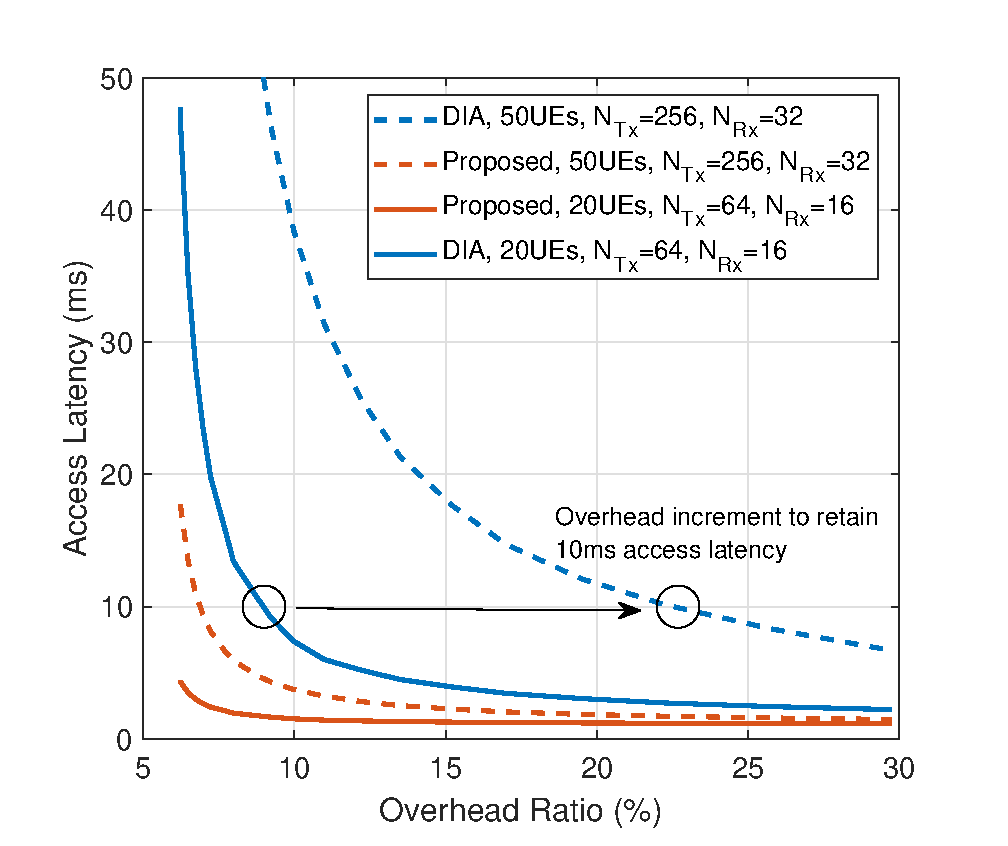
\includegraphics[clip,width=0.73\columnwidth]{figures/latency_vs_OH}%
}
\end{tabular}
\vspace{0mm}
\caption{Initial access and beam training of proposed and benchmark approaches performance in a realistic 3D outdoor UMi network using QuaDRiGa \cite{6758357} with mmMAGIC channel model \cite{mmMAGIC_model}. The trade off between post-training SNR in the data phase, required overhead, and access latency are also studied.}
\label{fig:overall_evaluation}
\end{figure*}


\subsection{Baseband processing requirements}
Using the parameter in Table~\ref{tab:simulation_setting}, and a conservative assumption that algorithm re-run every $\TSS = 20$ ms, the proposed approach requires 0.27 Giga-operations per second (GOPS) for initial discovery and BF training with high-accuracy. Although exact value of required processing power varies with design, the estimated operation numbers implies that the proposed approach is computational friendly considering the state-of-the-art field-programmable gate array (FPGA) with $\geq$0.1GOPS/mW power efficiency [ref].


% \begin{figure}
% \begin{center}
% 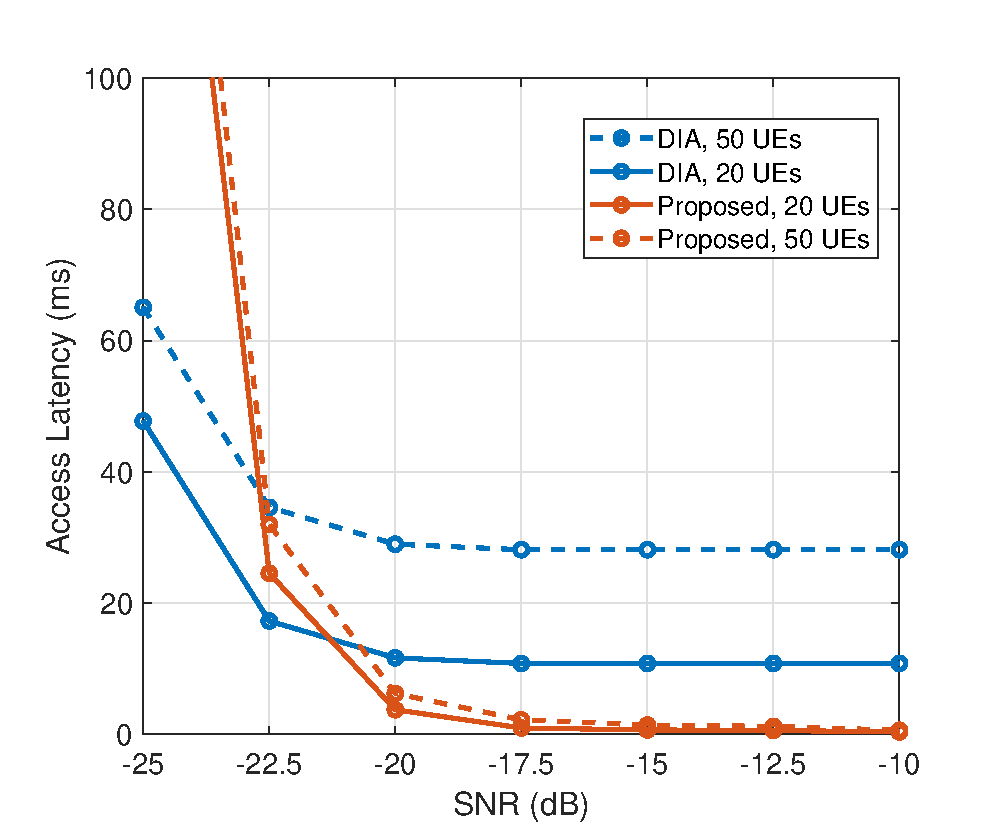
\includegraphics[width=0.5\textwidth]{figures/latency_vs_SNR}
% % \includegraphics[width=0.5\textwidth]{figures/varingPN_for_NeTS}
% \end{center}
% \vspace{-4mm}
% \caption{Access latency as function of number of UEs served by a mmW BS.}
% \vspace{-4mm}
% \label{fig:latency}
% \end{figure}

% \begin{figure}
% \begin{center}
% 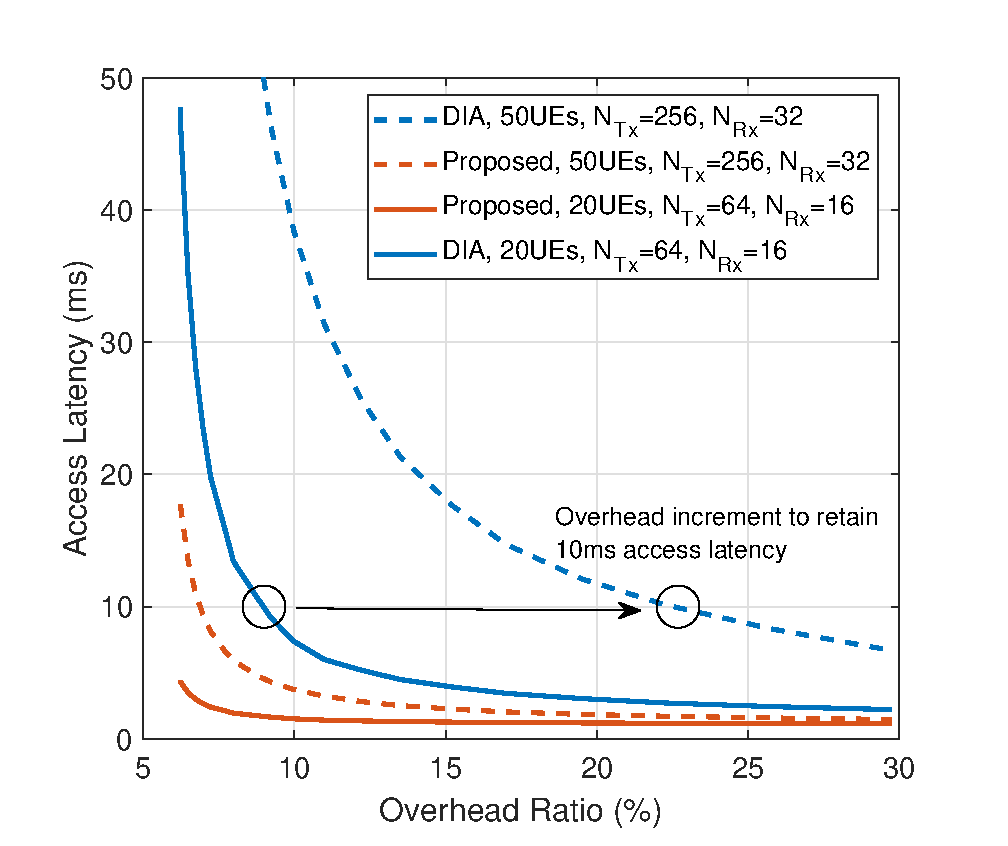
\includegraphics[width=0.5\textwidth]{figures/latency_vs_OH}
% % \includegraphics[width=0.5\textwidth]{figures/varingPN_for_NeTS}
% \end{center}
% \vspace{-4mm}
% \caption{Access latency as function of number of UEs served by a mmW BS.}
% \vspace{-4mm}
% \label{fig:overhead}
% \end{figure}


%%%%%%%%%%%%%%%%%%%%%%%%%%%%%%%%%%%%%%%%%%%%%%%%%%%%%%%%%%%%%%
%  
%               Section: conclusion
%
%%%%%%%%%%%%%%%%%%%%%%%%%%%%%%%%%%%%%%%%%%%%%%%%%%%%%%%%%%%%%
\section{Discussion on Open issues}
\label{sec:discussion}
In this section, we discuss relevant issues in practical implementing compressive IA and beam training. 

\textit{Required a-priori knowledge:} Firstly, this work assumes coarse timing is available. The system is yet to be studied when timing is completely unknown, i.e., no a-priori range information of $\STO$ in (\ref{eq:rx_signal_raw}), and possibly SS burst index misalignment occurs. Secondly, the compressive approach requires precise information of the array geometry and the sounding codebook of both BS and UE. It raise challenge in communication protocol design to effectively incorporate different physical array arrangement. The on-line array geometry learning can be an attractive approach for future investigation. 
% Finally, the transmitter and receiver sounding codebook needs to known as a-priori. Admittedly, it increases challenge of implementing since commonly UE and BS assumes local knowledge of the IA codebook.

\textit{Channel sparsity:} The efficacy of compressive approach is affected to the sparsity level in AoA, AoD, and delay. Although sparsity is endorsed by various mmW channel measurement campaign, and urban NLOS is tested in this work, severely unfavorable rich scattering situation may occurs, e,g, there are up to $L=20$ multipath cluster in the 3GPP specified mmW channel \cite{3GPP_model}. It is important for system to flexibly handle when channel loses sparsity.

\textit{Array architecture:} In this work, we focus on the scenario where UE uses a single RF-chain to process a single stream of IA signals. This facilitates other RF-chains, if available in BS or UE, to operate in the band of data communication without pausing in IA. Since \cite{7161389} shows that the hybrid analog and digital array and fully digital array are advantageous In DIA, it would be interesting to investigate whether this conclusion applies to the compressive IA and beam training approach. 

\textit{MIMO Multiplexing:} The proposed beam training is compatible with MIMO multiplexing in the hybrid array architecture. In fact, designs \cite{7160780,7914742} rely on each RF-chain and corresponding analog beamformer to provide maximum post-BF SNR and uses the digital baseband to handle multi-beam interference. Although its optimality is challenged by recent works \cite{8323164}, it is yet to study whether extra performance is worthwhile with cost of more sophisticated channel training.

\textit{Phase coherency:} To date, there is no coherent CS-based beam training prototype reported in mmW band. The only notable prototype \cite{7146023} operates in 8GHz and two phased array are synchronized by cabled reference clock. Except the CFO as emphasized in this work, the phase noise can also severely degrades coherency among channel observations. Their detrimental impact become more severe with increased carrier frequency , e.g., 73, 90, 140GHz and above \cite{DBLP_1811_03269}. Proper phase noise compensation as well as non-coherent CS-based beam training \cite{Rasekh_noncoherentCS_ACM_2017,UCSB_noncoherentCS_arxiv_1801,Hassanieh:2018:FMW:3230543.3230581} are naturally immune to phase error is worth investigating.






%%%%%%%%%%%%%%%%%%%%%%%%%%%%%%%%%%%%%%%%%%%%%%%%%%%%%%%%%%%%%%
%  
% 							Section: conclusion
%
%%%%%%%%%%%%%%%%%%%%%%%%%%%%%%%%%%%%%%%%%%%%%%%%%%%%%%%%%%%%%
\section{Conclusions}
\label{sec:Conclusion}
In this work, quasi-omni pseudorandom sounding beam is proposed for the mmW initial access, synchronization, and beam training. We design associated signal processing algorithm tailored for 5G-NR frame structure and the proposed sounding beam. We provide theoretical analysis of cell discovery rate and beam training performance and evaluated with simulation using the mmW hardware and urban channel model endorsed by measurements. The results showcases that the proposed approach is comparable with the state-of-the-art directional cell search in cell discovery performance, but significantly more accurate in the initial beam training. This advantage holds true across different propagation condition (LOS/NLOS) and UE-BS distance. Due to the saving of additional radio resource (CSI-RS) for beam refinement, the proposed approach reduces up to two order of magnitude access latency versus the directional initial access when the same signaling overhead and post-training beam steering SNR are targeted.

The MATLAB simulation scripts used in this work are accessible in \cite{hyan_git}.


%%%%%%%%%%%%%%%%%%%%%%%%%%%%%%%%%%%%%%%%%%%%%%%%%%%%%%%%%%%%%%%%%%%%%%%%%%%%%%%
%%%%%%%%%%%%%%%%%%%%%%%%%%%%%%%%%%%%%%%%%%%%%%%%%%%%%%%%%%%%%%%%%%%%%%%%%%%%%%%
\appendix
% \subsection{Nomenclature}
% \label{appendix:nomenclature}
% Notations used in more than one subsections are summarized in the Table~\ref{tab:notation}.

% \begin{table}
% \caption{Nomenclature}
% \centering
% \begin{tabular}{|c|c|c|}
% \hline 
% Symbol & Dim. &Explainations\tabularnewline
% \hline 
% \hline 
% % Carrier Frequency & $f_c = 28$ GHz\tabularnewline
% % \hline 
% $N_{\tx}$, $N_{\rx}$ & $\mathbb{Z}$ & Number of antenna in BS and UE\tabularnewline
% \hline 
% $p$, $P$ & - & Index and total number of subcarriers\tabularnewline
% $m$, $M$ & - & Index and total number of SS bursts\tabularnewline
% \hline 
% $\Ts$ & - & Sample duration\tabularnewline 
% $\Tb,\Nb$ & - & SS burst duration and samples\tabularnewline
% $\TSS$ & - & Period of SS bursts\tabularnewline
% $\Nc$ & $\mathbb{Z}$ & Max. excess delay taps and length of CP\tabularnewline
% $\Ncp$ & $\mathbb{Z}$ & Cyclic-prefix length of OFDM symbols\tabularnewline
% \hline 
% $\Delta f$ & - & Initial CFO in UE (absolute value) \tabularnewline
% $\epsilon_{\text{F}}$ & - & Initial CFO in UE (normalized with $\Ts$)\tabularnewline
% $\epsilon_{\text{T}}$ & $\mathbb{Z}$ & Initial TO in UE (number of sample) \tabularnewline
% \hline 
% $\mathbf{H}[d]$ & $\mathbb{C}^{N_{\rx} \times N_{\tx}}$ & MIMO channel at $d$-th delay sample\tabularnewline
% $\mathbf{a}_{\tx}\left(\theta\right)$ & $\mathbb{C}^{N_{\tx}}$ & Spatial responses of BS ULA\tabularnewline
% $\mathbf{a}_{\rx}\left(\phi\right)$ & $\mathbb{C}^{N_{\rx}}$ & Spatial responses of UE ULA
% \tabularnewline
% $l, L$ & - & Index and total number of multipaths \tabularnewline
% $\phi_l,\theta_l$ & - &AoA/AoD of $l$-th multipath  \tabularnewline
% $g_l$ & - & Complex channel gain of $l$-th multipath  \tabularnewline
% $\alpha_l, \beta_l$ & - & Real and imaginary parts of $g_l$  \tabularnewline
% $\tau_l$ & - & Exces. Delay of $l$-th multipath  \tabularnewline
% \hline 
% $\mathbf{s}, \tilde{\mathbf{s}}$ & $\mathbb{C}^{P}$ & F/T domain PSS vector\tabularnewline
% $\tilde{s}[n]$ & - & T-domain. PSS sequence\tabularnewline
% $\mathbf{v}_m, \mathbf{w}_m$ & $\mathbb{C}^{N_{\tx}},\mathbb{C}^{N_{\rx}}$ & RF precoder/combiner of the $m$-th burst\tabularnewline
% $z[n]$ & - & AWGN sequence\tabularnewline
% $\mathbf{z}_m$ & $\mathbb{C}^{P}$ & AWGN vector at $m$-th burst \tabularnewline
% $\mathbf{y}_m$ & $\mathbb{C}^{P}$ & Received OFDM symbols at $m$-th burst \tabularnewline
% $\sigman^2$ & $$ & AWGN power \tabularnewline
% \hline 
% \multicolumn{3}{|c|}{Initial discovery (detection)}\tabularnewline
% \hline
% $P^{\star}_{\text{FA}}$ & - & Target FA prob. in initial discovery \tabularnewline
% $P_{\text{MD,PT}}$ & - & MD prob. with perfect timing  \tabularnewline
% $P_{\text{MD,NT}}$ & - & MD prob when timing is unknown \tabularnewline
% $\gamma_{\text{PT}}, \eta_{\text{PT}}$ & - & Detection stat. and TH w/ perfect timing\tabularnewline
% $\gamma_{\text{NT}}, \eta_{\text{NT}}$ & - & Detection stat. and TH w/ unknown timing\tabularnewline
% $P_{\text{TO}}$ & - & Prob. of acquisiting perfect timing \tabularnewline
% \hline 
% \multicolumn{3}{|c|}{Initial beamforming traning (estimation)}\tabularnewline
% \hline
% $\boldsymbol{\xi}$ & $\mathbb{R}^{5L+1}$ & Parameters to estimate in BF training \tabularnewline
% $\Gd$ & - & Parameter grid in delay est. \tabularnewline
% $\Gt$, $\Gr$ & - & Parameter grid in AoA/AoD est. \tabularnewline
% $\mathbf{Q}$ & $\mathbb{C}^{P\times P}$ & ICI matrix in BF training \tabularnewline
% \hline
% \multicolumn{3}{|c|}{Latency and Overhead}\tabularnewline
% \hline
% $\text{OH}$ & - & Overhead ratio of IA signals \tabularnewline
% \hline 
% \end{tabular}
% \label{tab:notation}
% \end{table}


%%%%%%%%%%%%%%%%%%%%%%%%%%%%%%%%%%%%%%%%%%%%%%%%%%%%%%%%%%%%%%
%
%                        Appendix detection performance
%
%%%%%%%%%%%%%%%%%%%%%%%%%%%%%%%%%%%%%%%%%%%%%%%%%%%%%%%%%%%%%%

\subsection{Initial discovery performance}
\label{appendix:detection_derivation_wo_STO}
The noise after autocorrelation $\tilde{z}[n] = \sum_{n=0}^{P-1}(\mathbf{w}^{\hermitian}[n+p]\mathbf{z}[n+p])s^{*}[p]$ is zero mean complex white Gaussian process with variance $\sigman^2/P$. Therefore $|\tilde{z}[n]|^2$ is Chi-Square random variable with degree-of-freedom 2, mean $\sigman^2/P$, and variance $\sigman^4/P^2$. The detection statistic under $\mathcal{H}_0$ is denoted as $\gamma_{\text{PT},0}$. It is the square-sum of $\Nc M$ realizations of $\tilde{z}[n]$ before divided by $M$ and central limit theory (CLT) applies. The mean and standard deviation of $\gamma_{\text{PT},0}$ are  $\mu_{\text{PT},0} =  \Nc\sigman^2/P$ and $\sigma_{\text{PT},0} =  \sqrt{\Nc\sigman^4/(P^2M)}$, respectively. As a result, the optimal detection threshold that reaches target false alarm rate $P^{\star}_{\text{FA}}$ is as (\ref{eq:TH_w_STO}). 
Similarly, the detection statistic under $\mathcal{H}_0$ is denoted as $\gamma_{\text{NT},0}$. It is the maximum operation with degree of freedom $\epsilon_{\text{T,max}}$ of $\gamma_{\text{PT},0}$. With large $\epsilon_{\text{T,max}}$, $\gamma_{\text{NT},0}$ follows extreme value distribution, \textit{Gumbel Distribution}, where the mean and standard deviation are 
$\mu_{\text{NT},0} = \mu_{\text{PT},0}+\sigma_{\text{PT},0}\Q^{-1}\left(1/\epsilon_{\text{T,max}}\right) \text{ and }$ and $\sigma_{\text{NT},0} = \sigma_{\text{PT},0}/\Q^{-1}\left(1/\epsilon_{\text{T,max}}\right)$, respectively.
% \cite{extreme_dist}.
Using its inverse cumulative distribution function, the optimal detection threshold is
$\eta^{\star}_{\text{NT}} = \mu_{\text{NT},0} - (\sqrt{6}\pi)\sigma_{\text{NT},0} \ln\left(-\ln\left(1-P^{\star}_{\text{FA}}\right)\right)$. It gives (\ref{eq:TH_w_STO}) using expressions of $\mu_{\text{NT},0}$, $\sigma_{\text{NT},0}$ and $\sqrt{6}/\pi\approx 0.78$.


% \begin{align}
% \eta^{\star}_{\text{PT}} = \frac{\Nc \sigman^2}{P} +\frac{\sqrt{\Nc}\sigman^2}{\sqrt{M}P}Q^{-1}\left(P^{\star}_{\text{FA}}\right)
% \end{align}

With perfect synchronization, the detection statistic under $\mathcal{H}_1$ is denoted as $\gamma_{\text{PT},1}$ and it is the sum of signal energy and noise energy $\gamma_{\text{PT},0}$. Therefore
% \begin{align}
% \begin{split}
% \gamma_{\text{PT},1} = &\frac{1}{MLN_{\tx}N_{\rx}}\sum_{m=1}^{M}\sum_{l=0}^{L}\left|\tilde{g}_{m,l}\sum_{n=1}^{P}|s[n]|^2\right|^2 + \gamma_{\text{PT},0}\\
% =& \frac{1}{MLN_{\tx}N_{\rx}}\sum_{m=1}^{M}\sum_{l=0}^{L}\left|\tilde{g}_{m,l}\right|^2 + \gamma_{\text{PT},0}
% \end{split}
% \end{align}
$\gamma_{\text{PT},1} = (\sum_{m=1}^{M}\sum_{l=0}^{L}|\tilde{g}_{m,l}\sum_{n=1}^{P}|s[n]|^2|^2)/(MN_{\tx}N_{\rx}) + \gamma_{\text{PT},0}
= \sum_{m=1}^{M}\zeta_m/M + \gamma_{\text{PT},0}$
where $\zeta_m=\sum_{l=0}^{L}|g_l\mathbf{w}^{\hermitian}_m\mathbf{a}_{\rx}(\phi_l)\mathbf{a}^{\hermitian}_{\tx}(\theta_l)\mathbf{v}_m|^2/(N_{\tx}N_{\rx})$. Using the fact that $\zeta_m$ are mutually independent due to independent $\mathbf{v}_m$ and $\mathbf{w}_m$, the mean of $\zeta_m$ is $\mathbb{E}(\zeta_{m}) = \sum_{l=1}^{L}\left|g_l\right|^2\mathbb{E}\left|\mathbf{w}^{\hermitian}_m\mathbf{a}_{\rx}(\phi_l)\right|^2/N_{\tx}\mathbb{E}\left|\mathbf{a}^{\hermitian}_{\tx}(\theta_l)\mathbf{v}_m\right|^2/N_{\rx} = \sigma_{\text{g}}^2$
% \begin{align}
% \begin{split}
% \mathbb{E}(\zeta_{m,l}) = &\mathbb{E}\left|g_l\right|^2\frac{\mathbb{E}\left|\mathbf{w}^{\hermitian}_m\mathbf{a}_{\rx}(\phi_l)\right|^2}{N_{\tx}}\frac{\mathbb{E}\left|\mathbf{a}^{\hermitian}_{\tx}(\theta_l)\mathbf{v}_m\right|^2}{N_{\rx}} = \sigma_{\text{g}}^2
% \end{split}
% \end{align}
% due to the mutual independence among elements of $\mathbf{w}_m$ and $\mathbf{v}_m$. 
The variance of $\zeta_m$ is
$\var(\zeta_{m}) = \sum_{l=1}^{L}\left|g_l\right|^4\mathbb{E}\left|\mathbf{w}^{\hermitian}_m\mathbf{a}_{\rx}(\phi_l)\right|^4/N^2_{\tx}\mathbb{E}\left|\mathbf{a}^{\hermitian}_{\tx}(\theta_l)\mathbf{v}_m\right|^4/N^2_{\rx}-\sigma_{\text{g}}^4
=\sigma_{\text{g}}^4\left(2-\frac{1}{N_{\tx}}\right)\left(2-\frac{1}{N_{\rx}}\right)-\sigma_{\text{g}}^4 \approx 3\sigma_{\text{g}}^4$
% \begin{align}
% \begin{split}
% \text{var}(\zeta_{m,l}) = &\mathbb{E}\left|g_l\right|^4\frac{\mathbb{E}\left|\mathbf{w}^{\hermitian}_m\mathbf{a}_{\rx}(\phi_l)\right|^4}{N^2_{\tx}}\frac{\mathbb{E}\left|\mathbf{a}^{\hermitian}_{\tx}(\theta_l)\mathbf{v}_m\right|^4}{N^2_{\rx}}-\sigma_{\text{g}}^4\\
% =&3\sigma_{\text{g}}^4\left(2-\frac{1}{N_{\tx}}\right)\left(2-\frac{1}{N_{\rx}}\right)-\sigma_{\text{g}}^4 \approx 11\sigma_{\text{g}}^4
% \end{split}
% \end{align}
and approximation holds true when antenna array size $N_{\rx}$ and $N_{\tx}$ are large.
Therefore, according to CLT $\gamma_{\text{PT},1}$ is Gaussian distributed with mean and variance
$\mathbb{E}(\gamma_{\text{PT},1}) = \sigma_{\text{g}}^2 + \mu_{\text{PT},0}$ and $\var(\gamma_{\text{PT},1}) =  3\sigma_{\text{g}}^4/M + \sigma^2_{\text{PT},0}.$
The miss detection probability 
$P_{\text{MD,PT}} = \Q[(\mathbb{E}(\gamma_{\text{PT},1}) - \eta_{\text{PT}})/\sqrt{\var(\gamma_{\text{PT},1})}]$
reduces to (\ref{eq:PMD_w_STO}) after plug-in the expression of $\mathbb{E}(\gamma_{\text{PT},1})$ and $\var(\gamma_{\text{PT},1})$, expression of $\eta^{\star}_{\text{PT}}$ in (\ref{eq:TH_w_STO}), and definition of SNR.
%%%%%%%%%%%%%%%%%%%%%%%%%%%%%%%%%%%%%%%%%%%%%%%%%%%%%%%%%%%%%%
%
%                        Appendix detection performance
%
%%%%%%%%%%%%%%%%%%%%%%%%%%%%%%%%%%%%%%%%%%%%%%%%%%%%%%%%%%%%%%
% \subsection{Detection performance without timing information}
% \label{appendix:detection_derivation_w_STO}



% \begin{align}
% \eta^{\star}_{\text{NT}} = &\frac{\Nc\sigman^2}{P}+\frac{2\Nc\sigman^4}{P^2M}Q^{-1}\left(\frac{1}{\Nb}\right)\\
% & - \frac{2\sqrt{6}\Nc\sigman^4}{\pi P^2M Q^{-1}\left(\frac{1}{\Nb}\right)} \ln\left(\ln\left(P^{\star}_{\text{FA}}\right)\right).
% \end{align}

With no synchronization, the detection statistic under $\mathcal{H}_1$ is denoted as $\gamma_{\text{NT},1}$. The exact distribution of $\gamma_{\text{NT},1}$ is challenging. We make the following approximation to simplify the derivation: 1) the energy of $\gamma_{\text{NT},1}$ corresponding to the true correlation peaks plus noise power; 2) the non-aligned beamformer due to abrupt beamformer change results in independent $\mathbf{v}_m$ and $\mathbf{w}_m$. Based on this assumption, we evaluate distribution of $\gamma_{\text{NT},1}$ by considering the impact of TO and CFO in the following
% \begin{figure*}
% \begin{align}
% \begin{split}
$\gamma_{\text{NT},1} = \frac{1}{MLN_{\tx}N_{\rx}}\sum_{m=1}^{M}\sum_{l=0}^{L}|\tilde{g}^{(1)}_{m,l}\sum_{n_1=1}^{K-1}|s[n_1]|^2e^{j\CFO n_1}+\tilde{g}^{(2)}_{m,l}\sum_{n_2=K}^{P}|s[n_2]|^2e^{j\CFO n_2}|^2 + \gamma_{\text{PT},0}$
% \triangleq& \frac{1}{ML}\sum_{m=1}^{M}\sum_{l=0}^{L}\tilde{\zeta}_{m,l} + \gamma_{\text{PT},0}
% \end{split}
% \label{eq:gamma_nt_1}
% \end{align}
% \hrule
% \end{figure*}
where 
$\tilde{g}^{(1)}_{m,l} =  g_l\mathbf{w}^{\hermitian}_m\mathbf{a}_{\rx}(\phi_l)\mathbf{a}^{\hermitian}_{\tx}(\theta_l)\mathbf{v}_m$ and $\tilde{g}^{(2)}_{m,l} =  g_l\mathbf{w}^{\hermitian}_{m+1}\mathbf{a}_{\rx}(\phi_l)\mathbf{a}^{\hermitian}_{\tx}(\theta_l)\mathbf{v}_m$
are the post-beamforming channel gain due to partially overlapped burst window in BS and UE. In other word, $K$ follows (\ref{eq:define_gain_split_K}) and $n_1\in [1,K-1]$ and $n_2\in [K,P]$ are the sample window with $K$ represents the abrupt change in beamformer. Based on the assumption of independent $\mathbf{w}_m$ and $\mathbf{w}_{m+1}$, $\tilde{g}^{(1)}_{m,l}$ it is straightforward to show that $\tilde{g}^{(2)}_{m,l}$ are uncorrelated.
For notational convenience of finding statistic of $\gamma_{\text{NT},1}$, we define $\zeta_{m,l}$ as $
\zeta_{m,l} 
% \approx &\frac{1}{MLN_{\tx}N_{\rx}}\sum_{m=1}^{M}\sum_{l=0}^{L}\bigg|\tilde{g}^{(1)}_{m,l}\sum_{n_1=1}^{K-1}|s[n_1]|^2e^{j\CFO n_1}\\
% & + \tilde{g}^{(2)}_{m,l}\sum_{n_2=K}^{P}|s[n_2]|^2e^{j\CFO n_2}\bigg|^2 \\
\triangleq  (|\tilde{g}^{(1)}_{m,l}\frac{1-e^{jK\CFO}}{1-e^{j\CFO }}+ \tilde{g}^{(2)}_{m,l}\frac{1-e^{j(P-K)\CFO}}{1-e^{j\CFO }}|^2)/(N_{\tx}N_{\rx}P^2)$
in $\gamma_{\text{NT},1}$ after simplification with the fact $|s[n]|^2 = 1/P, \forall n\in \mathcal{S}$ as well as $\sum_{n=1}^{K}e^{j\STO n} = (1-e^{jK\CFO})/(1-e^{j\CFO})$. The mean of $\zeta_{m,l}$ is $\mathbb{E}\left(\zeta_{m,l}\right)= \kappa(\CFO,\STO)\sigma_{\text{g}}^2$ after plug-in definition in (\ref{eq:kappa_SNR_degradation}).
% Therefore, the best scenario is $K=0$ which corresponds to realization that in UE uses the $m$-th beamformer when receiving signal from the $m$-th burst from BS. The worst scenario is $K=P/2$ which corresponds to realization that in UE uses the $m$-th beamformer to received first $P/2$ sample and $m+1$-th beamformerwhen to receiving the rest of $P/2$ samples of PSS in the $m$-th burst.
The variance of $\zeta_{m,l}$ is $\var\left(\zeta_{m,l}\right) \approx  2\sigma^4_{\text{g}}\zeta^2(\CFO,\STO)$. This is a straightforward extension of derivation and approximation in Appendix~\ref{appendix:detection_derivation_wo_STO}. Using CLT and statistic of $\zeta_{m,l}$, we conclude that $\gamma_{\text{NT},1}$ is Gaussian distributed with mean and variance to be
$\mathbb{E}(\gamma_{\text{NT},1}) = \kappa(\CFO,\STO) \sigma^2_{\text{g}} + \mu_{\text{PT},0}$ and $\text{var}(\gamma_{\text{NT},1}) = 2\sigma^4_{\text{g}}\kappa^2(\CFO,\STO)/M + \sigma^2_{\text{PT},0}$, respectively. The miss detection probability $P_{\text{MD,NT}} = \Q[(\mathbb{E}(\gamma_{\text{NT},1}) - \eta^{\star}_{\text{NT}})/\sqrt{\var(\gamma_{\text{NT},1})}]$ reduces to (\ref{eq:PMD_w_STO}) once one plug-in expressions of $\mu_{\text{NT},0}$, $\eta^{\star}_{\text{NT}}$, and $\gamma_{\text{NT},1}$ and definition of SNR.

% \begin{align}
% P_{\text{MD,NT}} = Q\left(\frac{\left(\frac{2-\Re(e^{j\CFO})}{2-\Re(e^{j\CFO K})}+\frac{2-\Re(e^{j\CFO})}{2-\Re(e^{j\CFO (P-K)})}\right) \sigma^2_{\text{g}} +\frac{2\Nc\sigman^4}{P^2M}Q^{-1}\left(\frac{1}{\Nb}\right) - \frac{2\sqrt{6}\Nc\sigman^4}{\pi P^2M Q^{-1}\left(\frac{1}{\Nb}\right)} \ln\left(\ln\left(P^{\star}_{\text{FA}}\right)\right)}{\sqrt{\frac{11\sigma^4_{\text{g}}}{ML}\left(\frac{2-\Re(e^{j\CFO})}{2-\Re(e^{j\CFO K})}+\frac{2-\Re(e^{j\CFO})}{2-\Re(e^{j\CFO (P-K)})}\right)^2+\sigma^2_{\text{PT},0}}}\right)
% \end{align}

% \begin{table}
% \caption{Nomenclature}
% \centering
% \begin{tabular}{|c|c|}
% \hline 
% Symbol &Explanations\tabularnewline
% \hline 
% \hline 
% % Carrier Frequency & $f_c = 28$ GHz\tabularnewline
% % \hline 
% $p$, $P$ &  Index and total number of subcarriers\tabularnewline
% $m$, $M$ &  Index and total number of SS bursts\tabularnewline
% $l, L$  & Index and total number of multipaths \tabularnewline
% \hline 
% $N_{\tx}$, $N_{\rx}$  & Number of antenna in BS and UE\tabularnewline
% $\Ts$ &  Sample duration of IA signal\tabularnewline 
% $\Tb,\Nb$ &  Duration and sample number in each SS burst\tabularnewline
% $\TSS$ &  Period of SS bursts\tabularnewline
% $T_{\text{R}}$,$T_{\text{r}}$ &  Period and duration of CSI-RS\tabularnewline
% $\Nc$, $\Ncp$ &  Max. excess delay taps and length of CP\tabularnewline
% $N_{\text{train}},N_{\text{U}}$ &  Required CSI-RS and UE number\tabularnewline
% \hline 
% $\Delta f$, $\epsilon_{\text{F}}$ &  CFO in [Hz] and normalized in [rad/samp.] \tabularnewline
% % $\epsilon_{\text{F}}$ &  Initial CFO in UE (normalized with $\Ts$)\tabularnewline
% $\epsilon_{\text{T}}$ &  Initial TO in UE (number of sample) \tabularnewline
% \hline 
% $\mathbf{H}[d]$ & MIMO channel at $d$-th delay sample\tabularnewline
% $\mathbf{a}_{\tx}\left(\theta\right)$, $\mathbf{a}_{\rx}\left(\phi\right)$   & Spatial responses of BS and UE\tabularnewline
% % $\mathbf{a}_{\rx}\left(\phi\right)$  & Spatial responses of UE ULA\tabularnewline
% $\phi_l,\theta_l$, $g_l$, $\tau_l$  &Gain/AoA/AoD/delay of $l$-th multipath  \tabularnewline
% % $g_l$  & Complex channel gain of $l$-th multipath  \tabularnewline
% $\alpha_l, \beta_l$  & Real and imaginary parts of $g_l$  \tabularnewline
% % $\tau_l$  & Exces. Delay of $l$-th multipath  \tabularnewline
% \hline 
% $\mathbf{s}, \tilde{\mathbf{s}}$, $\tilde{s}[n]$ & F/T domain PSS vector and sequence\tabularnewline
% % $\tilde{s}[n]$ &  T-domain. PSS sequence\tabularnewline
% $\mathbf{v}_m, \mathbf{w}_m$ & RF precoder/combiner of the $m$-th burst\tabularnewline
% $z[n]$, $\mathbf{z}_m$, $\sigman^2$ & AWGN sequence, vector, and power\tabularnewline
% % $\mathbf{z}_m$  & AWGN vector at $m$-th burst \tabularnewline
% % $\sigman^2$  & AWGN power \tabularnewline
% \hline 
% \multicolumn{2}{|c|}{Initial discovery (detection)}\tabularnewline
% \hline
% $P^{\star}_{\text{FA}}$ & Target FA prob. in initial discovery \tabularnewline
% $P_{\text{MD,PT}}$, $P_{\text{MD,NT}}$ & MD prob. w/ and w/o perfect timing  \tabularnewline
% % $P_{\text{MD,NT}}$ & MD prob when timing is unknown \tabularnewline
% $\gamma_{\text{PT}}, \eta_{\text{PT}}$ & Detection stat. and TH w/ perfect timing\tabularnewline
% $\gamma_{\text{NT}}, \eta_{\text{NT}}$ & Detection stat. and TH w/ unknown timing\tabularnewline
% % $P_{\text{TO}}$ & Prob. of acquisiting perfect timing \tabularnewline
% \hline 
% \multicolumn{2}{|c|}{Initial beamforming traning (estimation)}\tabularnewline
% \hline
% $\boldsymbol{\xi}$ & Parameters to estimate in BF training \tabularnewline
% % $\Gd$ &  Parameter grid in delay est. \tabularnewline
% $\mathbf{y}_m$  & Received OFDM symbols at $m$-th burst \tabularnewline
% $\mathbf{d}$, $\mathbf{t}$, $\mathbf{r}$ & Vectors with candidates delay/AoA/AoD \tabularnewline
% $\Gd$, $\Gt$, $\Gr$ & Parameter grid in delay/AoA/AoD est. \tabularnewline
% $\mathbf{Q}$, $\mathbf{F}$ & ICI matrix and DFT matrix \tabularnewline

% \hline
% % \multicolumn{2}{|c|}{Latency and Overhead}\tabularnewline
% % \hline
% % $\text{OH}$  & Overhead ratio of IA signals \tabularnewline
% % \hline 
% \end{tabular}
% \label{tab:notation}
% \end{table}
%%%%%%%%%%%%%%%%%%%%%%%%%%%%%%%%%%%%%%%%%%%%%%%%%%%%%%%%%%%%%%
%
%                        Appendix timing acquisition
%
%%%%%%%%%%%%%%%%%%%%%%%%%%%%%%%%%%%%%%%%%%%%%%%%%%%%%%%%%%%%%%
% \subsection{Timing Acquisition performance}
% \label{appendix:timing_sync_derivation}
% \color{red} Need more work here.
% \color{black}

% The distribution of detection statistic $\gamma_0$ under $\mathcal{H}_0$ is found by following steps: 1) post-correlation AWGN follows circular Gaussian distribution $\bar{z}[n]\sim\mathcal{CN}(0,\sigma_n^2/N_{ZC})$. 2) random variable after ``peak-sum'' operation is chi-square distributed with degree of freedom being $M_{burst}$. Its mean and variance is denoted as $\mu_0$ and $\sigma_0^2$, respectively. 3) $\gamma_0$ follows extreme value distribution and its mean and standard deviation is $\mu_0-\sigma_0Q^{-1}(1/N_{burst})$ and $\sigma_0/Q^{-1}(1/N_{burst})$, respectively.

% Next, we consider detection performance with STO. The detection statistic is 
% \begin{align}
% \gamma_1 \triangleq \max_{n} \frac{1}{M_{\text{burst}}}\sum_{m=1}^{M_{\text{burst}}}|p[n]+\bar{z}[n+mN_{\text{burst}}]|^2
% \end{align}

% We make the following approximation
% \begin{align}
% \gamma_1 \approx \max \left\{\frac{1}{M_{\text{burst}}}\sum_{m=1}^{M_{\text{burst}}}|\bar{p}[m]+\bar{z}[m]|^2, \gamma_0\right\}
% \end{align}
% where $\bar{p}[m]$ is true peak sequence defined as 
% \begin{align}
% \bar{p}[m] = \frac{1}{N_{\text{ZC}}}\sum_{m=0}^{N_{ZC}-1}\mathbf{w}^{\hermitian}[n+m]\mathbf{H}^{(\text{t})}\mathbf{v}[n+m-\epsilon_{\text{STO}}]
% \end{align}
% The distribution of detection statistic $\gamma_0$ in hypothesis $\mathcal{H}_1$ is
% \begin{align*}
% \gamma_1 \approx \max \left\{\underbrace{\frac{1}{M_{\text{burst}}}\sum_{m=1}^{M_{\text{burst}}}|\bar{p}[m]+\bar{z}[m]|^2}_{\gamma_{\text{peak}}+\gamma_{\text{n}}}, \gamma_0\right\}
% \end{align*}
% where r.v. $\gamma_n$ represent AWGN power at correlation peaks and r.v. $\gamma_{peak}$ represents power of correlation peaks. To find the distribution of $\gamma_{peak}$, we use central-limit-theory for approximation. Therefore we can evaluate the distribution of r.v. such that $\gamma_1 = \max (\gamma_0,\gamma_{peak}+\gamma_{0})$.
%%%%%%%%%%%%%%%%%%%%%%%%%%%%%%%%%%%%%%%%%%%%%%%%%%%%%%%%%%%%%%
%
%                        Appendix CRLB
%
%%%%%%%%%%%%%%%%%%%%%%%%%%%%%%%%%%%%%%%%%%%%%%%%%%%%%%%%%%%%%%
% \onecolumn
% \subsection{Vectors in refinement}
% \label{app:gradients}
% The partial derivatives of $\mathbf{x}$ over parameters are 
% \begin{align}
% \begin{split}
% \boldsymbol{\nabla}\mathbf{x}_{g} = &\\
% \boldsymbol{\nabla}\mathbf{x}_{\tau} = &\\
% \boldsymbol{\nabla}\mathbf{x}_{\CFO} = &\\
% \boldsymbol{\nabla}\mathbf{x}_{\phi} = &\\
% \boldsymbol{\nabla}\mathbf{x}_{\theta} = &\\
% \end{split}
% \end{align}
% \color{red} To be updated since those equations have overlap with Appendix~\ref{app:CRLB}. I need more thoughts to write in a concise way.\color{black}
%%%%%%%%%%%%%%%%%%%%%%%%%%%%%%%%%%%%%%%%%%%%%%%%%%%%%%%%%%%%%%
%
%                        Appendix CRLB
%
%%%%%%%%%%%%%%%%%%%%%%%%%%%%%%%%%%%%%%%%%%%%%%%%%%%%%%%%%%%%%%
% \onecolumn
\subsection{CRLB of joint estimation problem}
\label{app:CRLB}
\begin{table*}
\caption{Elements of fisher information matrix}
\centering
\def\arraystretch{1.75}%  1 is the default, change whatever you need
\begin{tabular}{|p{0.6cm}|p{7.7cm}|p{0.55cm}|p{7.5cm}|}
\hline 
Symb. & Expressions & Symb. & Expressions\tabularnewline
\hline
$\Phi_{\CFO,\CFO}$ & $\sum_{m=1}^{M}(C_{\text{d2q}}g)\left|\mathbf{w}_m^{\hermitian}{\mathbf{a}}_{\rx}(\phi)\right|^2\left|\mathbf{v}_m^{\hermitian}{\mathbf{a}_{\tx}}(\theta)\right|^2$  & 
$\Phi_{\CFO,\theta}$ & 
$\sum_{m=1}^{M}(C_m g)\left|\mathbf{w}_m^{\hermitian}\mathbf{a}_{\rx}(\phi)\right|^2\Re\left\{\left[\mathbf{v}_m^{\hermitian}\dot{\mathbf{a}_{\tx}}(\theta)\right]\left[\mathbf{v}_m^{\hermitian}{\mathbf{a}_{\tx}}(\theta)\right]\right\}$\tabularnewline
\hline 
$\Phi_{\CFO,\tau}$
& $\Re\left\{\sum_{m=1}^{M}g\left|\mathbf{w}_m^{\hermitian}{\mathbf{a}}_{\rx}(\phi)\right|^2\left|\mathbf{v}_m^{\hermitian}{\mathbf{a}_{\tx}}(\theta)\right|^2\mathbf{f}^{\hermitian}(\tau)\mathbf{F}\dot{\mathbf{Q}}^{\hermitian}_m{\mathbf{Q}}_m\mathbf{F}^{\hermitian}\dot{\mathbf{f}}(\tau)\right\}$
& $\Phi_{\CFO,\alpha} $
& $\sum_{m=1}^{M}\left[C_{\text{dq},m}\Re\left(g\right)\right]\left|\mathbf{w}_m^{\hermitian}{\mathbf{a}}_{\rx}(\phi)\right|^2\left|\mathbf{v}_m^{\hermitian}{\mathbf{a}_{\tx}}(\theta)\right|^2$
\tabularnewline
\hline
$\Phi_{\CFO,\beta}$
& $\sum_{m=1}^{M}\left[C_{\text{dq},m}\Im\left(g\right)\right]\left|\mathbf{w}_m^{\hermitian}{\mathbf{a}}_{\rx}(\phi)\right|^2\left|\mathbf{v}_m^{\hermitian}{\mathbf{a}_{\tx}}(\theta)\right|^2$
& $\Phi_{\theta,\theta}$
& $\sum_{m=1}^{M}(P|g|^2)\left|\mathbf{w}_m^{\hermitian}\mathbf{a}_{\rx}(\phi)\right|^2\left|\mathbf{v}_m^{\hermitian}\dot{\mathbf{a}_{\tx}}(\theta)\right|^2$
\tabularnewline
\hline
$\Phi_{\phi,\phi}$
& $\sum_{m=1}^{M}(P|g|^2)\left|\mathbf{w}_m^{\hermitian}\dot{\mathbf{a}}_{\rx}(\phi)\right|^2\left|\mathbf{v}_m^{\hermitian}\mathbf{a}_{\tx}(\theta)\right|^2$
& $\Phi_{\phi,\theta}$
& $\Re\left\{\sum_{m=1}^{M}P|g|^2[\mathbf{w}_m^{\hermitian}{\mathbf{a}}_{\rx}(\phi)][\mathbf{w}_m^{\hermitian}\dot{\mathbf{a}}_{\rx}(\phi)][\mathbf{v}_m^{\hermitian}\dot{\mathbf{a}}_{\tx}(\theta)][\mathbf{v}_m^{\hermitian}\mathbf{a}_{\tx}(\theta)]\right\}$
\tabularnewline
\hline
$\Phi_{\phi,\tau}$
& $\sum_{m=1}^{M}C_{\text{df},m}|g|^2\Re\left\{[\mathbf{w}_m^{\hermitian}\dot{\mathbf{a}}_{\rx}(\phi)][\mathbf{w}_m^{\hermitian}{\mathbf{a}}_{\rx}(\phi)]\right\}\left|\mathbf{v}_m^{\hermitian}\mathbf{a}_{\tx}(\theta)\right|^2$
& $\Phi_{\phi,\alpha}$
& $\Re\left\{\sum_{m=1}^{M}Pg[\mathbf{w}_m^{\hermitian}\dot{\mathbf{a}}_{\rx}(\phi)][\mathbf{w}_m^{\hermitian}{\mathbf{a}}_{\rx}(\phi)]|\mathbf{v}_m^{\hermitian}\mathbf{a}_{\tx}(\theta)|^2\right\}$
\tabularnewline
\hline
$\Phi_{\theta,\alpha}$
& $\Re\left\{\sum_{m=1}^{M}Pg|\mathbf{w}_m^{\hermitian}{\mathbf{a}}_{\rx}(\phi)|^2[\mathbf{v}_m^{\hermitian}\dot{\mathbf{a}}_{\tx}(\theta)][\mathbf{v}_m^{\hermitian}\mathbf{a}_{\tx}(\theta)]\right\}$
& $\Phi_{\phi,\beta}$
& $\Re\left\{\sum_{m=1}^{M}jgP[\mathbf{w}_m^{\hermitian}\dot{\mathbf{a}}_{\rx}(\phi)][\mathbf{w}_m^{\hermitian}{\mathbf{a}}_{\rx}(\phi)]|\mathbf{v}_m^{\hermitian}\mathbf{a}_{\tx}(\theta)|^2\right\}$
\tabularnewline
\hline
$\Phi_{\theta,\beta}$
& $\Re\left\{\sum_{m=1}^{M}jPg|\mathbf{w}_m^{\hermitian}{\mathbf{a}}_{\rx}(\phi)|^2[\mathbf{v}_m^{\hermitian}\dot{\mathbf{a}}_{\tx}(\theta)][\mathbf{v}_m^{\hermitian}\mathbf{a}_{\tx}(\theta)]\right\}$
& $\Phi_{\tau,\tau}$
& $\Re\left\{\sum_{m=1}^{M}|g|^2|\mathbf{w}_m^{\hermitian}{\mathbf{a}}_{\rx}(\phi)|^2|\mathbf{v}_m^{\hermitian}\mathbf{a}_{\tx}(\theta)|^2\left[\dot{\mathbf{f}}^{\hermitian}(\tau)\mathbf{Q}_m^{\hermitian}\mathbf{Q}_m\dot{\mathbf{f}}(\tau)\right]\right\}$
\tabularnewline
\hline
$\Phi_{\tau,\alpha}$
& $\Re\left\{\sum_{m=1}^{M}g|\mathbf{w}_m^{\hermitian}{\mathbf{a}}_{\rx}(\phi)|^2|\mathbf{v}_m^{\hermitian}\mathbf{a}_{\tx}(\theta)|^2\left[\dot{\mathbf{f}}^{\hermitian}(\tau)\mathbf{Q}_m^{\hermitian}\mathbf{Q}_m\mathbf{f}(\tau)\right]\right\}$
& $\Phi_{\tau,\beta}$
& $\Re\left\{\sum_{m=1}^{M}jg|\mathbf{w}_m^{\hermitian}{\mathbf{a}}_{\rx}(\phi)|^2|\mathbf{v}_m^{\hermitian}\mathbf{a}_{\tx}(\theta)|^2\left[\dot{\mathbf{f}}^{\hermitian}(\tau)\mathbf{Q}_m^{\hermitian}\mathbf{Q}_m\mathbf{f}(\tau)\right]\right\}$
\tabularnewline
\hline
$\Phi_{\alpha,\alpha}$
& $\sum_{m=1}^{M}P|\mathbf{w}_m^{\hermitian}\mathbf{a}_{\rx}(\phi)|^2|\mathbf{v}_m^{\hermitian}\mathbf{a}_{\tx}(\theta)|^2$
& $\Phi_{\beta,\beta}$
& $-\sum_{m=1}^{M}P|\mathbf{w}_m^{\hermitian}\mathbf{a}_{\rx}(\phi)|^2|\mathbf{v}_m^{\hermitian}\mathbf{a}_{\tx}(\theta)|^2$
\tabularnewline
\hline
\end{tabular}
\label{tab:CRLB}
\end{table*}






% Note that 
% % \begin{align}
% %  \mathbf{x}^{\hermitian}\mathbf{x} = 
% %  \begin{bmatrix}
% %  \mathbf{h}_1^{\hermitian}\mathbf{h}_1 & e^{j\CFO T_{b}}\mathbf{h}_2^{\hermitian}\mathbf{h}_1 & \cdots & e^{j(M-1)\CFO T_{b}}\mathbf{h}_M^{\hermitian}\mathbf{h}_1\\
% %    e^{j\CFO T_{b}}\mathbf{h}_1^{\hermitian}\mathbf{h}_2 & \mathbf{h}_2^{\hermitian}\mathbf{h}_2 & \cdots &  e^{j(M-2)\CFO T_{b}}\mathbf{h}_M^{\hermitian}\mathbf{h}_2\\
% %   \vdots & \vdots & \ddots &\vdots\\
% %    e^{j(M-1)\CFO T_{b}}\mathbf{h}_1^{\hermitian}\mathbf{h}_M &  e^{j(M-2)\CFO T_{b}}\mathbf{h}_2^{\hermitian}\mathbf{h}_M & \cdots & \mathbf{h}_M^{\hermitian}\mathbf{h}_M
% %  \end{bmatrix}
% % \end{align}
% \begin{align}
% \mathbf{x}^{\hermitian}\mathbf{x} = \sum_{m=1}^{M}\mathbf{h}_m^{\hermitian}\mathbf{h}_m = \sum_{m=1}^{M}\left|g_l\right|^2\left|\mathbf{w}_m^{\hermitian}\mathbf{a}_{\rx}(\phi_l)\right|^2\left|\mathbf{a}_{\tx}^{\hermitian}(\theta_l)\mathbf{v}_m\right|^2
% \end{align}
% since
% $\mathbf{h}_m^{\hermitian}\mathbf{Q}^{\hermitian}\mathbf{Q}\mathbf{h}_m = \mathbf{h}_m^{\hermitian}\mathbf{h}_m,\forall m$. To find CRLB, we first evaluate the Fisher Information Matrix (FIM) of $\mathbf{\xi}$. We get FIM.

% The partial derivation to CFO $\CFO$ is
% \begin{align}
% \begin{split}
% \frac{\partial L\left(\mathbf{y};\mathbf{\xi}\right)}{\partial \CFO} = &\Re\left(\mathbf{y}^{\hermitian}\frac{\partial \mathbf{x}}{\partial \CFO}\right)\\
% =& \Re\left(\mathbf{y}^{\hermitian}\mathbf{x}^{(\CFO)}\right)
% \end{split}
% \end{align}
% where the derivative vector is
% \begin{align}
% \{\mathbf{x}^{(\CFO)}\}_m = \{\frac{\partial \mathbf{x}}{\partial \CFO}\}_m =
% \begin{bmatrix}
% e^{j} & e^{j} & \cdots & e^{j}\\
% e^{j}  & e^{j} & \cdots &  e^{j}\\
%   \vdots & \vdots & \vdots & \vdots\\
% e^{j} & e^{j} & \cdots &  e^{j}\\
% \end{bmatrix}\mathbf{h}_m
% \end{align}

% The partial derivation to the real part of channel gain $\alpha_l$ is
% \begin{align}
% \begin{split}
% \frac{\partial L\left(\mathbf{y};\mathbf{\xi}\right)}{\partial \alpha_l} = &\left[\Re\left(\mathbf{y}^{\hermitian}\frac{\mathbf{x}}{\partial \alpha_l}\right) + \mathbf{x}^{\hermitian}\mathbf{x}\right]\\
% =& \Re\left(\mathbf{y}^{\hermitian}\frac{\mathbf{x}}{\partial \alpha_l}\right) + 
% \end{split}
% \end{align}

% The partial derivation to the imaginary part of channel gain $\beta_l$ is
% \begin{align}
% \begin{split}
% \frac{\partial L\left(\mathbf{y};\mathbf{\xi}\right)}{\partial \beta_l} = &\left[\Re\left(\mathbf{y}^{\hermitian}\frac{\mathbf{x}}{\partial \beta_l}\right) + \mathbf{x}^{\hermitian}\mathbf{x}\right]\\
% =& \Re\left(\mathbf{y}^{\hermitian}\frac{\mathbf{x}}{\partial \beta_l}\right) + 
% \end{split}
% \end{align}

% The partial derivation to AoA $\phi_l$ is
% \begin{align}
% \begin{split}
% \frac{\partial L\left(\mathbf{y};\mathbf{\xi}\right)}{\partial \phi_l} = \Re\left(\mathbf{y}^{\hermitian}\frac{\mathbf{x}}{\partial \phi_l}\right) + \mathbf{x}^{\hermitian}\mathbf{x}
% \end{split}
% \end{align}

% The partial derivation to AoD $\theta_l$ is
% \begin{align}
% \begin{split}
% \frac{\partial L\left(\mathbf{y};\mathbf{\xi}\right)}{\partial \theta_l} = \left[\Re(\mathbf{y}^{\hermitian}\frac{\mathbf{x}}{\partial \theta_l}) + \mathbf{x}^{\hermitian}\mathbf{x}\right]
% \end{split}
% \end{align}

The FIM has the following form
\begin{align}
\mathbf{J} = \frac{1}{\sigman^2}
\begin{bmatrix}
\Phi_{\CFO,\CFO} & \Phi_{\CFO,\theta} & \Phi_{\CFO,\phi} & \Phi_{\CFO,\tau} & \Phi_{\CFO,\alpha} & \Phi_{\CFO,\beta}\\
\Phi_{\theta,\CFO}  & \Phi_{\theta,\theta} & \Phi_{\theta,\phi} &  \Phi_{\theta,\tau} & \Phi_{\theta,\alpha} & \Phi_{\theta,\beta}\\
\Phi_{\phi,\CFO}  & \Phi_{\phi,\theta} & \Phi_{\phi,\phi} &  \Phi_{\phi,\tau} & \Phi_{\phi,\alpha}& \Phi_{\phi,\beta}\\
\Phi_{\tau,\CFO} & \Phi_{\tau,\theta} & \Phi_{\tau,\phi} &  \Phi_{\tau,\tau} & \Phi_{\tau,\alpha} & \Phi_{\tau,\beta}\\
\Phi_{\alpha,\CFO} & \Phi_{\alpha,\theta} & \Phi_{\alpha,\phi} &  \Phi_{\alpha,\tau} & \Phi_{\alpha,\alpha} & 0 \\
\Phi_{\beta,\CFO} & \Phi_{\beta,\theta} & \Phi_{\beta,\phi} &  \Phi_{\beta,\tau} &  0 &\Phi_{\beta,\beta} \\
\end{bmatrix}
\label{eq:FIM}
\end{align}
where $\Phi_{x,x}$ denotes for $\Phi_{x,x} = \partial^2 L(\mathbf{y};\boldsymbol{\xi})/\partial x \partial y=(\partial L(\mathbf{x}(\boldsymbol{\xi})/\partial x)^{\hermitian}(\partial L(\mathbf{x}(\boldsymbol{\xi}))/\partial y)$. 

The exact expression of each elements in FIM are summarized in Table~\ref{tab:CRLB}, where or notational convenience the following matrices are defined. The derivative over CFO matrix is a diagonal matrix whose $p$-th diagonal element is $\{\dot{\mathbf{Q}}_m\}_p = j[(m-1)\Nb +(p-1)]e^{j\CFO[(m-1)\Nb +(p-1)]}$. The vector $\mathbf{f}(\tau)$ is the frequency support due to delay $\tau$ as $\mathbf{f}(\tau) = [1,e^{j\frac{2\pi\Ts}{\tau}},\cdots,e^{j\frac{2\pi P \Ts}{\tau}}]^{\transpose}$, and its derivative $\dot{\mathbf{f}} = \partial \mathbf{f}(\tau)/\partial \tau$ whose $p$-th element is $\{\dot{\mathbf{f}}\}_p = 
j2\pi(p-1)\Ts e^{j2\pi(p-1)\CFO \Ts}$

Further, note that the following simplification is used. $\mathbf{f}^{\hermitian}(\tau)\mathbf{F}^{\hermitian}\mathbf{Q}_m^{\hermitian}\mathbf{Q}_m\mathbf{F}\mathbf{f}(\tau) = P, \forall m$ and  define scaler constant $C_{\text{df}} 
% \triangleq & \dot{\mathbf{f}}^{\hermitian}(\tau)\mathbf{F}^{\hermitian}\mathbf{Q}_m^{\hermitian}\mathbf{Q}_m\mathbf{F}\mathbf{f}(\tau)
= \sum_{p=0}^{P-1} 2\pi p \Ts = (P-2)(P-1)\pi \Ts$ and define scaler constant $C_{\text{dq},m} \triangleq {\mathbf{f}}^{\hermitian}(\tau)\mathbf{F}^{\hermitian}\dot{\mathbf{Q}}_m^{\hermitian}\mathbf{Q}_m\mathbf{F}\mathbf{f}(\tau)  
% \sum_{p=0}^{P-1}\left[(m-1)\Tb+p\Ts\right]
=(m-1)\Tb + \frac{(P-2)(P-1)\Ts}{2},$ 
and define scaler constant $C_{\text{d2q},m} \triangleq {\mathbf{f}}^{\hermitian}(\tau)\dot{\mathbf{Q}}_m^{\hermitian}\dot{\mathbf{Q}}_m\mathbf{f}(\tau) = \sum_{p=0}^{P-1}\left[(m-1)\Tb+p\Ts\right]^2$. 







%%%%%%%%%%%%%%%%%%%%%%%%%%%%%%%%%%%%%%%%%%%%%%%%%%%%%%%%%%%%%%
%
%                        Appendix C
%
%%%%%%%%%%%%%%%%%%%%%%%%%%%%%%%%%%%%%%%%%%%%%%%%%%%%%%%%%%%%%%
% \subsection{FIM expression of channel parameters}
% \label{appendix:FIM}
% Likelihood function of $\mathbf{y}$ given $\veta$ is multivariate Gaussian PDF. We define the following terms $\mathbf{d}_{\rx}(\phi) = \frac{\partial \mathbf{a}_{\rx}(\phi)}{\partial \phi_\text{c}}$ and $\mathbf{d}_{\tx}(\theta) = \frac{\partial \mathbf{a}_{\tx}(\theta)}{\partial \theta}$
% such that
% \begin{align}
% \begin{split}
% \{\mathbf{d}_{\rx}(\phi)\}_n = j\pi(n-1)\cos(\phi)e^{j\pi(n-1)\sin(\phi)}\\
% \{\mathbf{d}_{\tx}(\theta)\}_n = j\pi(n-1)\cos(\theta)e^{j\pi(n-1)\sin(\theta)}
% \end{split}
% \label{eq:appendix_vec_d}
% \end{align}
% We further define $\tilde{\mathbf{a}}_{\rx}(\phi) = \mathbf{W}^{\hermitian}\mathbf{a}_{\rx}\left(\phi\right)$, $\tilde{\mathbf{d}}_{\rx}(\phi) = \mathbf{W}^{\hermitian}\mathbf{d}_{\rx}\left(\phi\right)$, $\tilde{\mathbf{a}}_{\tx}(\theta) = \mathbf{F}^{\hermitian}\mathbf{a}_{\tx}\left(\theta\right)$ and $\tilde{\mathbf{d}}_{\tx}(\theta) = \mathbf{F}^{\hermitian}\mathbf{d}_{\tx}\left(\theta\right)$.
% We also use the following definitions for clarity 
% \begin{align}
% \begin{split}
% \mathbf{v}_{\text{aa},r} = \text{diag}\left[e^{j\psi_r}\tilde{\mathbf{a}}_{\rx}\left(\phi_{\text{c}}+\Delta\phi_r\right)\tilde{\mathbf{a}}^{\hermitian}_{\tx}\left(\theta_{\text{c}}+\Delta\theta_r\right)\right],\\
% \mathbf{v}_{\text{da},r} = \text{diag}\left[e^{j\psi_r}\tilde{\mathbf{d}}_{\rx}\left(\phi_{\text{c}}+\Delta\phi_r\right)\tilde{\mathbf{a}}^{\hermitian}_{\tx}\left(\theta_{\text{c}}+\Delta\theta_r\right)\right],\\
% \mathbf{v}_{\text{ad},r} = \text{diag}\left[e^{j\psi_r}\tilde{\mathbf{a}}_{\rx}\left(\phi_{\text{c}}+\Delta\phi_r\right)\tilde{\mathbf{d}}^{\hermitian}_{\tx}\left(\theta_{\text{c}}+\Delta\theta_r\right)\right],\\
% \mathbf{v}_{\text{dd},r} = \text{diag}\left[e^{j\psi_r}\tilde{\mathbf{d}}_{\rx}\left(\phi_{\text{c}}+\Delta\phi_r\right)\tilde{\mathbf{d}}^{\hermitian}_{\tx}\left(\theta_{\text{c}}+\Delta\theta_r\right)\right].
% \end{split}
% \label{eq:appendix_def2}
% \end{align}
% Besides, we define $\mathbf{v}_{\text{a,a}} = \sum_{r=1}^{R}\mathbf{v}_{\text{aa},r}$,$\mathbf{v}_{\text{d,a}} = \sum_{r=1}^{R}\mathbf{v}_{\text{da},r}$ and $\mathbf{v}_{\text{a,d}} =\sum_{r=1}^{R}\mathbf{v}_{\text{ad},r}$. We then define the following notation where $x$ and $y$ can be arbitrary parameters in $\veta$
% \begin{align}
% &J_{x,y}=J_{y,x}=-\frac{\sigma^2_{\text{n}}}{2}\mathbb{E}_{\mathbf{y},\veta}\left[\frac{\partial^2\ln f(\mathbf{y}|\veta)}{\partial x \partial y}\right],
% \end{align}

% The elements in FIM $\mathbf{J}_{\text{c}} \in \mathbb{R}^{3\times 3}$ is
% \begin{align}
% \mathbf{J}_{\text{c}}= \frac{2}{\sigma^2_{\text{n}}}
% \begin{bmatrix}
% J_{\phi_{\text{c}},\phi_{\text{c}}} & J_{\phi_{\text{c}},\theta_{\text{c}}} & J_{\phi_{\text{c}},g_{\text{c}}} \\
% J_{\theta_{\text{c}},\phi_{\text{c}}} & J_{\theta_{\text{c}},\theta_{\text{c}}} & J_{\theta_{\text{c}},g_{\text{c}}} \\
% J_{g_{\text{c}},\phi_{\text{c}}} & J_{g_{\text{c}},\theta_{\text{c}}} & J_{g_{\text{c}},g_{\text{c}}} \\
% \end{bmatrix}
% \end{align}
% where $J_{\phi_{\text{c}},\phi_{\text{c}}}=\Re\{\mathbf{v}^{\hermitian}_{\text{d,a}}\mathbf{v}_{\text{d,a}}\},$ $J_{\theta_{\text{c}},\theta_{\text{c}}}=\Re\{\mathbf{v}^{\hermitian}_{\text{a,d}}\mathbf{v}_{\text{a,d}}\}$ $J_{\phi,\theta}=\Re\{\mathbf{v}^{\hermitian}_{\text{d,a}}\mathbf{v}_{\text{a,d}}\},$ $J_{g,\phi}=\Re\{\mathbf{v}^{\hermitian}_{\text{a,a}}\mathbf{v}_{\text{d,a}}\},$ $J_{g,\theta}=\Re\{\mathbf{v}^{\hermitian}_{\text{a,a}}\mathbf{v}_{\text{a,d}}\},$ $J_{\alpha,\alpha}=\Re\{\mathbf{v}^{\hermitian}_{\text{a,a}}\mathbf{v}_{\text{a,a}}\}.$


% Next, we evaluate elements in FIM $\mathbf{J}_{\text{r}} \in \mathbb{R}^{3R\times 3R}$ by following block division
% \begin{align}
% \mathbf{J}_{\text{r}}=\frac{2}{\sigma^2_{\text{n}}}
% \begin{bmatrix}
% \mathbf{J}_{\text{r}}^{(1,1)}  &  \cdots & \mathbf{J}_{\text{r}}^{(1,R)} \\
% \vdots & \ddots & \vdots \\
% \mathbf{J}_{\text{r}}^{(R,R)}  &  \cdots & \mathbf{J}_{\text{r}}^{(R,R)} \\
% \end{bmatrix}
% \end{align}
% where
% \begin{align}
% \mathbf{J}^{(m,n)}_{\text{r}}=
% \begin{bmatrix}
% J_{\phi_m,\phi_n}  & J_{\phi_m,\theta_n} & J_{\phi_m,\psi_n} \\
% J_{\theta_m,\phi_n}  & J_{\theta_m,\theta_n} & J_{\theta_m,\psi_n} \\
% J_{\psi_m,\phi_n} & J_{\psi_m,\theta_n} & J_{\psi_m,\psi_n} 
% \end{bmatrix}
% \label{eq:J_r}
% \end{align}
% The specific expressions in (\ref{eq:J_r}) are $J_{\phi_m,\phi_n}=\Re\{\mathbf{v}^{\hermitian}_{\text{da},m}\mathbf{v}_{\text{da},n}\},$ $J_{\phi_m,\theta_n}=\Re\{\mathbf{v}^{\hermitian}_{\text{da},m}\mathbf{v}_{\text{ad},n}\}$ $J_{\theta_m,\phi_n}=\Re\{\mathbf{v}^{\hermitian}_{\text{ad},m}\mathbf{v}_{\text{da},n}\},$ and $J_{\theta_m,\theta_n}=\Re\{\mathbf{v}^{\hermitian}_{\text{ad},m}\mathbf{v}_{\text{ad},n}\}.$

% The elements in FIM $\mathbf{J}_{\text{c,r}}$ is shown in block division
% \begin{align}
% \mathbf{J}_{\text{c,r}}=\frac{2}{\sigma_\text{\text{n}}^2}
% \left[\mathbf{J}_{\text{c,r}}^{(1)},\cdots,\mathbf{J}_{\text{c,r}}^{(R)}\right]^{\transpose},
% \end{align}
% where
% \begin{align}
% \mathbf{J}_{\text{c,r}}^{(r)}=
% \begin{bmatrix}
% J_{\phi_r,\phi_{\text{c}}} & J_{\phi_r,\theta_{\text{c}}} & J_{\phi_r,g_{\text{c}}}  \\
% J_{\theta_r,\phi_{\text{c}}} & J_{\theta_r,\theta_{\text{c}}} & J_{\theta_r,g_{\text{c}}} \\
% J_{\psi_r,\phi_{\text{c}}} & J_{\psi_r,\theta_{\text{c}}} & J_{\psi_r,g_{\text{c}}}
% \end{bmatrix}.
% \label{eq:appendix_Jd0}
% \end{align}
% The specific expressions in (\ref{eq:appendix_Jd0}) are $J_{\phi_r,\phi_{\text{c}}}=\Re\{\mathbf{v}^{\hermitian}_{\text{da},r}\mathbf{v}_{\text{d,a}}\},$ $J_{\phi_r,\theta_{\text{c}}}=\Re\{\mathbf{v}^{\hermitian}_{\text{da},r}\mathbf{v}_{\text{a,d}}\},$ $J_{\phi_r,g_{\text{c}}}=\Re\{\mathbf{v}^{\hermitian}_{\text{da},r}\mathbf{v}_{\text{a,a}}\},$ $J_{\theta_r,\phi_{\text{c}}}=\Re\{\mathbf{v}^{\hermitian}_{\text{ad},r}\mathbf{v}_{\text{da}}\},$ $J_{\theta_r,\theta_{\text{c}}}=\Re\{\mathbf{v}^{\hermitian}_{\text{ad},r}\mathbf{v}_{\text{ad}}\},$ $J_{\theta_r,\phi_{\text{c}}}=\Re\{\mathbf{v}^{\hermitian}_{\text{ad},r}\mathbf{v}_{\text{aa}}\},$ and $J_{\theta_r,\theta_{\text{c}}}=\Re\{\mathbf{v}^{\hermitian}_{\text{ad},r}\mathbf{v}_{\text{aa}}\}.$
% use section* for acknowledgement



\bibliographystyle{IEEEtran}
\bibliography{IEEEabrv,references}


\end{document}